\documentclass[msc,pdflatex]{coppe}
\usepackage[latin1]{inputenc}
\usepackage{amsmath,amssymb}
\usepackage{lmodern}

\makelosymbols
\makeloabbreviations

\begin{document}
  \title{Renderiza��o de Pontos usando N�vel de Detalhes(\ldots)}
  \foreigntitle{Level of Detail Point Based Rendering}
  \author{Felipe}{Carvalho}
  \advisor{Prof.}{Antonio}{Oliveira}{D.Sc.}
  \coadvisor{Prof.}{Ricardo}{Marroquim}{D.Sc.}
  \examiner{Prof.}{\ldots}{D.Sc.}
  \examiner{Prof.}{\ldots}{Ph.D.}
  \examiner{Prof.}{\ldots}{D.Sc.}
  \department{PESC}
  \date{12}{2009}
  \keyword{N�vel de Detalhes}
  \keyword{Renderiza��o de Pontos}
  \keyword{Multiresolu��o}
  
  \maketitle

  \frontmatter
  \dedication{(\ldots).}



  \chapter*{Agradecimentos}


Agrade�o ao Conselho Nacional de Desenvolvimento Cient�fico e Tecnol�gico
(CNPq) pelo suporte financeiro.


  \begin{abstract}
Representa��o digital de superf�cies de modelos reais podem ser
obtidas por m�todos semi-autom�ticos usando v�rios dispositivos de registro, como $3D$ \textit{scanners}
e fotografia $3D$. Estes dispositivos s�o r�pidos e precisos, o que resulta em
modelos $3D$ com resolu��es de ordem de magnitude elevada. Muitas aplica��es em
computa��o gr�fica podem se beneficiar desses m�todos de aquisi��o de
geometria digital, incluindo: aplica��es \textit{CAD} (\textit{Computer-Aided
Design}\abbrev{CAD}{\textit{Computer-AidedDesign}}), simula��o f�sica, realidade
virtual, imagens m�dicas, arquitetura, arqueologia, efeitos especiais, anima��o
e jogos eletr�nicos.

Por outro lado, a quantidade de amostras geradas pela aquisi��o muitas vezes n�o pode ser
tratada por m�todos de processamento e visualiza��o existentes, requerendo novas estruturas
de dados e algoritmos para tratar estes objetos.
Uma abordagem comum para atingir renderiza��o interativa com qualidade � transformar a 
nuvem de ponto em uma representa��o por \textit{splats}, que s�o discos ou elipses orientadas representando localmente a superf�cie; por�m, outros tipos de opera��es, como simplifica��o, s�o geralmente realizadas na representa��o por pontos puros.
Esta disserta��o prop�e um algoritmo de simplifica��o que trabalha diretamente
com \textit{splats}, suprindo a necessidade de uma convers�o posterior ap�s a simplifica��o da nuvem de pontos.
\end{abstract}


  \begin{foreignabstract}

(\ldots).

\end{foreignabstract}


  \tableofcontents
  \listofalgorithms
  \listoffigures
  \listoftables
  \printlosymbols
  \printloabbreviations

  
  \mainmatter
  \chapter{Introdu��o}



\section{Relativo a Nuvem de Pontos}
\section{Multiresolu��o}
\section{Proposta}
\section{Organiza��o}




%aspell -l"pt_BR" --encoding="iso-8859-1" -c chap02.tex
\section{Motiva��o}
Renderiza��o Baseada em pontos vem se tornando popular no �ltimos anos
devido a evolu��o do \textit{hardware} gr�fico 3D, e.g 
(\textit{Graphic Processor Unit}) % ,
\abbrev{GPU}{\textit{Graphic Processor Unit}} e devido ao fato, que modelos
extremamente grandes produzidos pelos \textit{Scanners} $3D$ estarem
dispon�veis \cite{Levoy2000, Correa02towardspoint-based}. Ao contr�rio do
m�todo tradicional de renderiza��o em que modelos $3D$ s�o aproximados por um
conjunto de pol�gonos (malhas poligonais) e iluminados usando
\textit{Gouraund} ou \textit{Phong} durante a proje��o, t�cnicas de renderiza��o
baseada em pontos usa nuvem de pontos sem conectividade explicita.

\begin{figure}[ht]
\centering
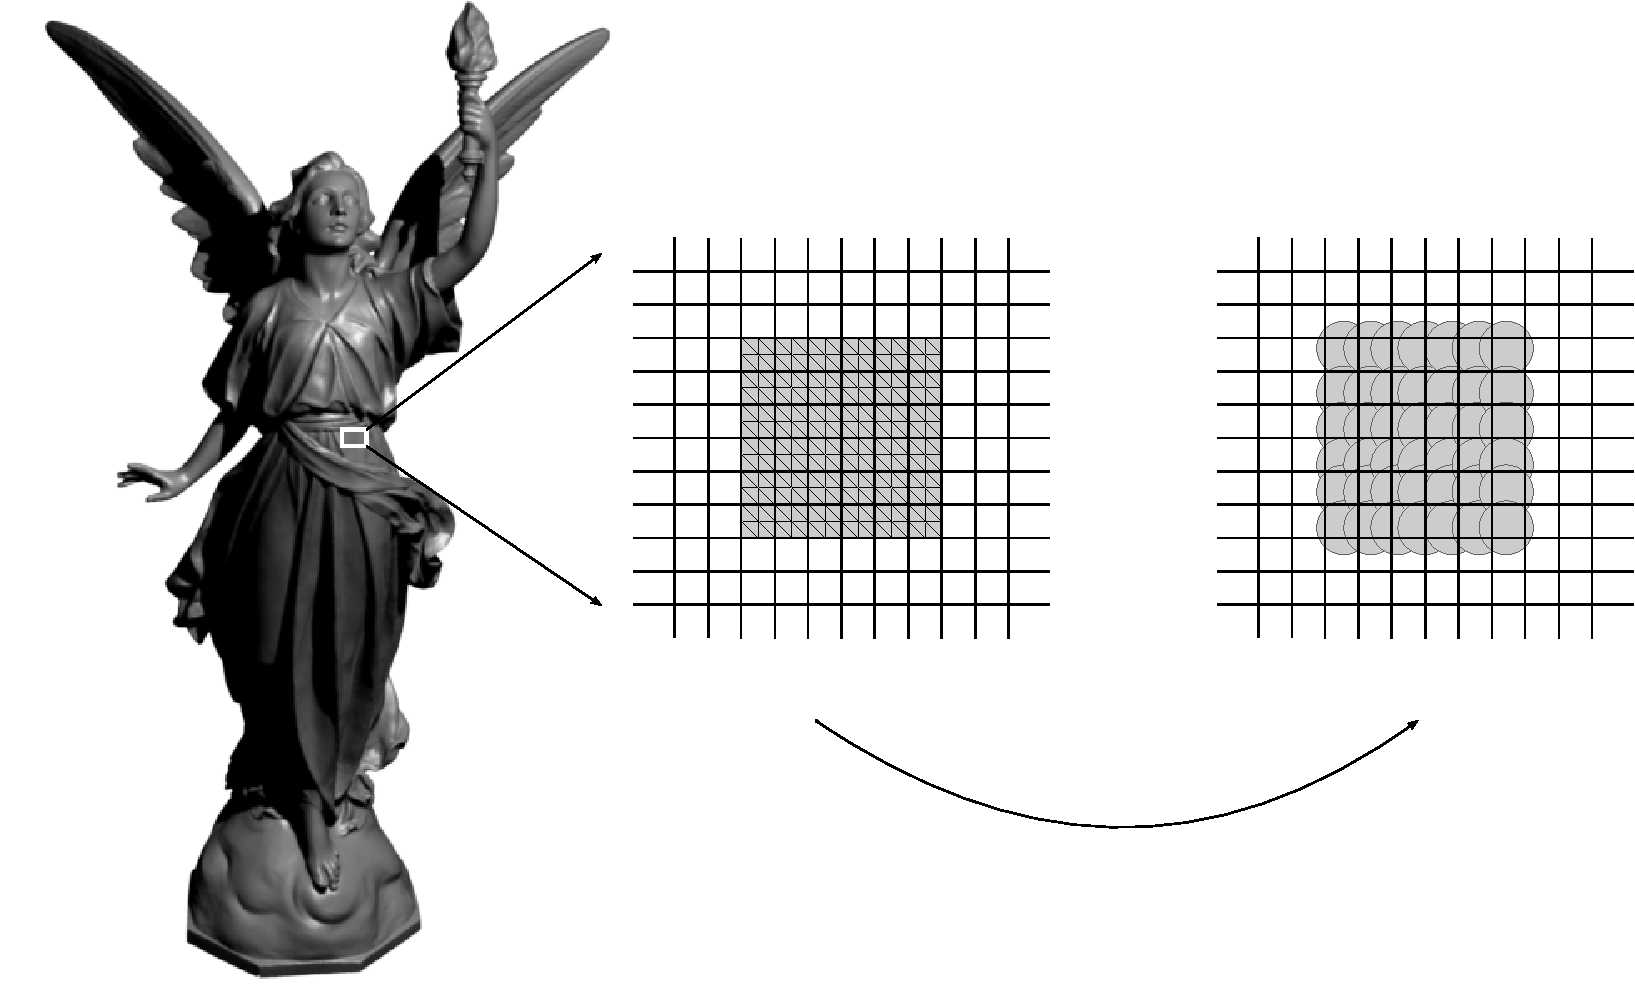
\includegraphics[width=12.0cm]{img/cap01/triangle2point} 
\caption{Lucy figure}
\label{fig:triangle2point}
\end{figure}

H� v�rias raz�es para o sucesso da renderiza��o baseada em pontos. Primeiro,
com o aumento na quantidade de mem�ria das GPUs modernas tornou-se 
poss�vel tratar cenas com quantidade enormes de pol�gonos e como consequ�ncia a
quantidade de pol�gonos que s�o mapeados em menos de um \textit{pixel} �
grande, perdendo-se muito tempo no processo de rasteriza��o(explica��o) como
ilustrado na Figura \ref{fig:triangle2point}. Como as GPUs s�o altamente
otimizadas para renderizar pol�gonos, muitos modelos eram convertidos em um conjunto de pol�gonos usando
m�todos como o algoritmo \textit{marching cubes} \cite{Lorensen1978}. No
entanto as GPUs modernas agora possuem partes de seu \textit{pipeline} gr�fico
program�veis, permitindo a cria��o de algoritmos de renderiza��o alternativos
utilizando-se todo o poder de processamento das GPUs
\cite{Ren2002,Botsch2003,marroquim07}. Segundo, representar superf�cies curvas
usando pol�gonos planares requer informa��o de conectividade e ainda permanecem
como uma aproxima��o da superf�cie curva. Pontos no entanto n�o mant�m esse
tipo de informa��o e opera��es como level de detalhes, deforma��o geom�trica e
modifica��es na topologia s�o f�ceis de implementar.

\section{Objetivo}
\section{Organiza��o da Disserta��o}


  \chapter{Trabalhos Relacionados}

\section{QSplat}
\section{SPT}
\section{Efficiente Point Based Rendering}
\section{Trabalhos relacionados a Simplica��o}
\section{Discussao}




Neste cap�tulo iremos apresentar alguns trabalhos que inspiraram esta
disserta��o, com �nfase em dois deles em particular.
O primeiro � \textit{QSplat} \cite{Rusinkiewicz2000}, um sistema para
renderiza��o de pontos baseado em uma hierarquia de esferas envolventes. O
Segundo � o \textit{Sequential Point Tress} (SPT) \cite{Dachsbacher2003}% 
\abbrev{SPT}{\textit{Sequential Point Trees}}, uma estrutura de dados
que permite-nos renderizar em N�vel de Detalhe e diretamente na GPU
modelos de pontos. E por �ltimo ser�o apresentados outro trabalhos que 
seguem esta mesma linha mas de forma
resumida e com suas principais contribui��es.

\section{\textit{QSplat}}
Nesta se��o iremos descrever o \textit{QSplat}, um sistema para representa��o e
renderiza��o progressiva, de modelos grandes com amostras de $100$ milh�es h�
$1$ bilh�es de pontos como os produzidos no Projeto Michelangelo Digital \cite{Levoy2000}.
\textit{QSplat} combina uma hierarquia de esfera envolventes com renderiza��o
baseado em pontos. Os n�s internos da hierarquia armazenam atributos (posi��o, normal, cor) que s�o
estimados pelos seus n�s filhos. O algoritmo de renderiza��o percorre a
hierarquia at� que o tamanho da proje��o da esfera envolvente seja menor que um
valor pr�-determinado (geralmente um \textit{pixel}). Ent�o o n� � renderizado
e seus filhos podem ser descartados. O sistema ser� descrito com mais detalhes nas se��es seguintes.
\subsection{\textit{QSplat} Estrutura de Dados}
\textit{QSplat} usa uma hierarquia de esfera envolventes que tamb�m � usada
para controle de n�vel de detalhe, \textit{view frustum cullling} e
\textit{back facing culling} \cite{Rusinkiewicz2000}. Cada n� da hierarquia
contem o centro e o raio da esfera envolvente, uma normal, o �ngulo do cone
de normais e uma cor (opcional). A hierarquia � criada em um pr�-processamento
e guardada em disco. Na Figura \ref{fig:schematicQSplat} temos uma esquema de como seria a hierarquia.

\begin{figure}[ht]
\centering
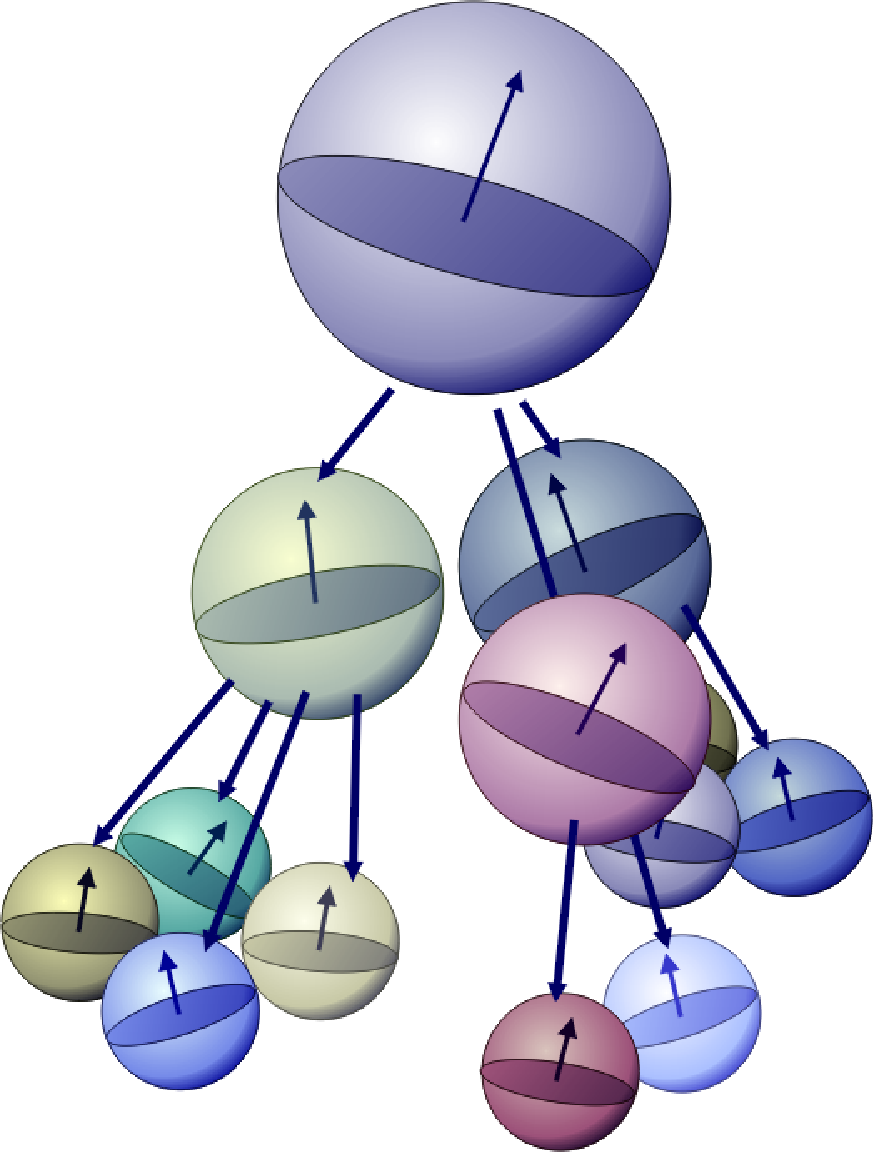
\includegraphics[width=8.0cm]{img/cap02/schematicQSplat} 
\caption{Figura esquem�tica da hierarquia de esferas de
\textit{QSplat} (Retirada de \cite{Wand2004})}
\label{fig:schematicQSplat}
\end{figure}

A estrutura de cada n� na hierarquia de esferas � mostrada na Figura
\ref{fig:NodeQSplat}. Um n� contem a posi��o e o tamanho da esfera  relativa a
seus parentes, normal, cone de normais e uma cor (opcional) e poucos
\textit{bits} que representam a estrutura da �rvore.

\begin{figure}[ht]
\centering
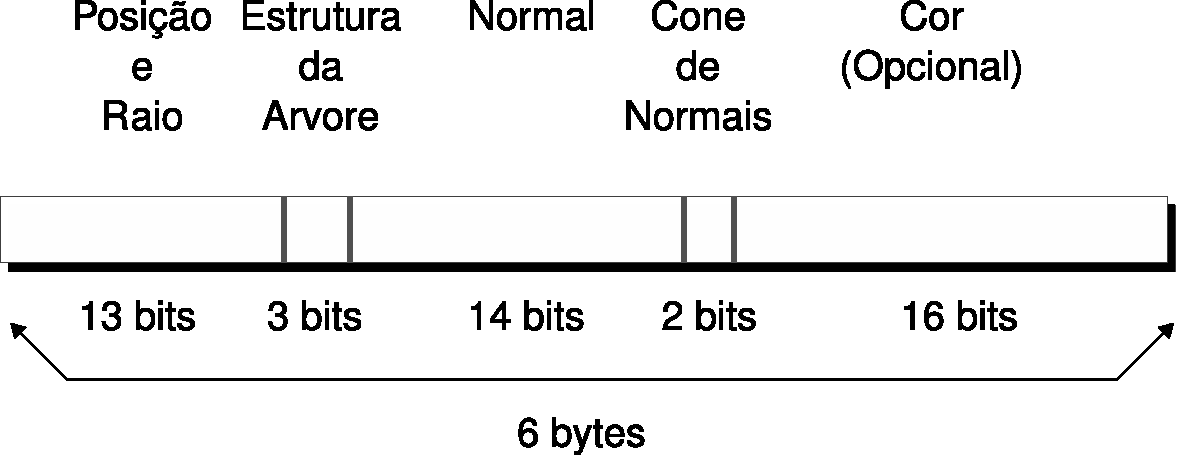
\includegraphics[width=12.0cm]{img/cap02/NodeQuantization} 
\caption{Estrutura de um N�}
\label{fig:NodeQSplat}
\end{figure}

\begin{description}
\item[Posi��o e Raio:]{ A posi��o e o raio de cada esfera � codificada
relativamente aos seus parentes na hierarquia de esferas envolventes. A fim de  
economizar mem�ria, seus valores s�o quantizados em $13$ valores. Ent�o o
raio de um esfera varia de $113$ a $1313$ do raio de seus
parentes e seu centro relativo ao centro de seus parentes (em cada um dos suas
coordenadas $X$, $Y$ e $Z$) � algum m�ltiplo de $113$. Para garantir
que a processo de quantiza��o n�o introduza nenhum buraco durante a
renderiza��o, todos ou valores s�o arredondados para o maior valor que englobe
seus parentes}
\item[Normal]{A normal � codificada em $14$ \textit{bits}. Sua quantiza��o
usa um grade de $52$$x$$52$ em cada uma das $6$ faces do cubo. Um tabela �
usada para decodificar a normal representada. Na pr�tica s�o usados
$52\cdot52\cdot6 = 16224$  diferentes valores de normal}
\item[Color]{O anglo do cone de normais � codificado em apenas $2$
\textit{bits}. Os quatros valores poss�veis que representam o metade do
anglo de abertura do cone s�o $116$, $416$, $916$ e
$1616$ }
\item[Cor]{D�vida \ldots}
\end{description}
\subsection{Renderiza��o}
O processo de renderiza��o � simples, como mostrado na Figura
\ref{fig:percorrimento}. Os est�gios do algoritmo ser�o mostrados a seguir.

\begin{description}
\item[\textit{Visible Culling}]{Como � usado um hierarquia de esferas
envolventes, n�s que n�o s�o vis�veis s�o eliminados durante o percurso.
\textit{Frustum Culling} � feito, testando cada esfera contra os planos do
tronco de pir�mide que representa o campo de vis�o. Se a esfera est� fora, ela
e sua sub-�rvore s�o eliminados. Se ela est� dentro do
campo de vis�o, ela e seus filhos est�o vis�veis e n�o precisam mais passar
pelo teste. \textit{Backface Culling} tamb�m � realizados durante o processo de
renderiza��o, usando o �ngulo do cone de normais.}
\item[Heur�stica de Renderiza��o]{A heur�stica usando � o tamanho da imagem
projetada na tela, ou seja, �rea da esfera projetada na tela exceder
um determinado valor (geralmente um \textit{pixel}).}
\item[Renderizando um \textit{Splat}] Quando se atinge um n� desejado, de
acordo com os crit�rios mencionados anteriormente, o \textit{splat} �
renderizado representando a esfera corrente. O tamanho do \textit{splat} �
baseado no di�metro da proje��o da esfera corrente, e sua cor � obtida usando
c�lculo de ilumina��o baseada na normal e cor da mesma.

\end{description}

\begin{figure}[tcb]
  \centering \mbox{} \hfill
  \begin{minipage}[b]{0.45\linewidth}
 \centering
  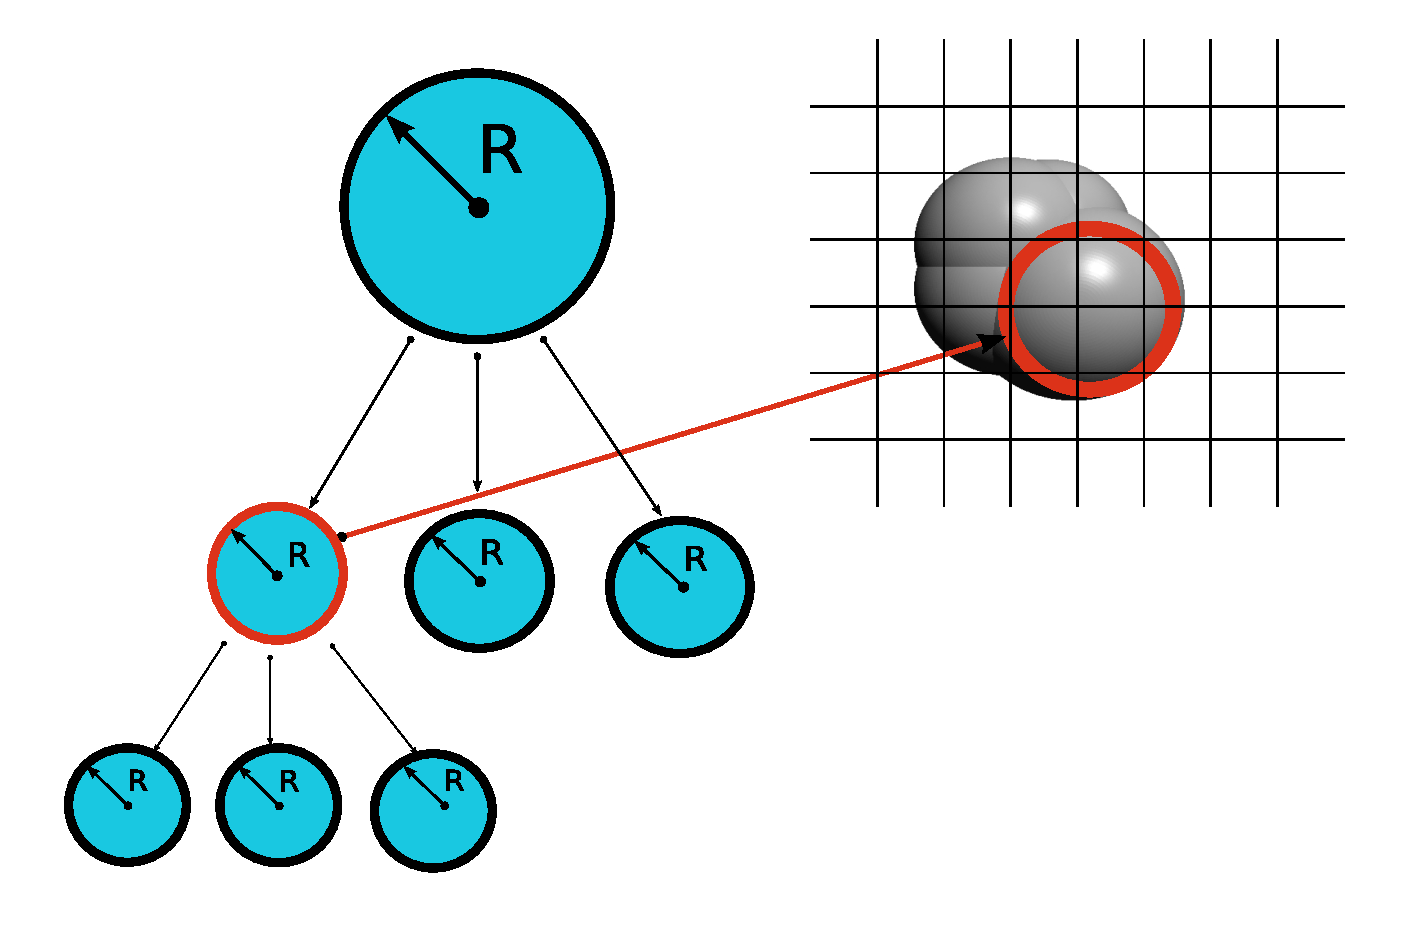
\includegraphics[width=1.25\linewidth]{img/cap02/ovoRender}\\[0cm](a)
  \end{minipage}
  \hfill
  \begin{minipage}[b]{0.45\linewidth}
    \centering
    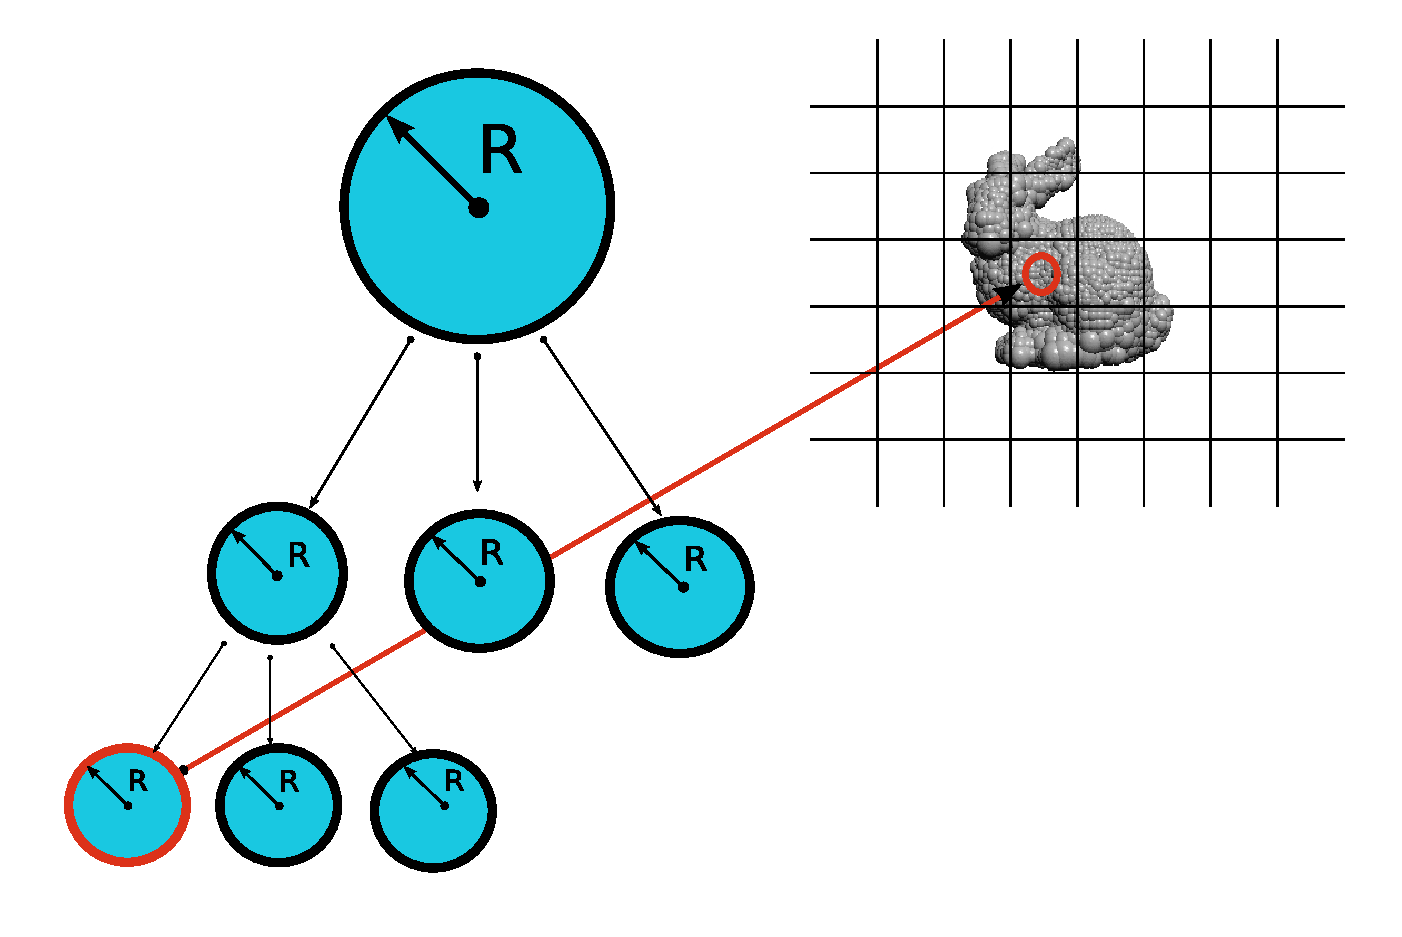
\includegraphics[width=1.25\linewidth]{img/cap02/CoelhoRender}\\[0cm](b)
  \end{minipage}
  \hfill \mbox{}
  \caption{\label{fig:percorrimento}Esquema do algoritmo de renderiza��o:  
  \emph{(a)} Tamanho da imagem projetada do n� � maior que um \textit{pixel}.
  Continua o percurso nas sub-�rvores; \emph{(b)} Tamanho da imagem
  projetada do n� � menor que um \textit{pixel}. Renderiza o \textit{splat}.}
\end{figure}

\subsection{Discuss�o}
\textit{QSplat} possui um processo bem simples, mas infelizmente ele n�o usa
todo o potencial gr�fico que as GPUs oferecem. Dada
granularidade na sua determina��o de n�vel de detalhes, um modelo chega e ser
renderizado ponto por ponto. Como consequ�ncia, esse ``modo imediato'' de
renderizar torna a GPU pouco utilizada, pois est� sempre esperando
por novos dados para renderizar. Levando em conta que n�o � apenas a coordenada
de um ponto que est� sendo utilizada, mas todos os seus outros atributos, como
cor e normal.

No entanto, est� simplicidade torna o \textit{Qsplat} um algoritmo que pode ser
usado em outras aplica��es. Sua hierarquia de esfera � uma boa estrutura para
\textit{Ray Tracing}. Outra s�o aplica��es em rede como a do \textit{Stream
QSplat}\cite{Rusinkiewicz2001} que permite visualizar modelos $3D$ de forma
progressiva e remotamente.


\section{\textit{Sequential Point Trees}}
\textit{QSplat} possui um processamento de dados muito simples e de f�cil
implementa��o, mas infelizmente sua estrutura hier�rquica recursiva � dif�cil de
ser implementada em GPU. Os pontos renderizados n�o s�o armazenados de forma
cont�nua, portanto n�o s�o processados sequencialmente.A \textit{CPU}
(\textit{Central Processor Unit})%
\abbrev{CPU}{\textit{Central Processor Unit}} percorre a
�rvore e faz chamadas independentes para renderizar cada n�. Isso causa um
``gargalo'' entra a CPU e a GPU, sendo que esta �ltima fica muito tempo ociosa
esperando por dados da CPU.
\textit{Sequential Point Trees} prop�e o uso da estrutura de \textit{QSplat},
s� que de uma forma sequencial que � facilmente tratada em GPU. Sendo assim,
transferindo mais trabalho para GPU e diminuindo este ``gargalo''.
Nas se��es que seguem , SPT ser� apresentado com mais detalhes. 
\subsection{Hierarquia de Pontos}
Inicialmente SPT possui um hierarquia de pontos representada por um
\textit{Octree} \cite{Samet05}. Cada n� da hierarquia representa parte do
objeto. Ela armazena um centro \textbf{c} e uma estimativa da normal
\textbf{n}. Um n� armazena tamb�m um di�metro \textbf{d} da esfera envolvente
centrada em \textbf{c}. O n� interior representa
a uni�o de seus n�s filhos, ent�o o di�metro cresce a medida que sobe na
hierarquia. Os n�s folhas possuem pontos que s�o distribu�dos uniformemente no
objeto, ent�o possuem di�metro aproximadamente iguais.

\subsection{M�tricas de Erro}

Cada n� na hierarquia pode ser aproximada por um disco com o mesmo centro,
normal e di�metro do n�. O erro dessa aproxima��o � descrito por dois valores
: o erro perpendicular $e_p$ e o erro tangencial $e_t$.
 
\noindent \textbf{Erro Perpendicular:}
O erro perpendicular $e_p$ � a dist�ncia m�nima entre dois planos
paralelo ao disco que engloba todos os filhos. Este erro mede vari�ncia e pode ser
calculado como:

\begin{figure}[tcb]
  \centering \mbox{} \hfill
  \begin{minipage}[b]{0.40\linewidth}
 \centering
 
  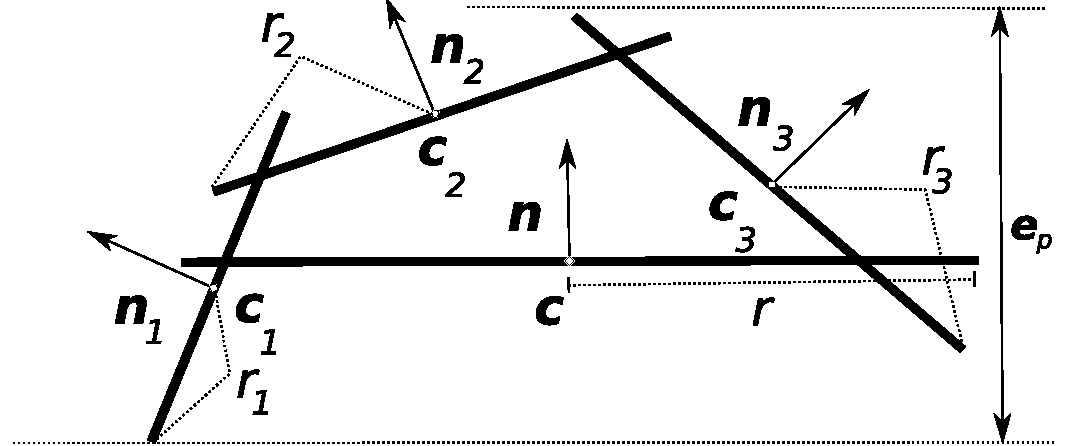
\includegraphics[width=1.0\linewidth]{img/cap02/PosterSquential}
  \end{minipage}
  \hfill
  \begin{minipage}[b]{0.40\linewidth}
    \centering
    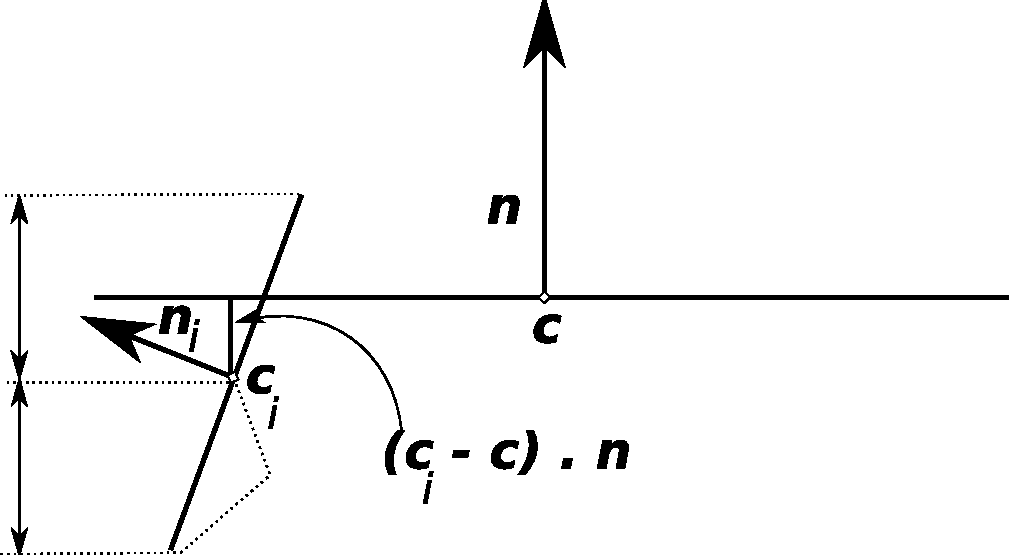
\includegraphics[width=1.0\linewidth]{img/cap02/di}
  \end{minipage}
  \hfill \mbox{}
  \caption{\label{fig:perpendicular}Como erro perpendicular, usa-se a
  dist�ncia entre dois plano paralelo ao disco que engloba todos os filhos
  (Retirada de \cite{Dachsbacher2003}).}
\end{figure}

\begin{eqnarray}
 e_p & = & max\{((c_i-c)\cdot n)+d_i\} - min\{((c_i-c)\cdot n )-d_i\} \\
     &   &\textnormal{with}\hspace{0.5cm}  d_i = r_i \sqrt{1-(n_i\cdot n)^2}
  \label{perpendicular}
\end{eqnarray}

Durante a renderiza��o, o erro perpendicular � projetado na imagem, resultando
em um erro $\tilde{e}_p$. $\tilde{e}_p$ � proporcional ao seno do �ngulo entre
o vetor de vis�o $v$ e a normal do disco $n$ e diminui com $\cfrac{1}{r}$ e $r =
|v|\cdot\tilde{e}_p$ captura erros ao longo das silhuetas:
 
 \begin{equation}
  \tilde{e}_p  = e_p \frac{\sin{(\alpha)}}{r} \quad \text{sendo} \quad \alpha =
  \angle(n,v)
   \label{tangencial}
 \end{equation}

\noindent \textbf{Erro Tangencial:}
O erro tangencial $e_t$, analisa a proje��o dos discos dos filhos no
disco do pai como mostrado na Figura \ref{fig:Tangencial}. $e_t$ mede se o
disco pai cobre um grande �rea desnecess�ria. O erro � medido usando v�rias
retas ao redor dos filhos projetados. $e_t$ � portanto o menor di�metro do
disco pai menos o tamanho do menor intervalo entre retas. (d�vida em rela��o a
escrita). $e_t$ negativos s�o setados em zero. $e_t$ � projetado no espa�o de
imagem como:

\begin{equation}
 \tilde{e}_t = e_t \frac{\cos{(\alpha)}}{r} 
  \label{tangencial}
\end{equation}

\noindent \textbf{Erro Geom�trico:}
O erro perpendicular e tangencial podem ser combinados em um �nico erro
geom�trico:
Agora o erro no espa�o de imagem $\tilde{e}_g$ depende apenas de $r$, e n�o mais
do �ngulo do vis�o: $ \tilde{e}_g = \cfrac{e_g}{r}$
 
 \begin{equation}
 \tilde{e}_g  = \max\{e_p\sin{\alpha} + e_t\cos{\alpha}\} = \sqrt{e^2_p + e^2_t} 
  \label{tangencial}
\end{equation}

\begin{figure}[ht]
\centering
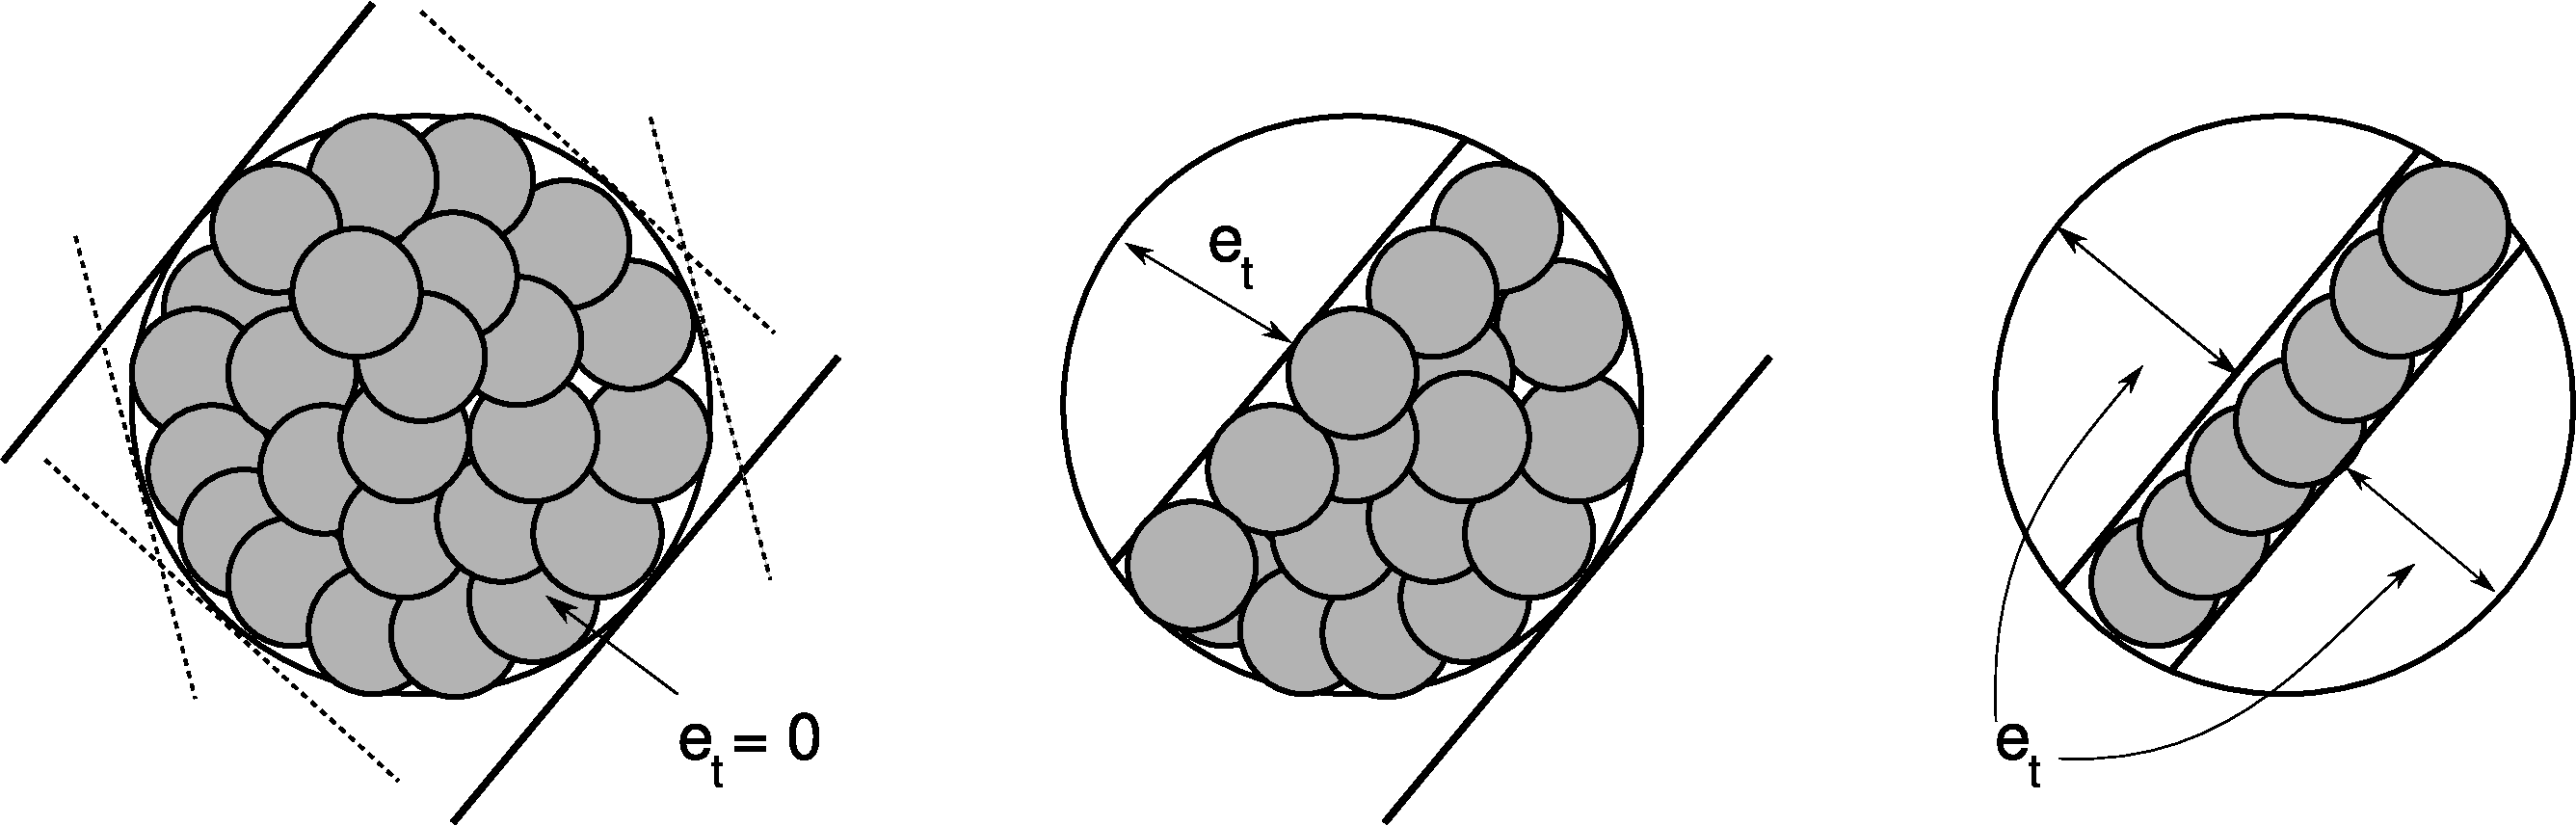
\includegraphics[width=15.0cm]{img/cap02/tangencial} 
\caption{Erro tangencial, mede o qu�o aproximado � o disco pai em rela��o ao
filho no plano tangente (Retirada de \cite{Dachsbacher2003}) .}
\label{fig:Tangencial}
\end{figure}

\subsection{Renderiza��o Recursiva}
Um objeto � renderizado na hierarquia de pontos usando um percurso em
profundidade. Para cada n� um erro de imagem $\tilde{e}_g$ � calculado. Se
$\tilde{e}_g$ est� abaixo de um limite de erro estabelecido $\epsilon$ e o n�
n�o � uma n� folha , seus filhos s�o percorridos recursivamente. Por outro lado,
um \textit{splat} de tamanho $\tilde{d} =  d/r$ � renderizado. Note que
esta hierarquia de pontos n�o se adapta apenas a dist�ncia do observador $r$,
mas tamb�m para propriedades da superf�cie. Grandes �reas planas s�o detecta-das
com pequenos erro geom�trico $\tilde{e}_g$ e podem ser renderizados com splats
grandes.
\subsection{Rearranjamento}
O procedimento de renderiza��o da se��o anterior � recursivo e n�o se adapta ao
processamento to r�pido e sequ�ncial da GPU. Assim, h� um rearranjamento da
estrutura em �rvore para um estrutura em lista e o teste recursivo �
substitu�do por um percorrimento sequ�ncial sobre a lista de pontos.

Para isso, o erro simplificado $\tilde{e}_g$ � substitu�do por um que sejam
mais intuitivo. Assume-se que $\epsilon$ � constante. O teste
recursivo � $\tilde{e}_g = {e}_g/r < \epsilon $ e ao inv�s de $e_g$, �
armazenado um dist�ncia m�nima $r_{\min} = e_g/ \epsilon$ que simplifica o
teste recursivo para $r > r_{\min}$. Entretanto, quando os n�s da �rvore s�o
processados seq�encialmente sem informa��o hier�rquica, h� necessidade de um
teste n�o recursivo. Para esse fim, � adicionado um par�metro $r_{\max}$, que �
simplesmente um $r_{\min}$ do seu n� pai, em cada n� e usa-se $r \in
[r_{\min},r_{\max}]$ como um teste n�o recursivo. Desta maneira pode-se guiar o
algoritmo de renderiza��o com esse teste \textit{intercalar} para cada n�.

\begin{figure}[tcb]
  \centering \mbox{} \hfill
  \begin{minipage}[b]{0.40\linewidth}
 \centering
  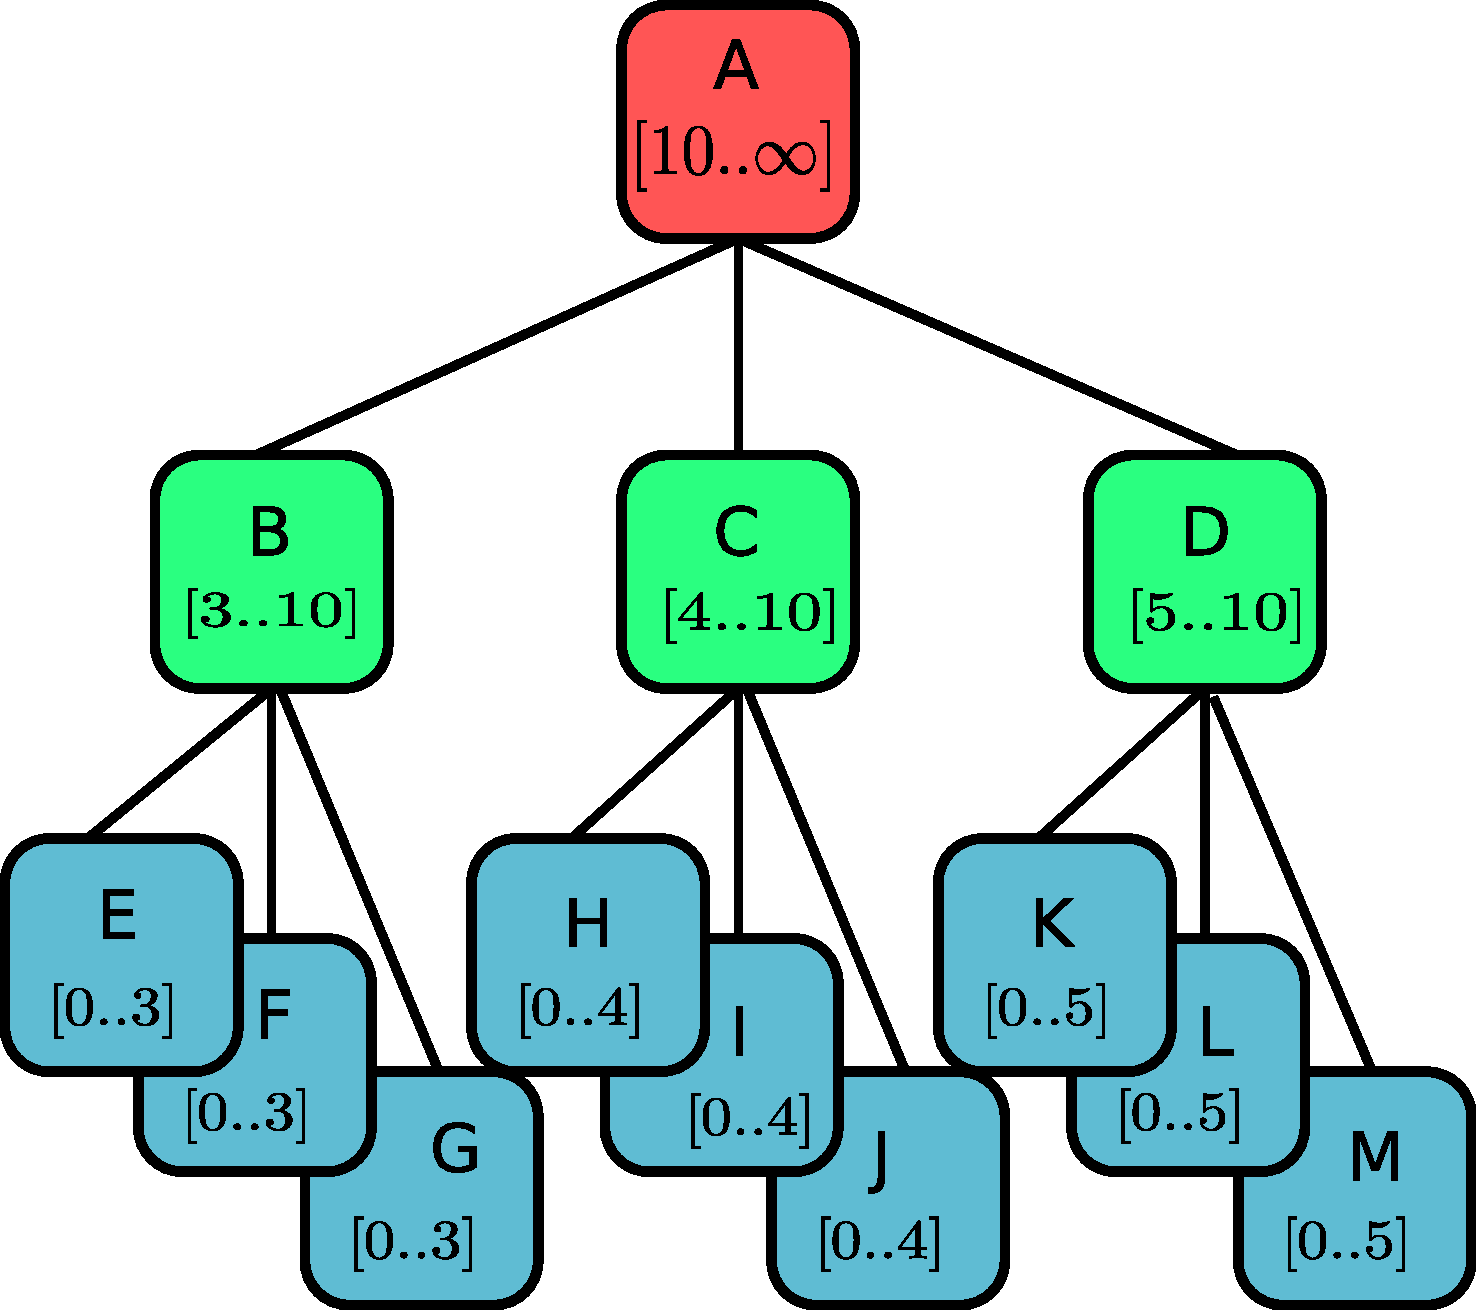
\includegraphics[width=1.0\linewidth]{img/cap02/SequentialTree}\\[0cm](a)
  \end{minipage}
  \hfill
  \begin{minipage}[b]{0.40\linewidth}
    \centering
    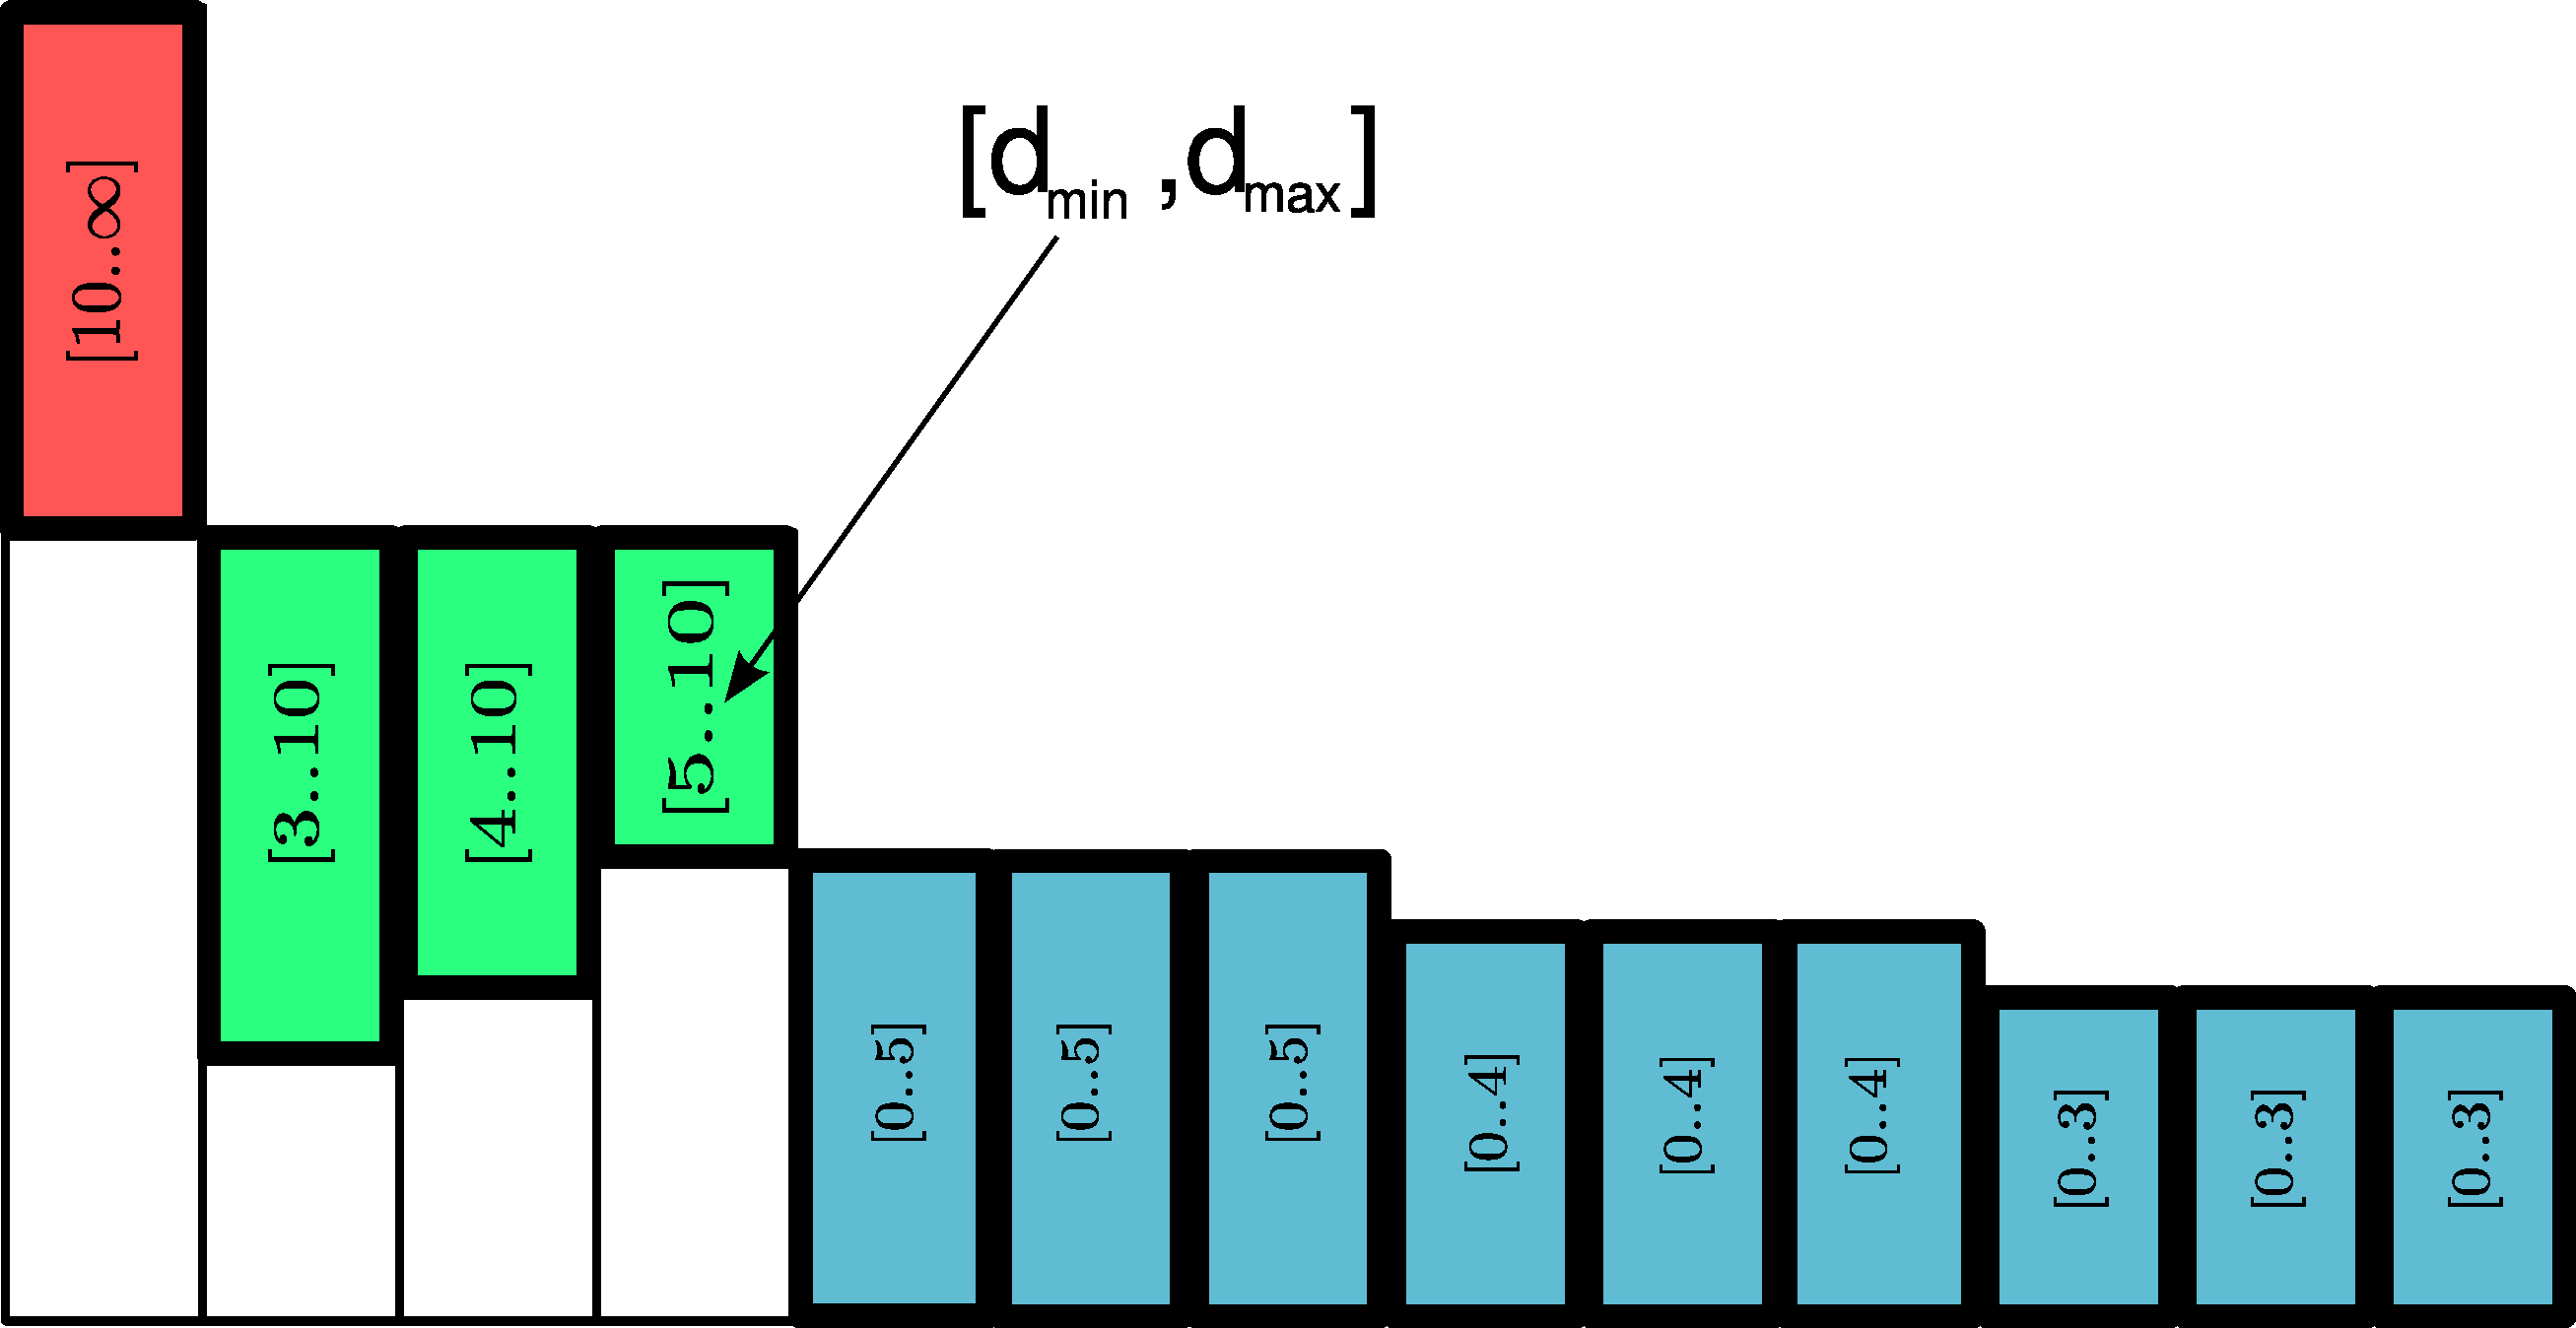
\includegraphics[width=1.2\linewidth]{img/cap02/SequentialDamx}\\[0cm](b)
  \end{minipage}
  \hfill \mbox{}
  \caption{\label{fig:list}Como erro perpendicular, usa-se a
  dist�ncia entre dois planos paralelos ao disco que engloba todos os filhos
  (adaptada de \cite{Dachsbacher2003}).}
\end{figure}


Depois de substituir o teste recursivo por um simples teste intervalar, a
hierarquia de pontos e transformada em um lista, que � processada
sequencialmente. Neste est�gio, $[r_{\min},r_{\max}]$ � usada para ordenar a
lista de forma decrescente a partir de $r_{\max}]$ como ilustrado na
Figura \ref{fig:list}.

Um exemplo de como o algoritmo de renderiza��o funciona � mostrado na Figura
\cite{fig:SequentialList}. Onde para diferentes valores de $r$ um por��o da
lista � selecionada enquanto outras s�o descartadas.

\begin{figure}[ht]
\centering
\includegraphics[width=15.0cm]{img/cap02/SequentialList} 
\caption{Erro tangencial, mede o qu�o aproximado � o disco pai em rela��o ao
filho no plano tangente (Retirada de \cite{Dachsbacher2003}) .}
\label{fig:SequentialList}
\end{figure}

\subsection{Discuss�o}

SPT � simples, de f�cil implementa��o e prov� um renderiza��o continua usando
n�vel de detalhes.

O autor da �nfase no fato de que grande parte do trabalho � movido para GPU,
deixando a CPU livre para outras tarefas. No entanto, SPT s� � eficiente se o modelo 
estiver na mem�ria de v�deo, o que nem sempre � poss�vel.

SPT renderiza pontos em baixa qualidade, j� que a GPU n�o suporta renderizar
\textit{splat} com qualidade em tempo satisfat�rio. Outra desvantagem � que SPT
n�o realiza \textit{frustum culling}, perdendo o pouco em efici�ncia.

  \chapter{Estruturas de Dados para Pontos}
\label{chapter:3}
\section{Estrutura de Parti��o do Espa�o}
O objetivo de um estrutura de parti��o do espa�o � criar uma indexa��o do
espa�o, ou seja, decompo-l� em c�lulas e prov� uma rela��o entre estas c�lulas
e o espa�o ocupado por um objeto \cite{S}.
\subsection{Estruturas Hieraquicas}
Esquemas de parti��o do espa�o s�o comuns(?) em computa��o gr�fica, em
particular quando se deseja processar geometria adquirida � ess�ncial:
simplifica��o, reconstru��o, compress�o, visibilidade, e muita outras
opera��es s�o beseadas em nesse tipo de estrutura. Sua simplicidade a tornou
muito popular: o espa�o inicial, frequentimente uma caixa envolvente do modelo,
� recursivamente subdividida at� que uma celula satisfa�a um dado crit�rio. As
estutras de parti��o de espa�o mais populares s�o, \textit{octree} e 
\textit{kD-Trees} (um caso especial de  \textit{BSP-Tree}). Primeiramente,
\textit{octree} ser� discutida na sess�o \ref{section:Octree}, que � obtida
particionando recursivamente a caixa envolvente do modelo em oito octantes.
Na proxima sess�o \ref{section:KDtree} apresentaremos \textit{K-d Tree} que
tamb�m particona o espa�o, mas dividindo o modelo em cada n� de acordo com uma
dimens�o. \textit{K-d Tree} ser� usada como estrutura eficente de busca dos $k$
vizinhos de um dado ponto no modelo. Finalmente, hieraruia de
esferas envolventes ser� discutida (\ref{section:BVH}).

\subsubsection{Octrees}
\label{section:Octree}
\textit{Octree} � uma das estruturas de parti��o espacial mais usadas para
tratar grandes modelos de pontos em especial, quando se quer renderiz�-los de forma interativa [cites].
 A estrutura � usada para particionar a caixa envolvente $3D$ que
engloba todas as amostras no espa�o. Cada c�lula  que contenha amostras �
recursivamente subdivida em oito octantes.A recurs�o termina quando em uma
c�lula h� um valor m�nimo de amostras que passa a ser um cont�iner de amostras
desta c�lula (seriam as folhas de uma estrutura em �rvore).

Octree sobre um conjuntos $P$ de  $n$ pontos $p_{1 \ldots n}$ � constru�da de
forma eficiente com complexidade de $O(n\log{n})$

\subsubsection{kd-Tree}
\label{section:KDtree}
Uma \textit{kd-tree} � em geral , um �rvore multidimensional de busca em $k$
dimens�es. Para dados em $3D$, a �rvore correspondente � geralmente chamada de \textit{kd-tree}
tridimensional ao inv�s de \textit{$3d$-tree}. Elas s�o um caso especial de
arvores parti��o bin�ria espacial \abbrev{PBE}{\textit{parti��o
bin�ria espacial}} . \textit{Kd-tree} usa planos de cortes que s�o perpendicular
a um dos eixos coordenados ( tamb�m chamado hiperplanos), que � uma
especializa��o de uma $PBE$, em que planos de cortes arbitr�rios podem ser
usados. Um conjunto de pontos em uma \textit{kd-tree} � subdividido em caixas
alinhas aos eixos e que n�o se interceptam. O algoritmo de constru��o �
descrito como o exemplificado:

Na raiz, o conjunto de pontos � dividido em dos subconjuntos com o mesmo
tamanho por um hiperplano perpendicular ao eixo dos $x$. Os filhos da raiz
(profundidade $1$), a parti��o � baseada na coordenada $y$ e o n� de
profundidade $2$, no pr�ximo level, na coordenada $z$. Ent�o o algoritmo come�a
ordenando o conjunto de pontos na coordenada $x$. A recurs�o para quando um
determinada quantidade de pontos em um n� � alcan�ada (no caso um ponto, veja
\ref{fig:Kdtree}), o qual � armazenados nas folhas.

\begin{figure}[ht]
\centering
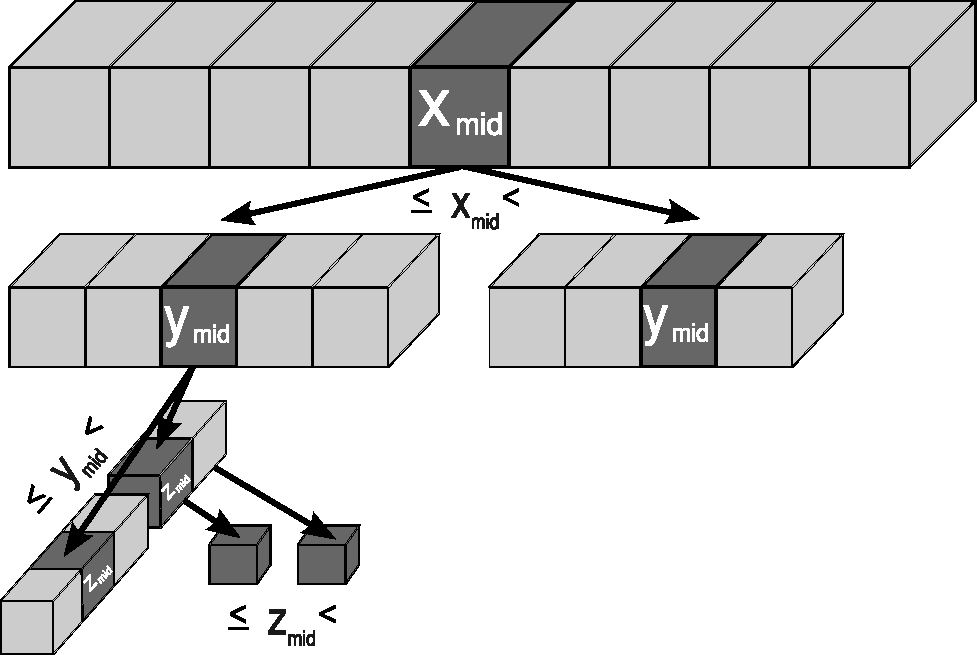
\includegraphics[width=10.0cm]{img/cap02/Kd-tree} 
\caption{Kd-Tree}
\label{fig:Kdtree}
\end{figure}

\subsubsection{Hierarquia de Volumes Envolventes}
\label{section:BVH}
Hierarquia de Volumes Envolventes (BVH) tem sido usado para renderiza��o desde
Clark and Rubin and Whitted [cite], uso-as como suporte para consultas como \textit{visibilty culling} 
e intersec��o de raio-objeto. Enquanto m�todo de parti��o de dados para
indexa��o no espa�o, como \textit{Octrees} e \textit{Kd-Trees} descritas
anteriormente, BVH n�o precisam ser uma parti��o do espa�o. Sendo assim, BVH
remove qualquer restri��o em rela��o a parti��o do espa�o e permite a
constru��o de uma hierarquia espacial mais gen�rica. De fato, ela permite
qualquer hierarquia que agrupe os elementos, sem entretanto prov� uma sele��o
espacial que � de fundamental import�ncia para qualquer esquema de indexa��o
espacial. O �nico requisito em uma BVH � que cada n� o volume envolvente (i.e.,
uma caixa ou esfera) engloba todos os elementos da sua sub�rvore. Obviamente
que uma estrutura de parti��o espacial pode ser estendida para uma BVH, gerando
o volume envolvente atribu�do a cada n� como mostrado anteriormente.

\section{Multiresolu��o e N�vel de Detalhe}
Neste sess�o iremos apresentar alguns trabalhos que inspiraram esta
disserta��o, com �nfase em dois deles em particular.
O primeiro � \textit{QSplat} \cite{Rusinkiewicz2000}, um sistema para
renderiza��o de pontos baseado em uma hierarquia de esferas envolventes. O
Segundo � o \textit{Sequential Point Tress} (SPT) \cite{Dachsbacher2003}% 
\abbrev{SPT}{\textit{Sequential Point Trees}}, uma estrutura de dados
que permite-nos renderizar em N�vel de Detalhe e diretamente na GPU
modelos de pontos. E por �ltimo ser�o apresentados outro trabalhos que 
seguem esta mesma linha mas de forma
resumida e com suas principais contribui��es.
\section{\textit{QSplat}}
Nesta se��o iremos descrever o \textit{QSplat}, um sistema para representa��o e
renderiza��o progressiva, de modelos grandes com amostras de $100$ milh�es h�
$1$ bilh�es de pontos como os produzidos no Projeto Michelangelo Digital \cite{Levoy2000}.
\textit{QSplat} combina uma hierarquia de esfera envolventes com renderiza��o
baseado em pontos. Os n�s internos da hierarquia armazenam atributos (posi��o, normal, cor) que s�o
estimados pelos seus n�s filhos. O algoritmo de renderiza��o percorre a
hierarquia at� que o tamanho da proje��o da esfera envolvente seja menor que um
valor pr�-determinado (geralmente um \textit{pixel}). Ent�o o n� � renderizado
e seus filhos podem ser descartados. O sistema ser� descrito com mais detalhes nas se��es seguintes.
\subsection{\textit{QSplat} Estrutura de Dados}
\textit{QSplat} usa uma hierarquia de esfera envolventes que tamb�m � usada
para controle de n�vel de detalhe, \textit{view frustum cullling} e
\textit{back facing culling} \cite{Rusinkiewicz2000}. Cada n� da hierarquia
contem o centro e o raio da esfera envolvente, uma normal, o �ngulo do cone
de normais e uma cor (opcional). A hierarquia � criada em um pr�-processamento
e guardada em disco. Na Figura \ref{fig:schematicQSplat} temos uma esquema de como seria a hierarquia.

\begin{figure}[ht]
\centering
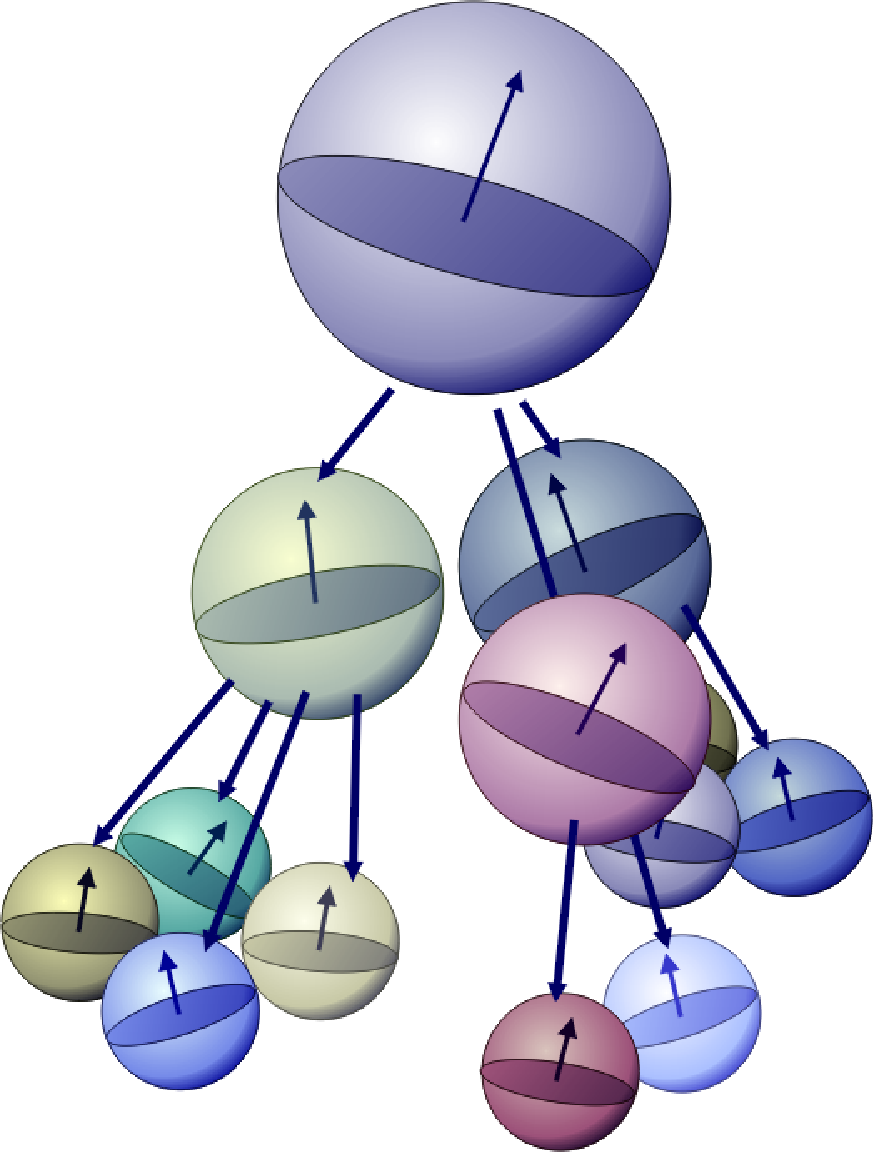
\includegraphics[width=8.0cm]{img/cap02/schematicQSplat} 
\caption{Figura esquem�tica da hierarquia de esferas de
\textit{QSplat} (Retirada de \cite{Wand2004})}
\label{fig:schematicQSplat}
\end{figure}

A estrutura de cada n� na hierarquia de esferas � mostrada na Figura
\ref{fig:NodeQSplat}. Um n� contem a posi��o e o tamanho da esfera  relativa a
seus parentes, normal, cone de normais e uma cor (opcional) e poucos
\textit{bits} que representam a estrutura da �rvore.

\begin{figure}[ht]
\centering
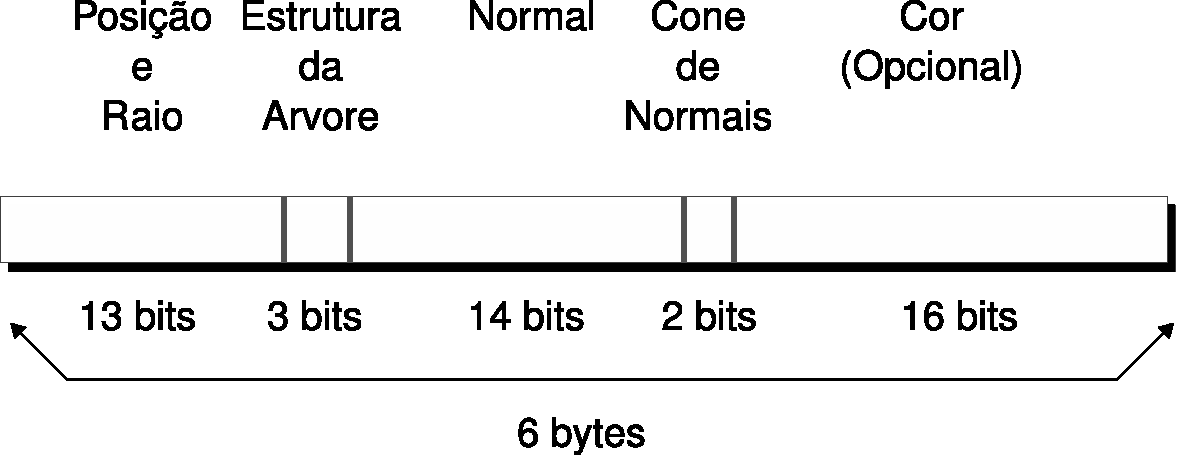
\includegraphics[width=12.0cm]{img/cap02/NodeQuantization} 
\caption{Estrutura de um N�}
\label{fig:NodeQSplat}
\end{figure}

\begin{description}
\item[Posi��o e Raio:]{ A posi��o e o raio de cada esfera � codificada
relativamente aos seus parentes na hierarquia de esferas envolventes. A fim de  
economizar mem�ria, seus valores s�o quantizados em $13$ valores. Ent�o o
raio de um esfera varia de $113$ a $1313$ do raio de seus
parentes e seu centro relativo ao centro de seus parentes (em cada um dos suas
coordenadas $X$, $Y$ e $Z$) � algum m�ltiplo de $113$. Para garantir
que a processo de quantiza��o n�o introduza nenhum buraco durante a
renderiza��o, todos ou valores s�o arredondados para o maior valor que englobe
seus parentes}
\item[Normal]{A normal � codificada em $14$ \textit{bits}. Sua quantiza��o
usa um grade de $52$$x$$52$ em cada uma das $6$ faces do cubo. Um tabela �
usada para decodificar a normal representada. Na pr�tica s�o usados
$52\cdot52\cdot6 = 16224$  diferentes valores de normal}
\item[Color]{O anglo do cone de normais � codificado em apenas $2$
\textit{bits}. Os quatros valores poss�veis que representam o metade do
anglo de abertura do cone s�o $116$, $416$, $916$ e
$1616$ }
\item[Cor]{D�vida \ldots}
\end{description}
\subsection{Renderiza��o}
O processo de renderiza��o � simples, como mostrado na Figura
\ref{fig:percorrimento}. Os est�gios do algoritmo ser�o mostrados a seguir.

\begin{description}
\item[\textit{Visible Culling}]{Como � usado um hierarquia de esferas
envolventes, n�s que n�o s�o vis�veis s�o eliminados durante o percurso.
\textit{Frustum Culling} � feito, testando cada esfera contra os planos do
tronco de pir�mide que representa o campo de vis�o. Se a esfera est� fora, ela
e sua sub-�rvore s�o eliminados. Se ela est� dentro do
campo de vis�o, ela e seus filhos est�o vis�veis e n�o precisam mais passar
pelo teste. \textit{Backface Culling} tamb�m � realizados durante o processo de
renderiza��o, usando o �ngulo do cone de normais.}
\item[Heur�stica de Renderiza��o]{A heur�stica usando � o tamanho da imagem
projetada na tela, ou seja, �rea da esfera projetada na tela exceder
um determinado valor (geralmente um \textit{pixel}).}
\item[Renderizando um \textit{Splat}] Quando se atinge um n� desejado, de
acordo com os crit�rios mencionados anteriormente, o \textit{splat} �
renderizado representando a esfera corrente. O tamanho do \textit{splat} �
baseado no di�metro da proje��o da esfera corrente, e sua cor � obtida usando
c�lculo de ilumina��o baseada na normal e cor da mesma.

\end{description}

\begin{figure}[tcb]
  \centering \mbox{} \hfill
  \begin{minipage}[b]{0.45\linewidth}
 \centering
  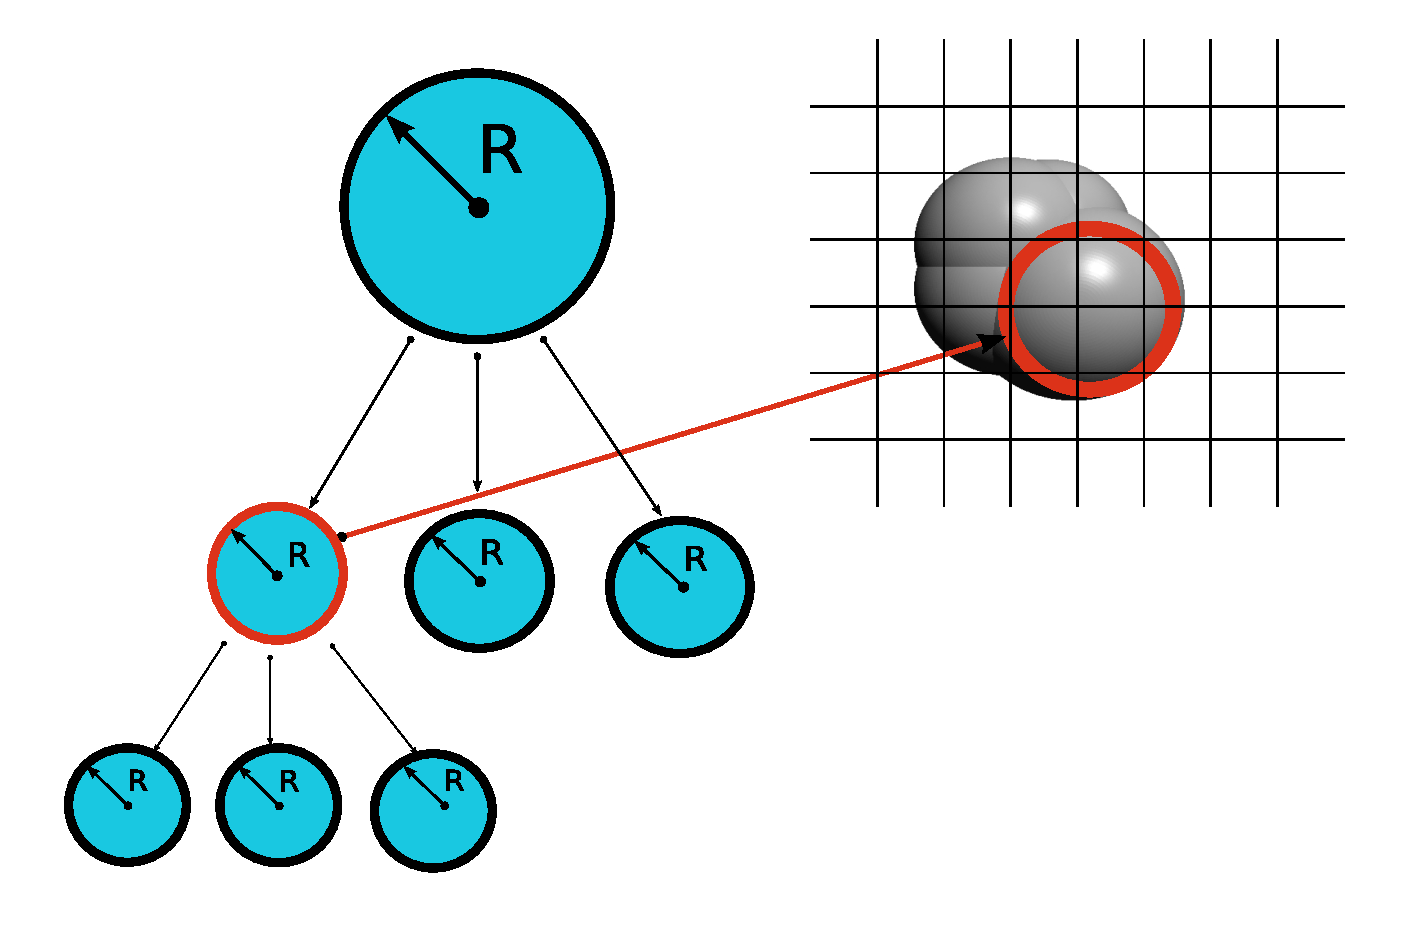
\includegraphics[width=1.25\linewidth]{img/cap02/ovoRender}\\[0cm](a)
  \end{minipage}
  \hfill
  \begin{minipage}[b]{0.45\linewidth}
    \centering
    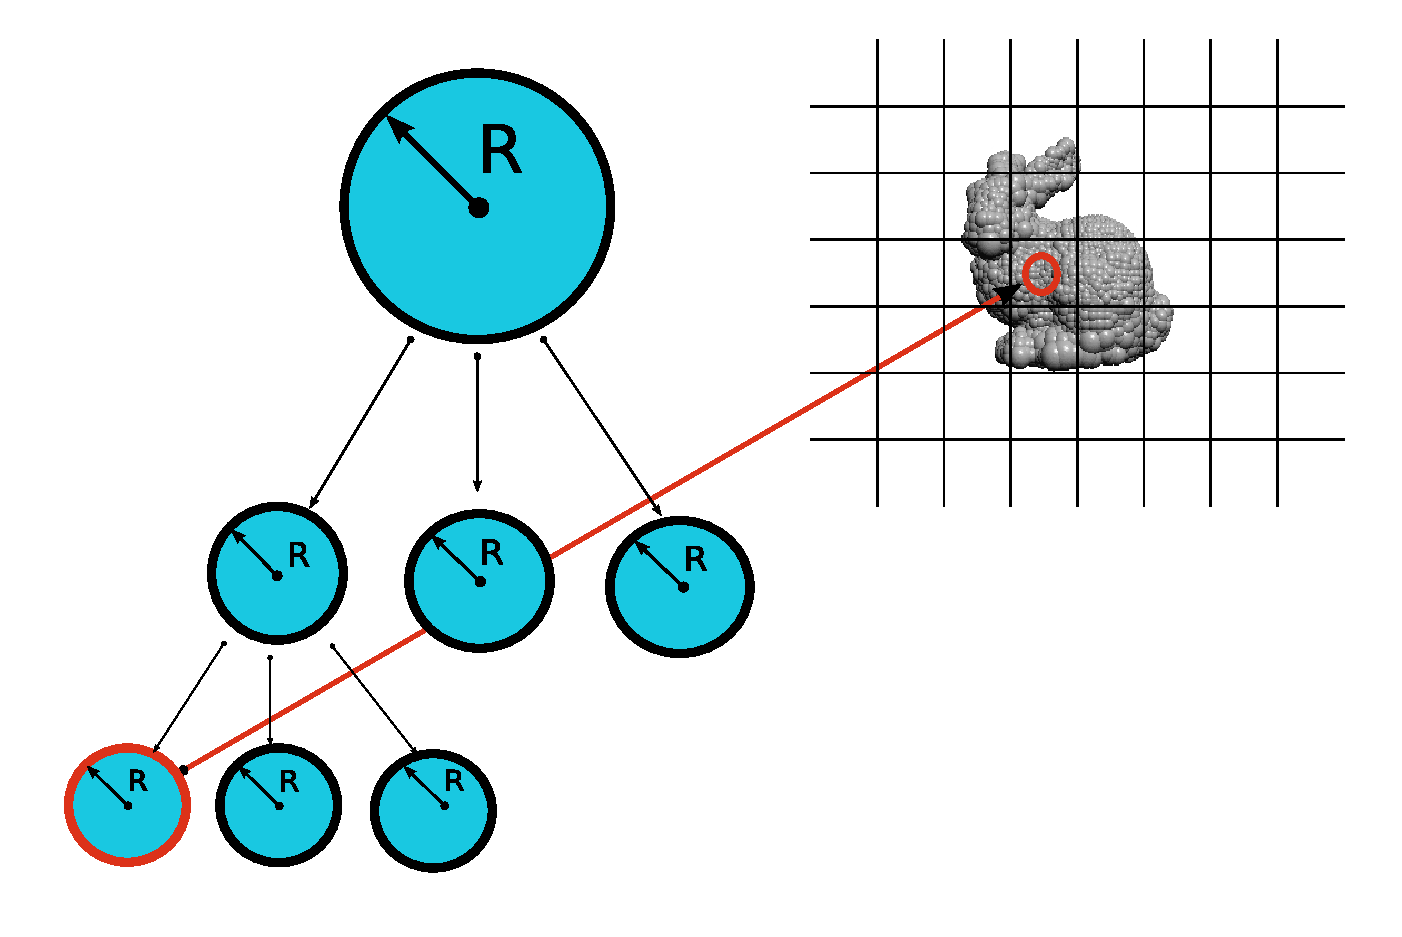
\includegraphics[width=1.25\linewidth]{img/cap02/CoelhoRender}\\[0cm](b)
  \end{minipage}
  \hfill \mbox{}
  \caption{\label{fig:percorrimento}Esquema do algoritmo de renderiza��o:  
  \emph{(a)} Tamanho da imagem projetada do n� � maior que um \textit{pixel}.
  Continua o percurso nas sub-�rvores; \emph{(b)} Tamanho da imagem
  projetada do n� � menor que um \textit{pixel}. Renderiza o \textit{splat}.}
\end{figure}

\subsection{Discuss�o}
\textit{QSplat} possui um processo bem simples, mas infelizmente ele n�o usa
todo o potencial gr�fico que as GPUs oferecem. Dada
granularidade na sua determina��o de n�vel de detalhes, um modelo chega e ser
renderizado ponto por ponto. Como consequ�ncia, esse ``modo imediato'' de
renderizar torna a GPU pouco utilizada, pois est� sempre esperando
por novos dados para renderizar. Levando em conta que n�o � apenas a coordenada
de um ponto que est� sendo utilizada, mas todos os seus outros atributos, como
cor e normal.

No entanto, est� simplicidade torna o \textit{Qsplat} um algoritmo que pode ser
usado em outras aplica��es. Sua hierarquia de esfera � uma boa estrutura para
\textit{Ray Tracing}. Outra s�o aplica��es em rede como a do \textit{Stream
QSplat}\cite{Rusinkiewicz2001} que permite visualizar modelos $3D$ de forma
progressiva e remotamente.


\section{\textit{Sequential Point Trees}}
\textit{QSplat} possui um processamento de dados muito simples e de f�cil
implementa��o, mas infelizmente sua estrutura hier�rquica recursiva � dif�cil de
ser implementada em GPU. Os pontos renderizados n�o s�o armazenados de forma
cont�nua, portanto n�o s�o processados sequencialmente.A \textit{CPU}
(\textit{Central Processor Unit})%
\abbrev{CPU}{\textit{Central Processor Unit}} percorre a
�rvore e faz chamadas independentes para renderizar cada n�. Isso causa um
``gargalo'' entra a CPU e a GPU, sendo que esta �ltima fica muito tempo ociosa
esperando por dados da CPU.
\textit{Sequential Point Trees} prop�e o uso da estrutura de \textit{QSplat},
s� que de uma forma sequencial que � facilmente tratada em GPU. Sendo assim,
transferindo mais trabalho para GPU e diminuindo este ``gargalo''.
Nas se��es que seguem , SPT ser� apresentado com mais detalhes. 
\subsection{Hierarquia de Pontos}
Inicialmente SPT possui um hierarquia de pontos representada por um
\textit{Octree} \cite{Samet05}. Cada n� da hierarquia representa parte do
objeto. Ela armazena um centro \textbf{c} e uma estimativa da normal
\textbf{n}. Um n� armazena tamb�m um di�metro \textbf{d} da esfera envolvente
centrada em \textbf{c}. O n� interior representa
a uni�o de seus n�s filhos, ent�o o di�metro cresce a medida que sobe na
hierarquia. Os n�s folhas possuem pontos que s�o distribu�dos uniformemente no
objeto, ent�o possuem di�metro aproximadamente iguais.

\subsection{M�tricas de Erro}

Cada n� na hierarquia pode ser aproximada por um disco com o mesmo centro,
normal e di�metro do n�. O erro dessa aproxima��o � descrito por dois valores
: o erro perpendicular $e_p$ e o erro tangencial $e_t$.
 
\noindent \textbf{Erro Perpendicular:}
O erro perpendicular $e_p$ � a dist�ncia m�nima entre dois planos
paralelo ao disco que engloba todos os filhos. Este erro mede vari�ncia e pode ser
calculado como:

\begin{figure}[tcb]
  \centering \mbox{} \hfill
  \begin{minipage}[b]{0.40\linewidth}
 \centering
 
  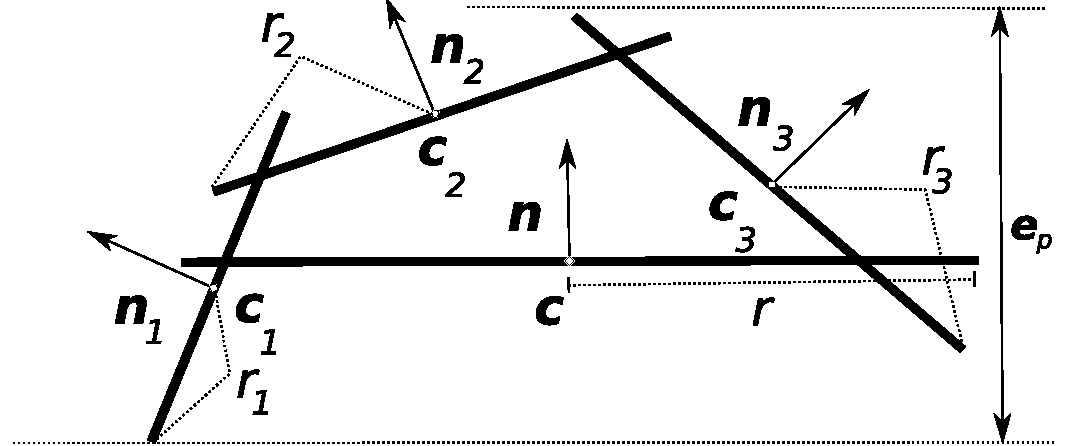
\includegraphics[width=1.0\linewidth]{img/cap02/PosterSquential}
  \end{minipage}
  \hfill
  \begin{minipage}[b]{0.40\linewidth}
    \centering
    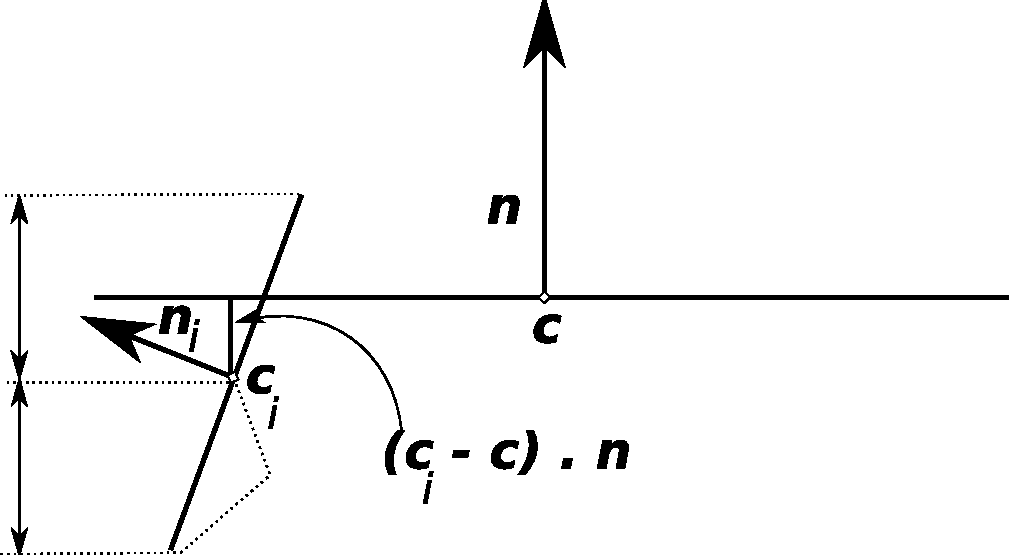
\includegraphics[width=1.0\linewidth]{img/cap02/di}
  \end{minipage}
  \hfill \mbox{}
  \caption{\label{fig:perpendicular}Como erro perpendicular, usa-se a
  dist�ncia entre dois plano paralelo ao disco que engloba todos os filhos
  (Retirada de \cite{Dachsbacher2003}).}
\end{figure}

\begin{eqnarray}
 e_p & = & max\{((c_i-c)\cdot n)+d_i\} - min\{((c_i-c)\cdot n )-d_i\} \\
     &   &\textnormal{with}\hspace{0.5cm}  d_i = r_i \sqrt{1-(n_i\cdot n)^2}
  \label{perpendicular}
\end{eqnarray}

Durante a renderiza��o, o erro perpendicular � projetado na imagem, resultando
em um erro $\tilde{e}_p$. $\tilde{e}_p$ � proporcional ao seno do �ngulo entre
o vetor de vis�o $v$ e a normal do disco $n$ e diminui com $\cfrac{1}{r}$ e $r =
|v|\cdot\tilde{e}_p$ captura erros ao longo das silhuetas:
 
 \begin{equation}
  \tilde{e}_p  = e_p \frac{\sin{(\alpha)}}{r} \quad \text{sendo} \quad \alpha =
  \angle(n,v)
   \label{tangencial}
 \end{equation}

\noindent \textbf{Erro Tangencial:}
O erro tangencial $e_t$, analisa a proje��o dos discos dos filhos no
disco do pai como mostrado na Figura \ref{fig:Tangencial}. $e_t$ mede se o
disco pai cobre um grande �rea desnecess�ria. O erro � medido usando v�rias
retas ao redor dos filhos projetados. $e_t$ � portanto o menor di�metro do
disco pai menos o tamanho do menor intervalo entre retas. (d�vida em rela��o a
escrita). $e_t$ negativos s�o setados em zero. $e_t$ � projetado no espa�o de
imagem como:

\begin{equation}
 \tilde{e}_t = e_t \frac{\cos{(\alpha)}}{r} 
  \label{tangencial}
\end{equation}

\noindent \textbf{Erro Geom�trico:}
O erro perpendicular e tangencial podem ser combinados em um �nico erro
geom�trico:
Agora o erro no espa�o de imagem $\tilde{e}_g$ depende apenas de $r$, e n�o mais
do �ngulo do vis�o: $ \tilde{e}_g = \cfrac{e_g}{r}$
 
 \begin{equation}
 \tilde{e}_g  = \max\{e_p\sin{\alpha} + e_t\cos{\alpha}\} = \sqrt{e^2_p + e^2_t} 
  \label{tangencial}
\end{equation}

\begin{figure}[ht]
\centering
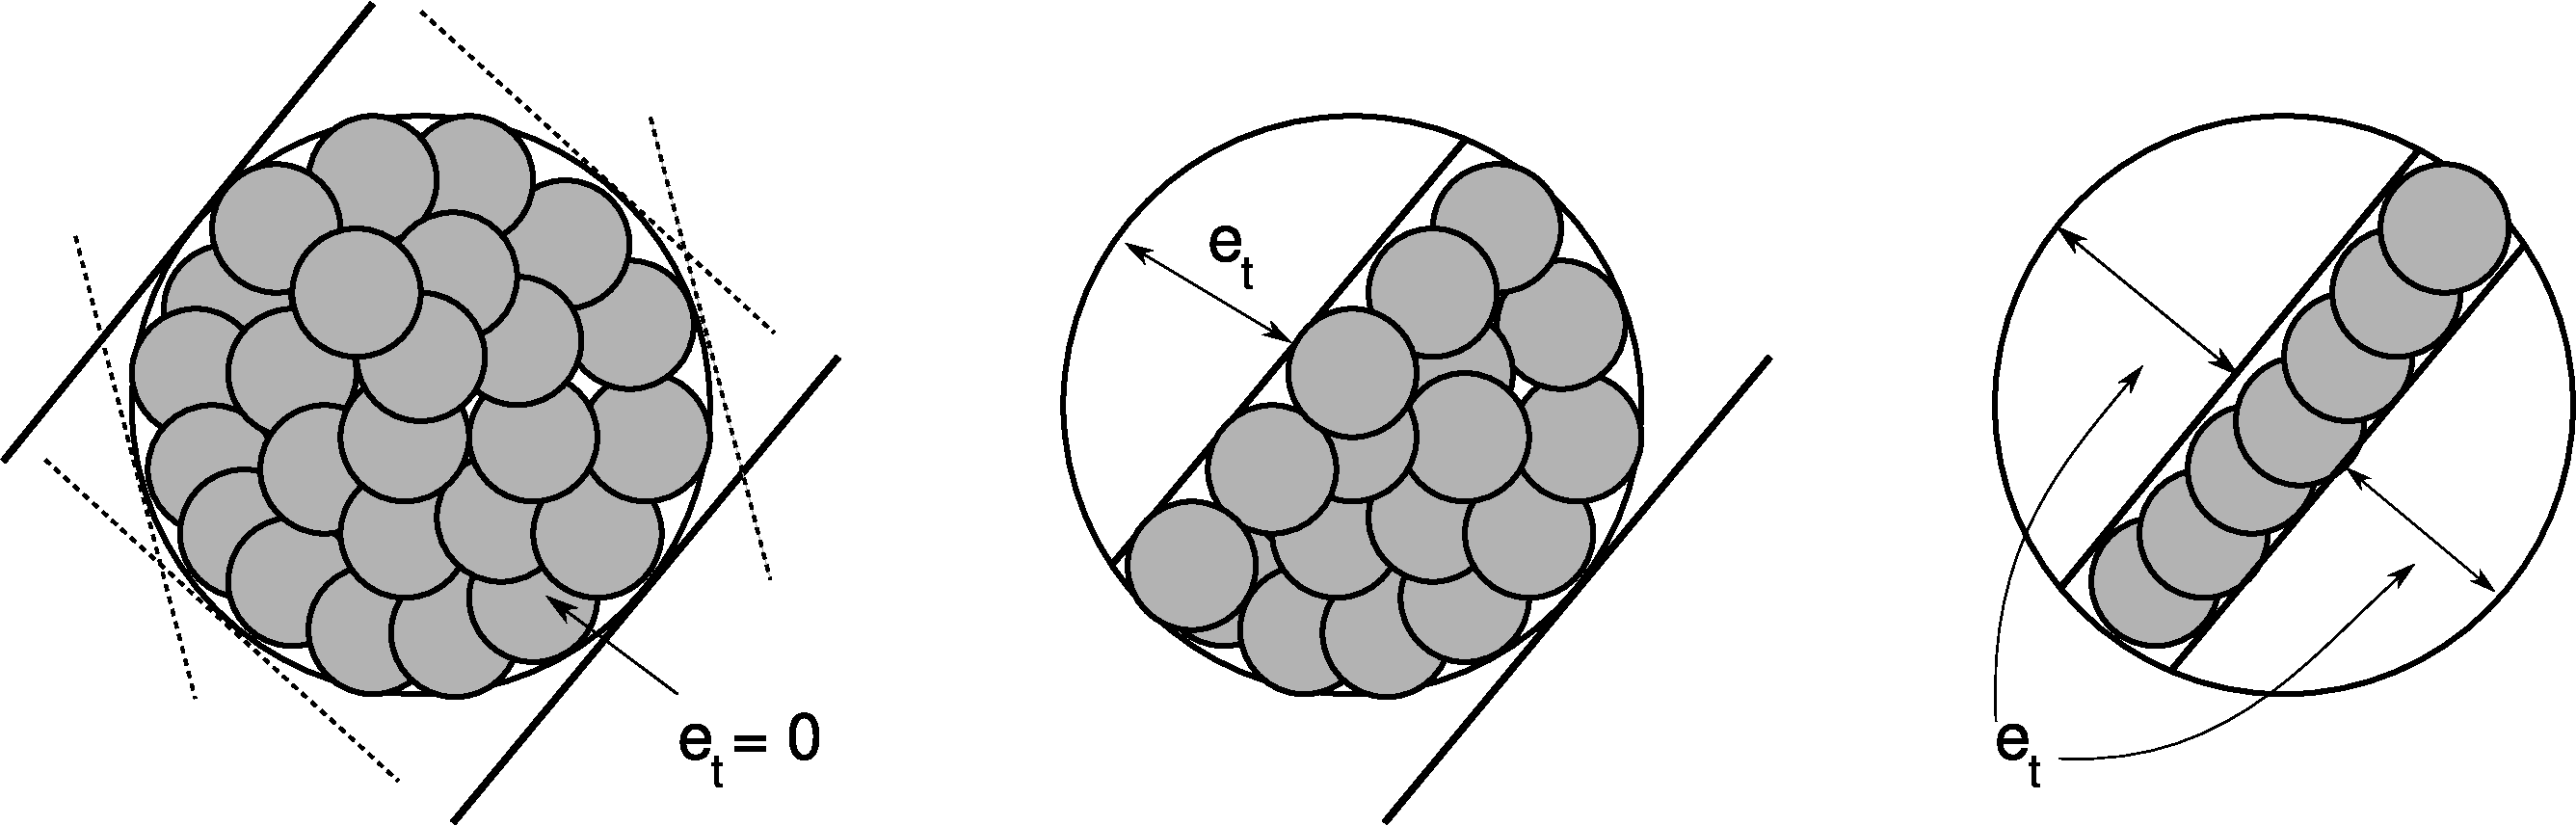
\includegraphics[width=15.0cm]{img/cap02/tangencial} 
\caption{Erro tangencial, mede o qu�o aproximado � o disco pai em rela��o ao
filho no plano tangente (Retirada de \cite{Dachsbacher2003}) .}
\label{fig:Tangencial}
\end{figure}

\subsection{Renderiza��o Recursiva}
Um objeto � renderizado na hierarquia de pontos usando um percurso em
profundidade. Para cada n� um erro de imagem $\tilde{e}_g$ � calculado. Se
$\tilde{e}_g$ est� abaixo de um limite de erro estabelecido $\epsilon$ e o n�
n�o � uma n� folha , seus filhos s�o percorridos recursivamente. Por outro lado,
um \textit{splat} de tamanho $\tilde{d} =  d/r$ � renderizado. Note que
esta hierarquia de pontos n�o se adapta apenas a dist�ncia do observador $r$,
mas tamb�m para propriedades da superf�cie. Grandes �reas planas s�o detecta-das
com pequenos erro geom�trico $\tilde{e}_g$ e podem ser renderizados com splats
grandes.
\subsection{Arranjamento}
O procedimento de renderiza��o da se��o anterior � recursivo e n�o se adapta ao
processamento r�pido e sequ�ncial da GPU. Assim, h� um arranjamento da
estrutura em �rvore para um estrutura em lista e o teste recursivo �
substitu�do por um percurso sequ�ncial sobre a lista de pontos.

Para isso, o erro simplificado $\tilde{e}_g$ � substitu�do por um que sejam
mais intuitivo. Assume-se que $\epsilon$ � constante. O teste
recursivo � $\tilde{e}_g = {e}_g/r < \epsilon $ e ao inv�s de $e_g$, �
armazenado um dist�ncia m�nima $r_{\min} = e_g/ \epsilon$ que simplifica o
teste recursivo para $r > r_{\min}$. Entretanto, quando os n�s da �rvore s�o
processados seq�encialmente sem informa��o hier�rquica, h� necessidade de um
teste n�o recursivo. Para esse fim, � adicionado um par�metro $r_{\max}$, que �
simplesmente um $r_{\min}$ do seu n� pai, em cada n� e usa-se $r \in
[r_{\min},r_{\max}]$ como um teste n�o recursivo. Desta maneira pode-se guiar o
algoritmo de renderiza��o com esse teste \textit{intercalar} para cada n�.

\begin{figure}[tcb]
  \centering \mbox{} \hfill
  \begin{minipage}[b]{0.40\linewidth}
 \centering
  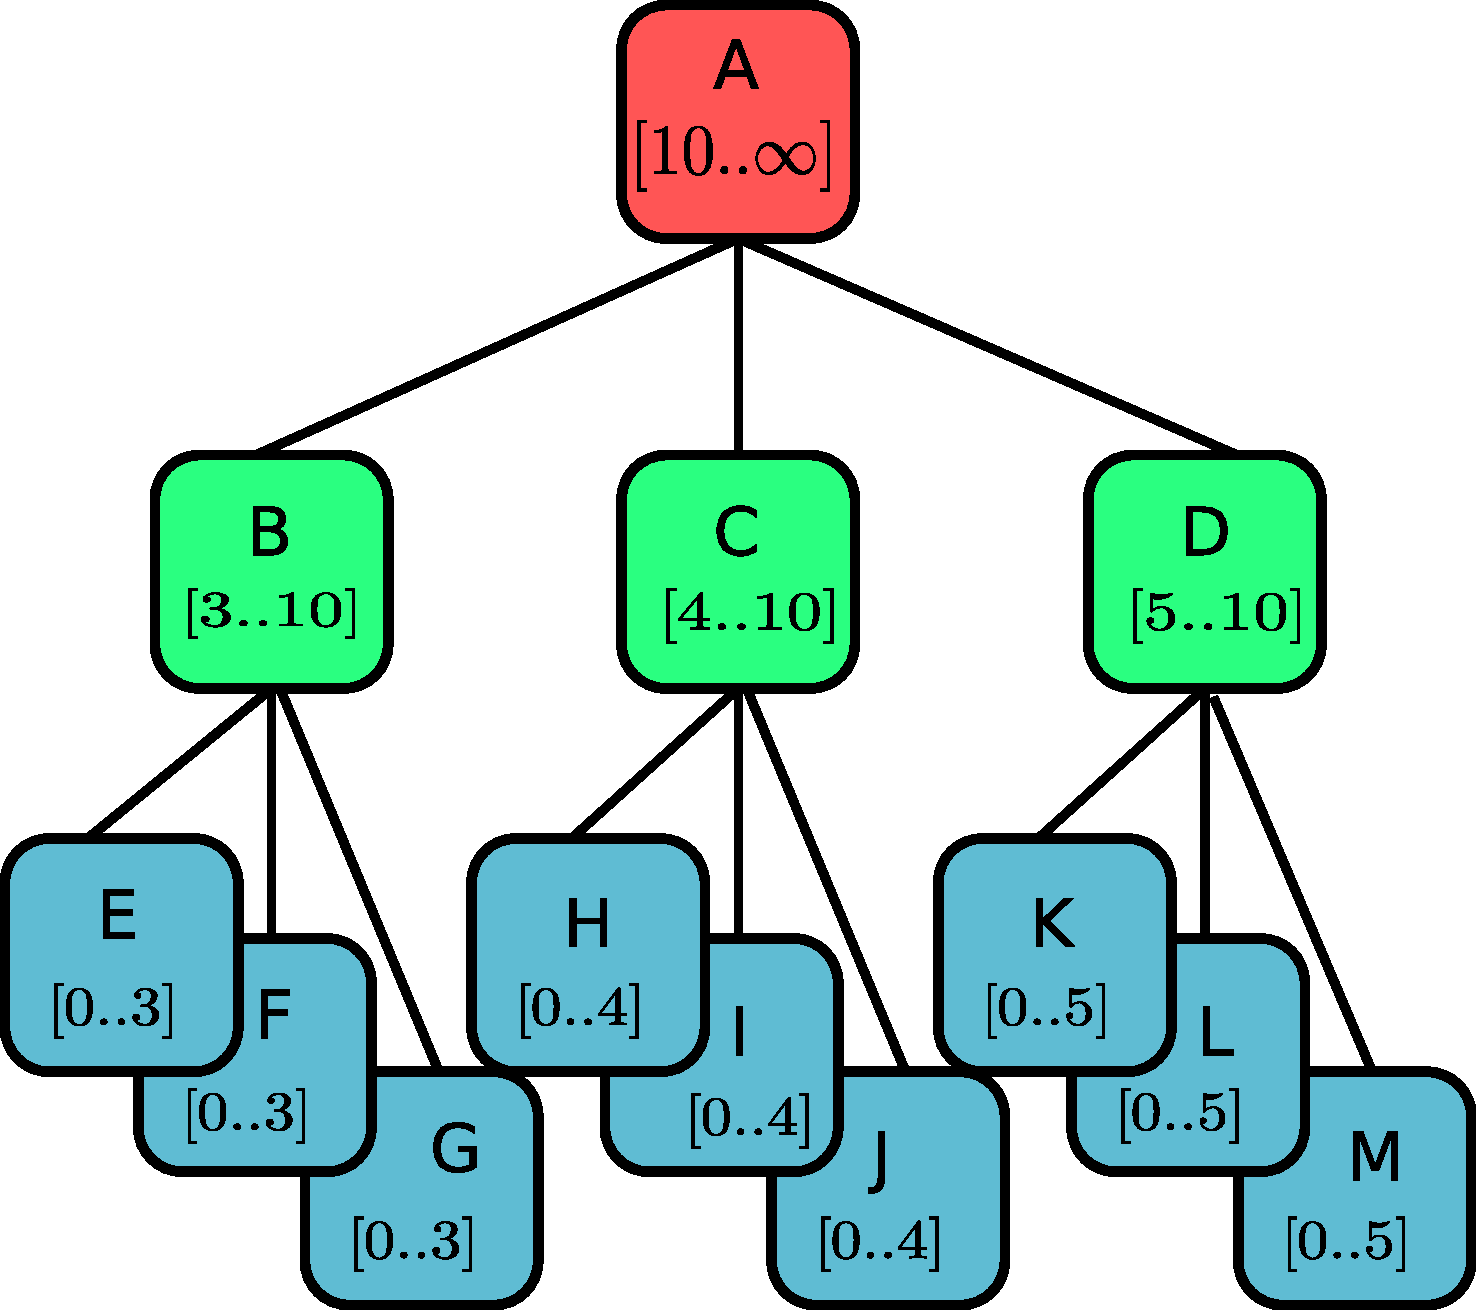
\includegraphics[width=1.0\linewidth]{img/cap02/SequentialTree}\\[0cm](a)
  \end{minipage}
  \hfill
  \begin{minipage}[b]{0.40\linewidth}
    \centering
    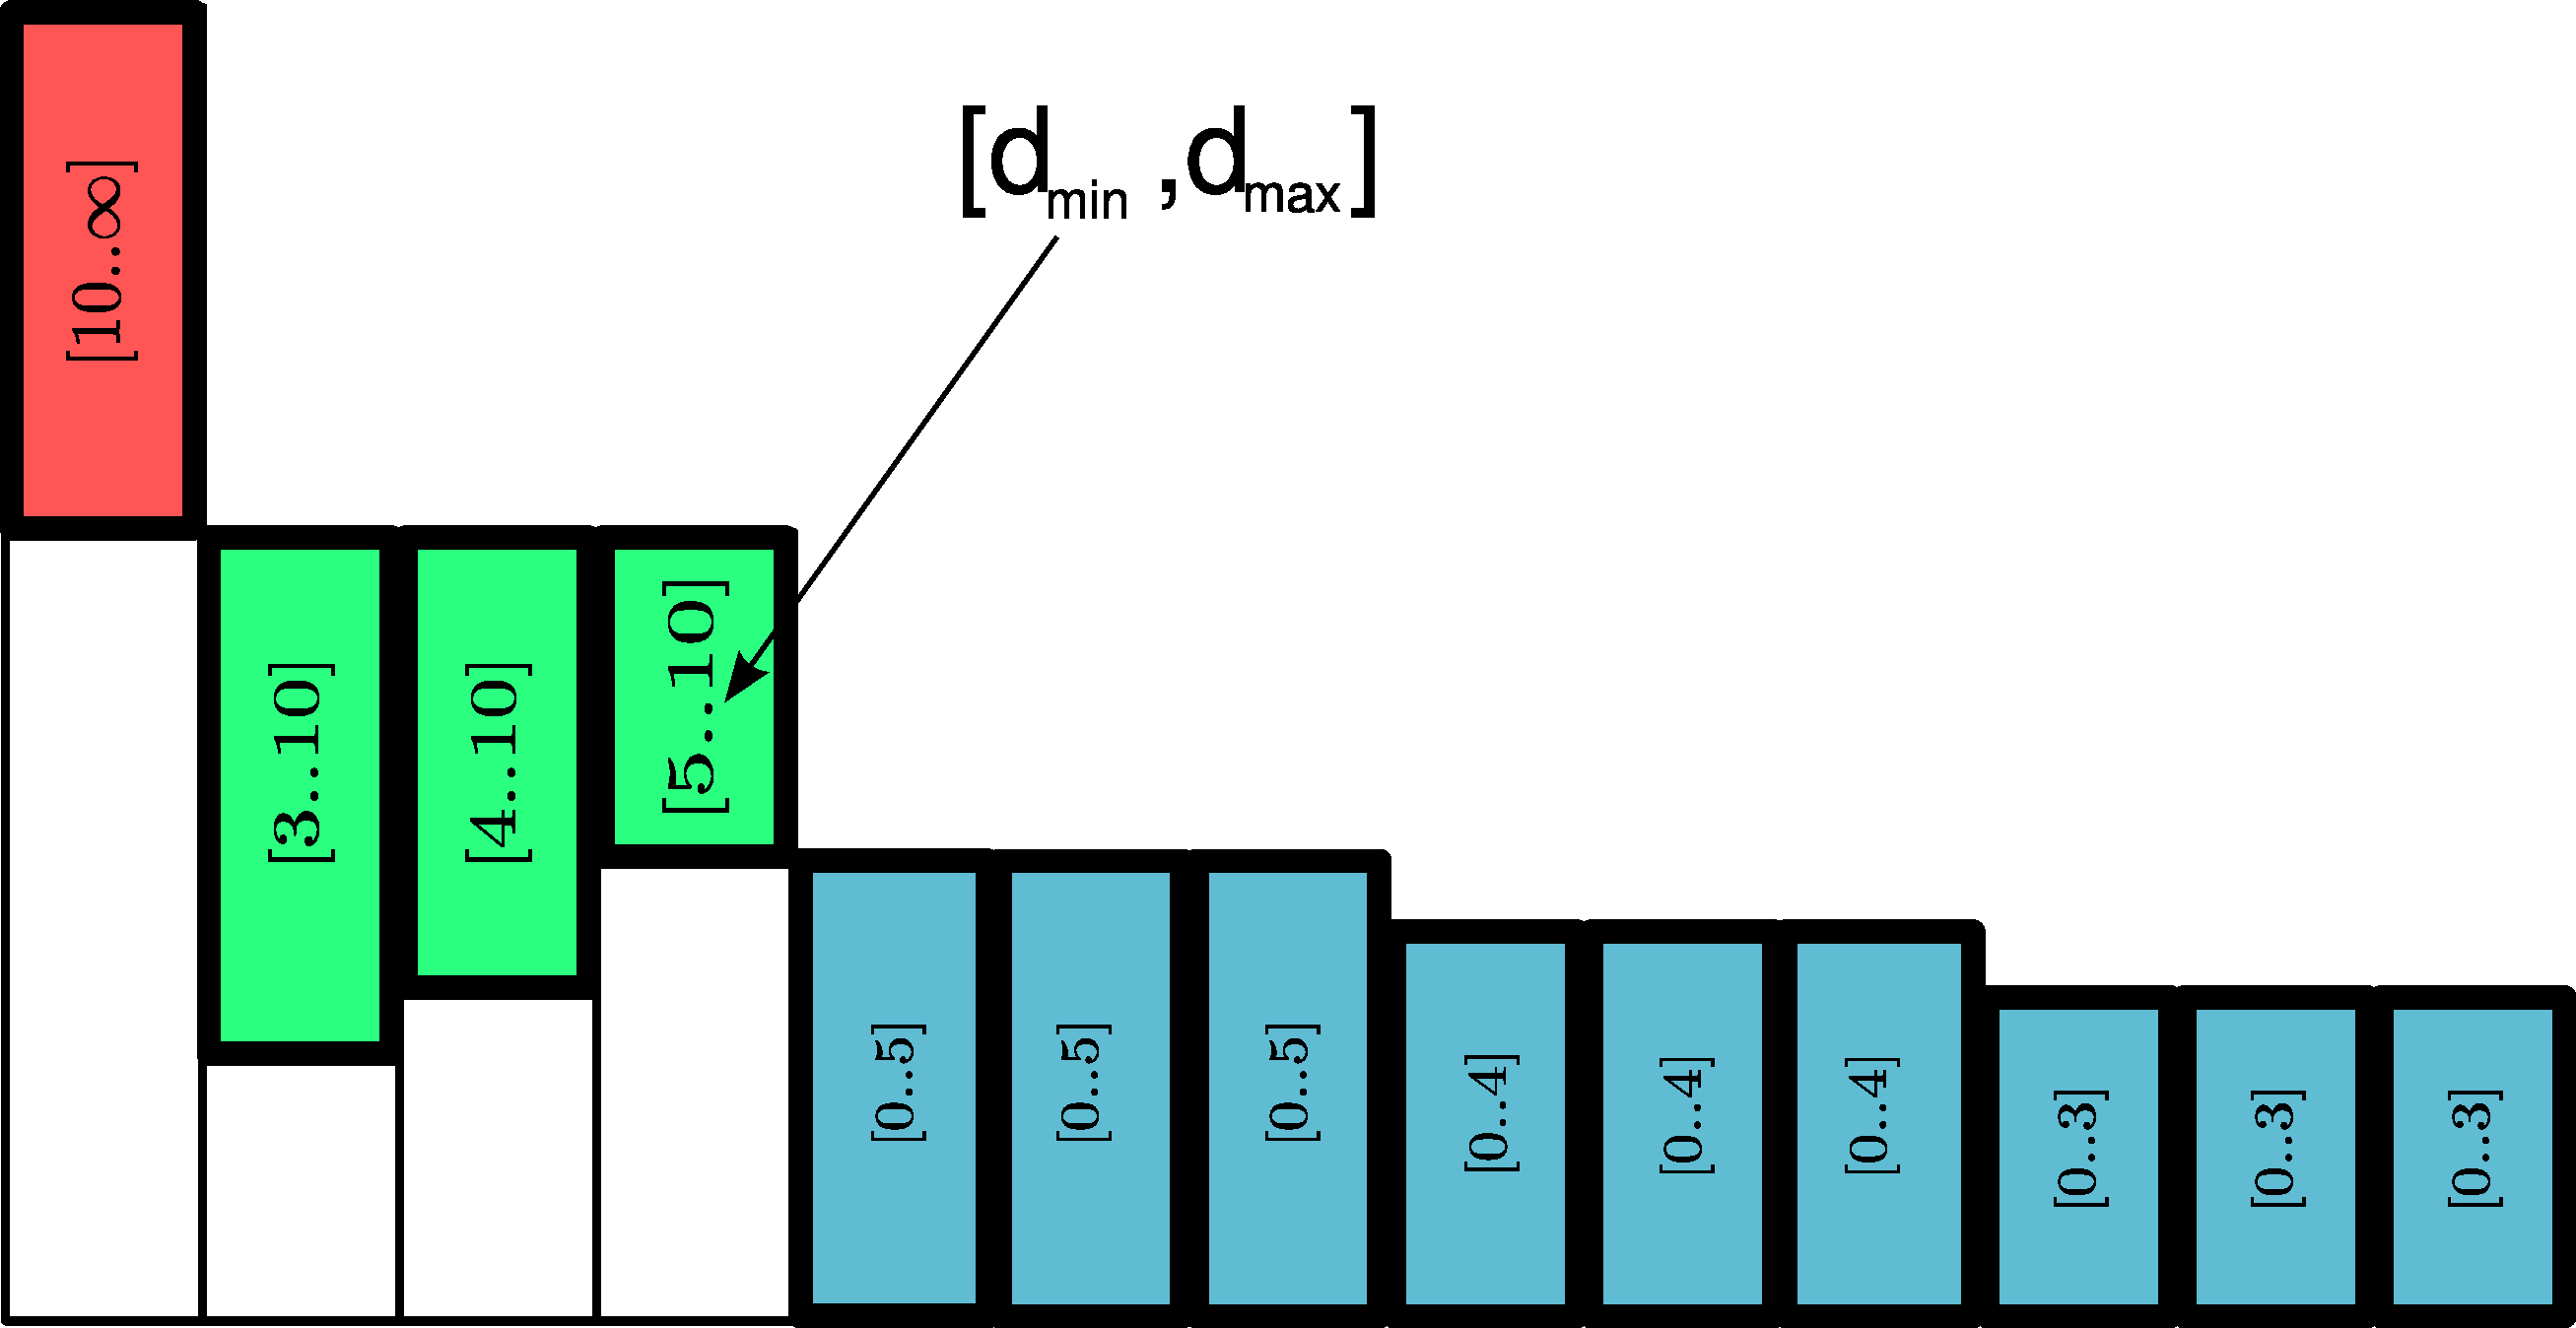
\includegraphics[width=1.2\linewidth]{img/cap02/SequentialDamx}\\[0cm](b)
  \end{minipage}
  \hfill \mbox{}
  \caption{\label{fig:list}Como erro perpendicular, usa-se a
  dist�ncia entre dois planos paralelos ao disco que engloba todos os filhos
  (adaptada de \cite{Dachsbacher2003}).}
\end{figure}


Depois de substituir o teste recursivo por um simples teste intervalar, a
hierarquia de pontos e transformada em um lista, que � processada
sequencialmente. Neste est�gio, $[r_{\min},r_{\max}]$ � usada para ordenar a
lista de forma decrescente a partir de $r_{\max}]$ como ilustrado na
Figura \ref{fig:list}.

Um exemplo de como o algoritmo de renderiza��o funciona � mostrado na Figura
\cite{fig:SequentialList}. Onde para diferentes valores de $r$ um por��o da
lista � selecionada enquanto outras s�o descartadas.

\begin{figure}[ht]
\centering
\includegraphics[width=15.0cm]{img/cap02/SequentialList} 
\caption{(Retirada de \cite{Dachsbacher2003}) .}
\label{fig:SequentialList}
\end{figure}

\subsection{Discuss�o}

SPT � simples, de f�cil implementa��o e prov� um renderiza��o continua usando
n�vel de detalhes.

O autor da �nfase no fato de que grande parte do trabalho � movido para GPU,
deixando a CPU livre para outras tarefas. No entanto, SPT s� � eficiente se o modelo 
estiver na mem�ria de v�deo, o que nem sempre � poss�vel.

SPT renderiza pontos em baixa qualidade, j� que a GPU n�o suporta renderizar
\textit{splat} com qualidade em tempo satisfat�rio. Outra desvantagem � que SPT
n�o realiza \textit{frustum culling}, perdendo o pouco em efici�ncia.







%\section{Clusteriza��o}
%M�todos de clusteriza��o tem sido usados em computa��o gr�fica para reduzir a
%complexidade de modelos 3D. Por Exemplo Rossignac and Borrel em seu trabalho
%pioneiro \cite{Rossignac1992}, usaram clusteriza��o de v�rtices para obter
%uma multi-resolu��o aproximada de modelos poligonais complexos para torna 
%renderiza��o mais eficiente\cite{Rossignac1992}. As abordagens de constru��o 
%de clusters s�o categorizadas em incremental (\textit{bottom-up}) e o
%hier�rquico (\textit{top-down}). O modo incremental os clusters s�o criado
%juntando-se uma ou mais amostras em um cluster apropriado. Enquanto o modo
%hier�rquico incia com um cluster de todas as amostras e recursivamente
%separa-os em clusters menores apropriados.
%Os dois grandes desafios da clusteriza��o s�o estabelecer a medida de
%similaridade (caso incremental) ou dissimilaridade (caso hierarquico)
%empregada e definir o n�mero final de clusters.
%Abaixo ser�o aprenstados m�todos de clusteriza��o que foram usados tanto em
%simplifica��o como para multi-resolu��o em modelos baseados em pontos.
%A estrat�gia usada por Rossignac and Borrel
%\cite{Rossignac1992} foi envolver o modelo em uma grade regular (veja
%\ref{2:gradeRegular}) e sub-dividi-l�. A resolu��o da grade regular
%determinava a qualidade da simplifica��o. Essa abordagem volum�trica possui
%uma desvantagem. Usando-se uma grade com c�lulas de tamanho fixo, esse m�todo
%n�o se adapta bem a modelos que n�o apresentam um distribui��o espacial
%uniforme. Para evitar essa (  ), um clusteriza��o baseada na superf�cie pode
%se usada onde os clusters s�o constru�dos pela sele��o de amostras na sua
%vizinhan�a. Estas t�cnicas ser�o apresentadas a seguir.
%\subsection{Clusteriza��o Hier�rquica}
%Para construir um multiresolu��o de modelos baseados em pontos, muitos autores
%[v�rios] tem adotado alguma estrat�gia de parti��o do espa�o com o intuito de 
%visualiza��o de modelos complexos eficientemente. Nesta se��o discutiremos as
%estrutura de parti��o espacial Octree, BSP Tree e Hierarquia de Esferas
%Envolventes.
%Para mais detalhes de
%compara��o ver \cite{Samet2005}


  \chapter{Simplifica��o de Superf�cies}
Como mencionado no cap�tulo \ref{cap:02}, modelos baseados em pontos complexos podem chegar a
milh�es ou mesmo bilh�es de amostras, como por exemplo no projeto do David Digital\cite{Levoy2000}. 
Para que seja poss�vel processar ou visualizar estes modelos em tempo real, muitas vezes � necess�rio reduzir a complexidade realizando opera��es de simplifica��o.
Estas t�cnicas geram aproxima��es adequadas do modelo reduzindo o n�mero de amostras e procurando manter da melhor forma poss�vel as caracter�sticas do modelo original.
Formalmente, o objetivo de uma simplifica��o de superf�cies baseadas em pontos
pode ser formuladas da seguinte forma: 

Seja uma superf�cie $\mathbf{\mathcal{S}}$
definida por uma nuvem de pontos $\mathbf{\mathcal{P}}$. Dado um n�mero
amostras $n < |\mathbf{\mathcal{P}}|$, compute uma nuvem de pontos
$\mathbf{\mathcal{P}}^\prime$, onde $|\mathbf{\mathcal{P}^}^\prime| = n$, tal que
a dist�ncia $\mathbf{\varepsilon} =
\mathbf{\mathit{d}}(\mathbf{\mathcal{S}},\mathbf{\mathcal{S}}^\prime)$ da
superf�cie simplificada $\mathbf{\mathcal{S}}^\prime$ da superf�cie original 
$\mathbf{\mathcal{S}}$ seja m�nima.

%Na pr�tica ,  achar um �timo global do problema descrito acima � $np - hard$
Diversos algoritmos de simplifica��o utilizam
diferentes heur�sticas baseadas em erros locais para encontrar a melhor aproxima��o.
Neste cap�tulos ser�o apresentados alguns m�todos de simplifica��o divididos em duas categorias:
superf�cies baseadas em pontos \textit{Puros} e baseadas em \textit{Splats}.

%{New point based simplification based on MLS and splat for Point Modesl}

\section{Simplifica��o Baseada em Pontos \textit{Puros}}
\label{sec:puro}
Uma abordagem simples e muito usada na simplifica��o de nuvem de pontos �
avaliar a import�ncia de cada ponto na nuvem de pontos. 
Esta import�ncia � quantificada em um valor que indica a quantidade de informa��o que o ponto possui para formar a superf�cie, ou a sua redund�ncia. 
Linsen \cite{Linsen2001} defini a informa��o contida em um ponto como uma soma ponderada de fatores que inclui dist�ncia e curvatura entre outros, estimados pelos seus vizinhos. 
Em Alexa et al.\cite{Alexa2001} os pontos s�o removidos de acordo com a import�ncia de sua contribui��o
na representa��o da superf�cie dada por \texit{MLS} ( \texit{Moving Least Squares}\abbrev{MLS}{\texit{Moving Least Squares}}).
Kalaiah e Varshney
\cite{Kalaiah2003} medem a import�ncia de cada ponto baseado nas propriedades 
diferenciais fornecidas pela sua vizinhan�a. 
Ap�s a determina��o da import�ncia de cada ponto, a simplifica��o � ent�o realizada removendo os pontos de baixa contribui��o ou alta redunc�ncia. 

\begin{figure}[ht]
\centering
\begin{tabular}{cc}
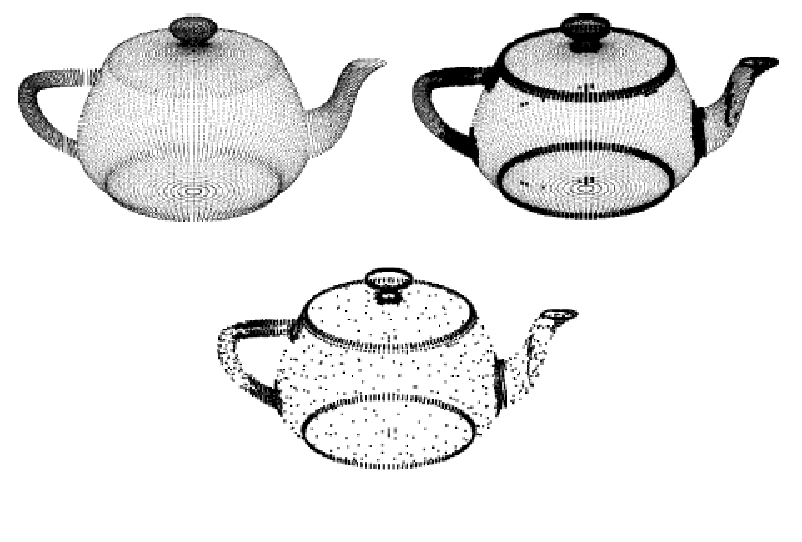
\includegraphics[width=7.0cm]{img/cap04/teaPotSong} &
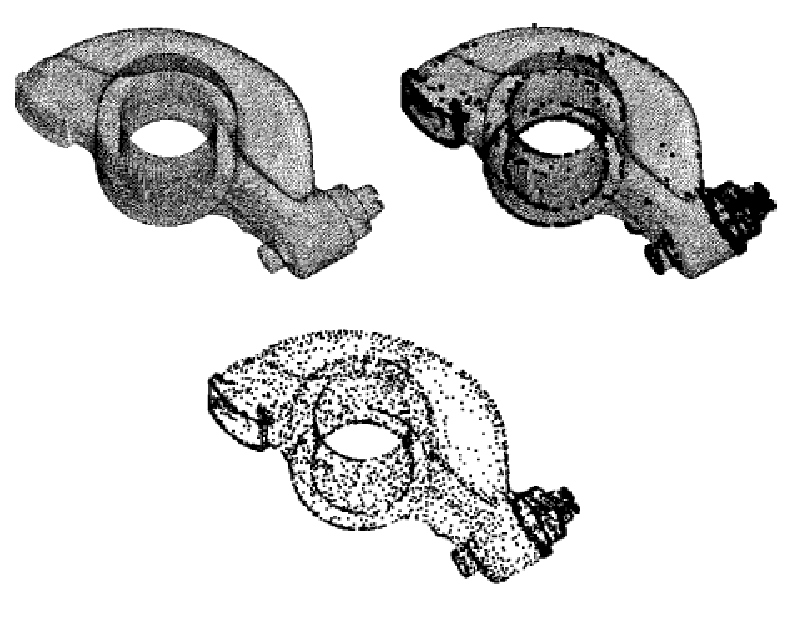
\includegraphics[width=6.0cm]{img/cap04/pecaSong} 
\end{tabular}
\caption{M�todo de simplifica��o proposto por~\cite{Song2009}. Nos dois
modelos: \textbf{Topo-esquerda:} Modelo original. \textbf{Topo-direta:} Em
destaque pontos, classificados como de bordas. \textbf{Baixo:} Modelos
simplificado.}
\label{fig:song2009}
\end{figure}

Os m�todos de simplifica��o citados acima s�o baseados na suposi��o de que a
superf�cie determinada pela nuvem de pontos seja suave. Contudo, alguns modelos, como os de pe�as mec�nicas por exemplo, cont�m descontinuidades, geralmente bordas afiadas que separam a superf�cie em duas
partes distintas. Song e Feng \cite{Song2009} criaram um m�todo de
simplifica��o considerando estes modelos baseado na mesma ideia do m�todos
citados acima, por�m com duas diferen�as principais.
Primeiro, ao inv�s de operar sobre toda a nuvem de pontos de uma s� vez,
o algoritmo considera apenas uma regi�o suave distante por vez. 
Segundo, o grau de import�ncia dos pontos � medido de forma diferente: enquanto Alexa et al.\cite{Alexa2001}
focam em uma simplifica��o
continua, e Kalaiah e Varshney \cite{Kalaiah2003} na renderiza��o e em
uma distribui��o homog�nea, Song e Feng \cite{Song2009} buscam uma simplifica��o
que preserve as partes caracter�stica do modelo, como ilustrado na Figura~\ref{fig:song2009}.

%\begin{figure}[ht]
%\centering
%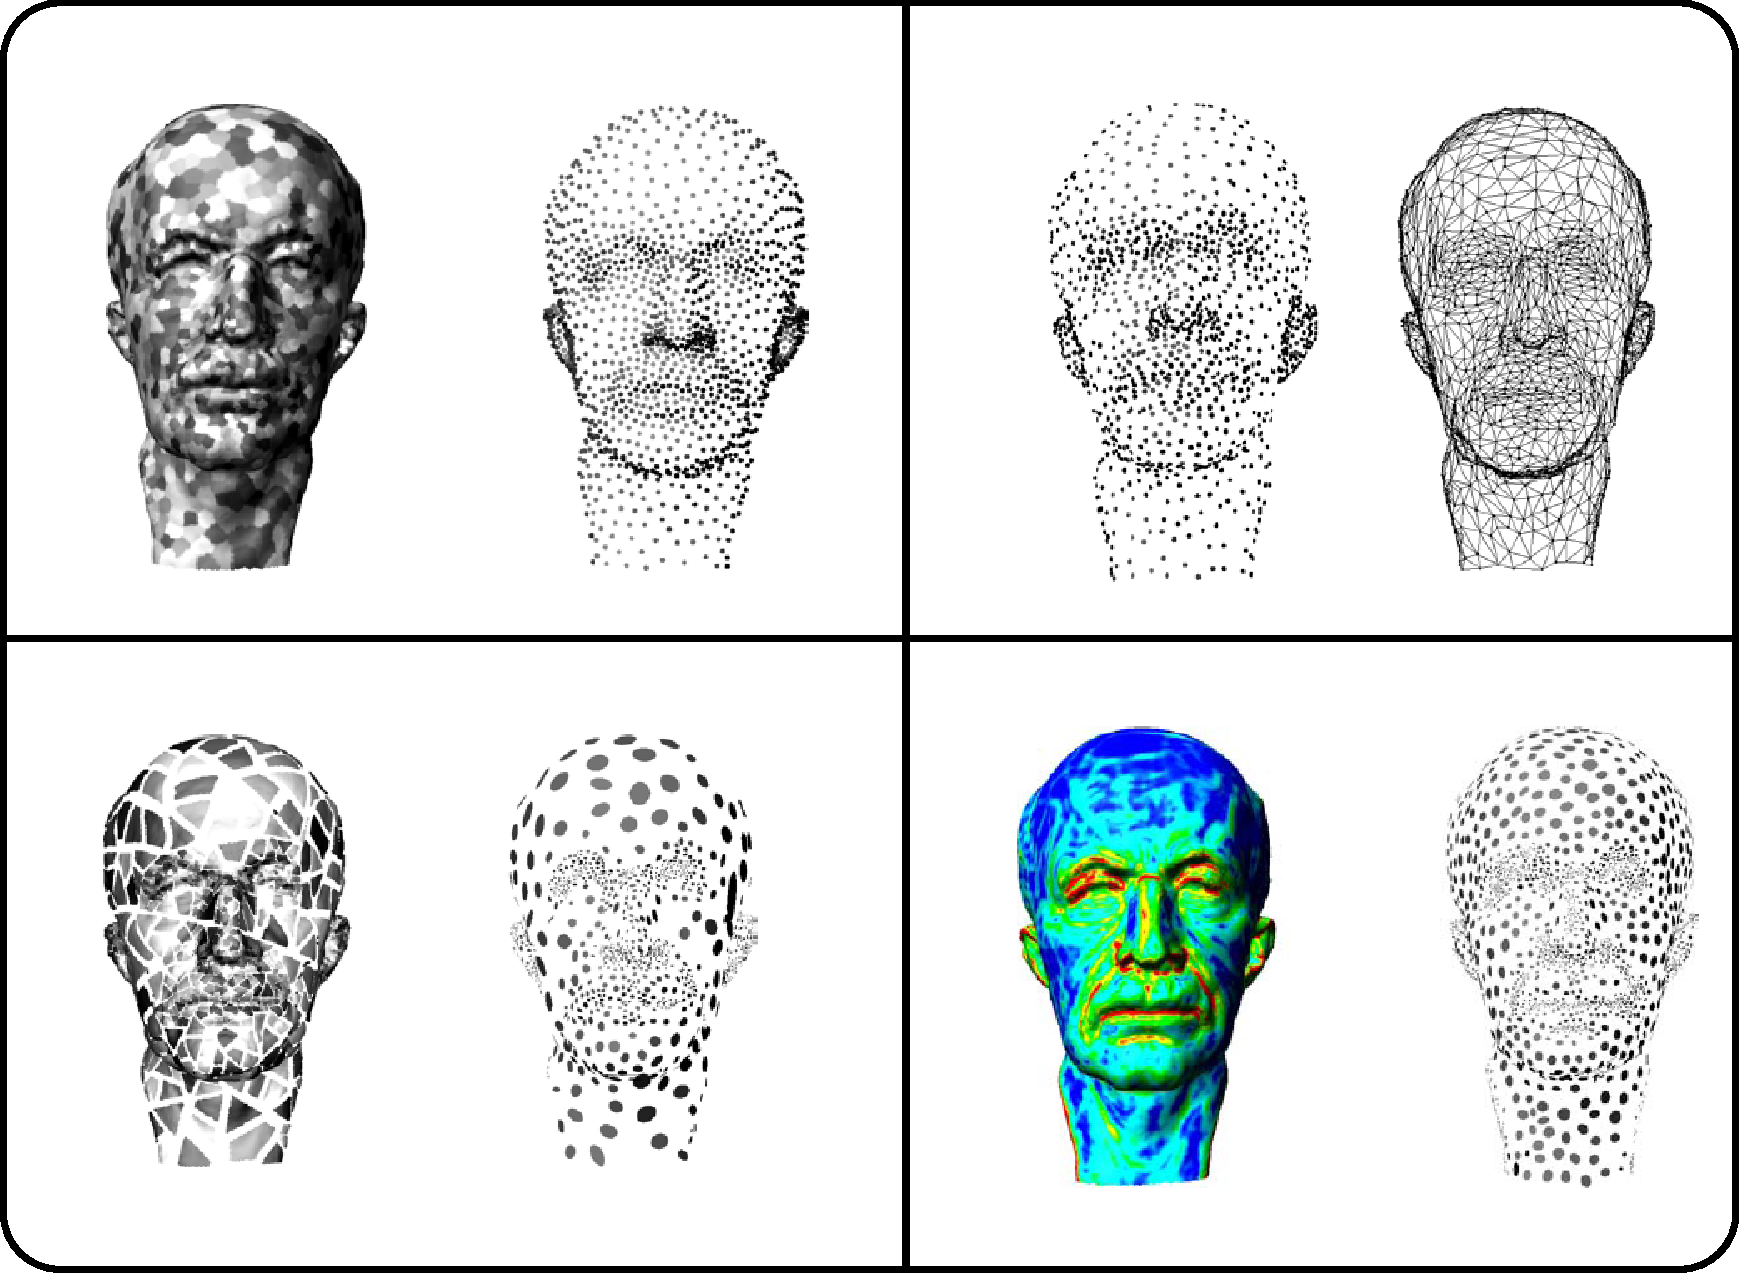
\includegraphics[width=15.0cm]{img/cap04/MaxPlanckPauly} 
%\caption{\textbf{Topo-Esquerda:} \ldots \textbf{Baixo-Esquerda:} \ldots
%\textbf{Topo-Direita:} \ldots \textbf{Baixo-Direta:}}
%\label{fig:maxplanck}
%\end{figure} 



\begin{figure}[ht]
\centering
\begin{tabular}{cc}

	\begin{minipage}[b]{0.45\linewidth}
    	\centering
 	
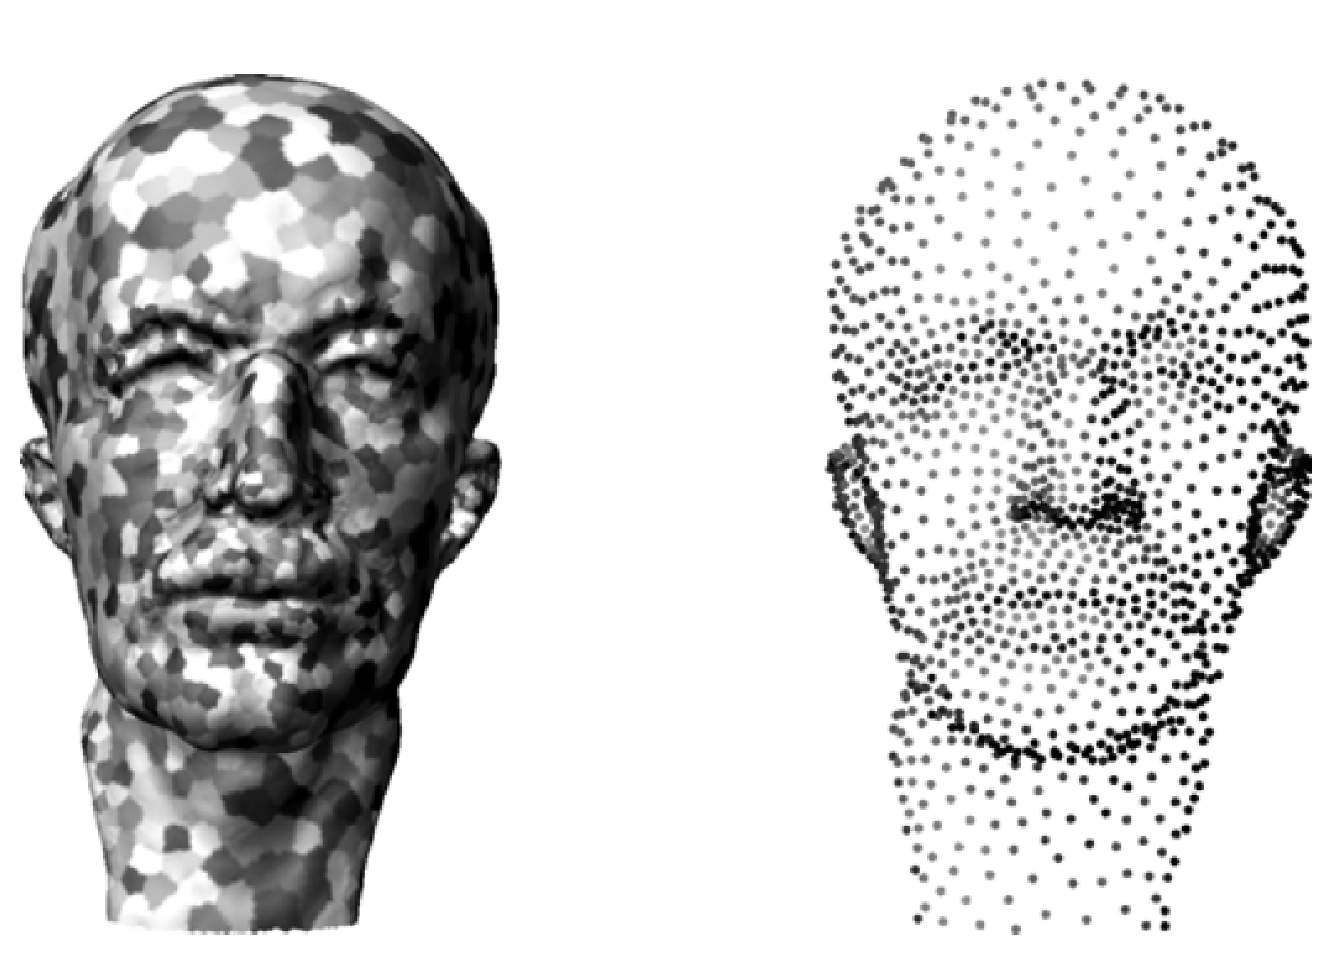
\includegraphics[width=1.00\linewidth]{img/cap04/maxPlanckWinCluster}\\[0cm](a)
   \end{minipage}
   \hfill
   \begin{minipage}[b]{0.45\linewidth}
    	\centering
 	
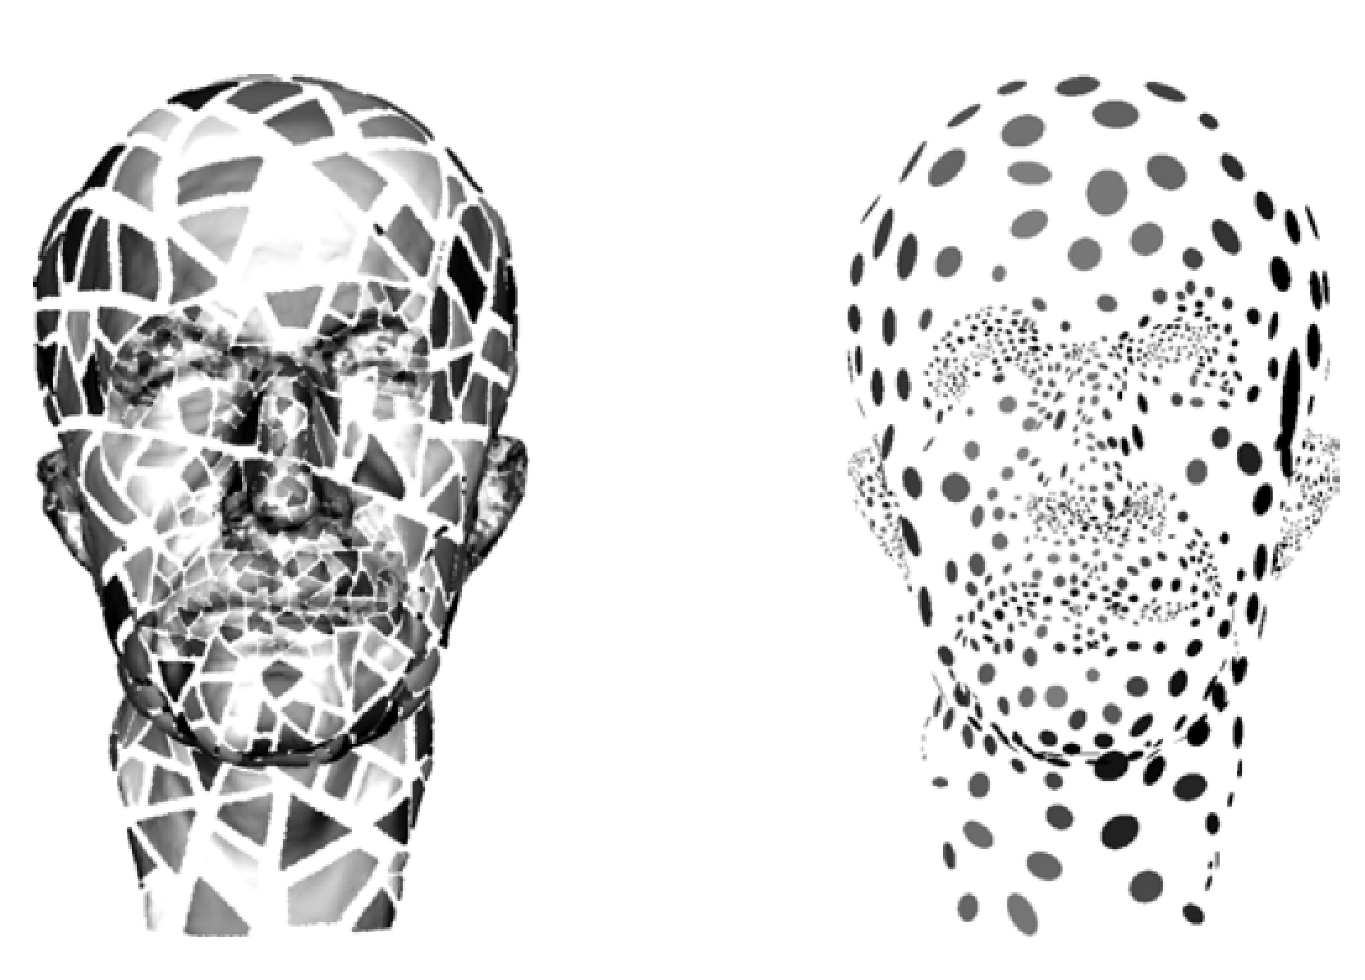
\includegraphics[width=1.00\linewidth]{img/cap04/maxPlanckWinBSP}\\[0cm](b)
   \end{minipage}
	\\
	
  \begin{minipage}[b]{0.45\linewidth}
  		\centering
       
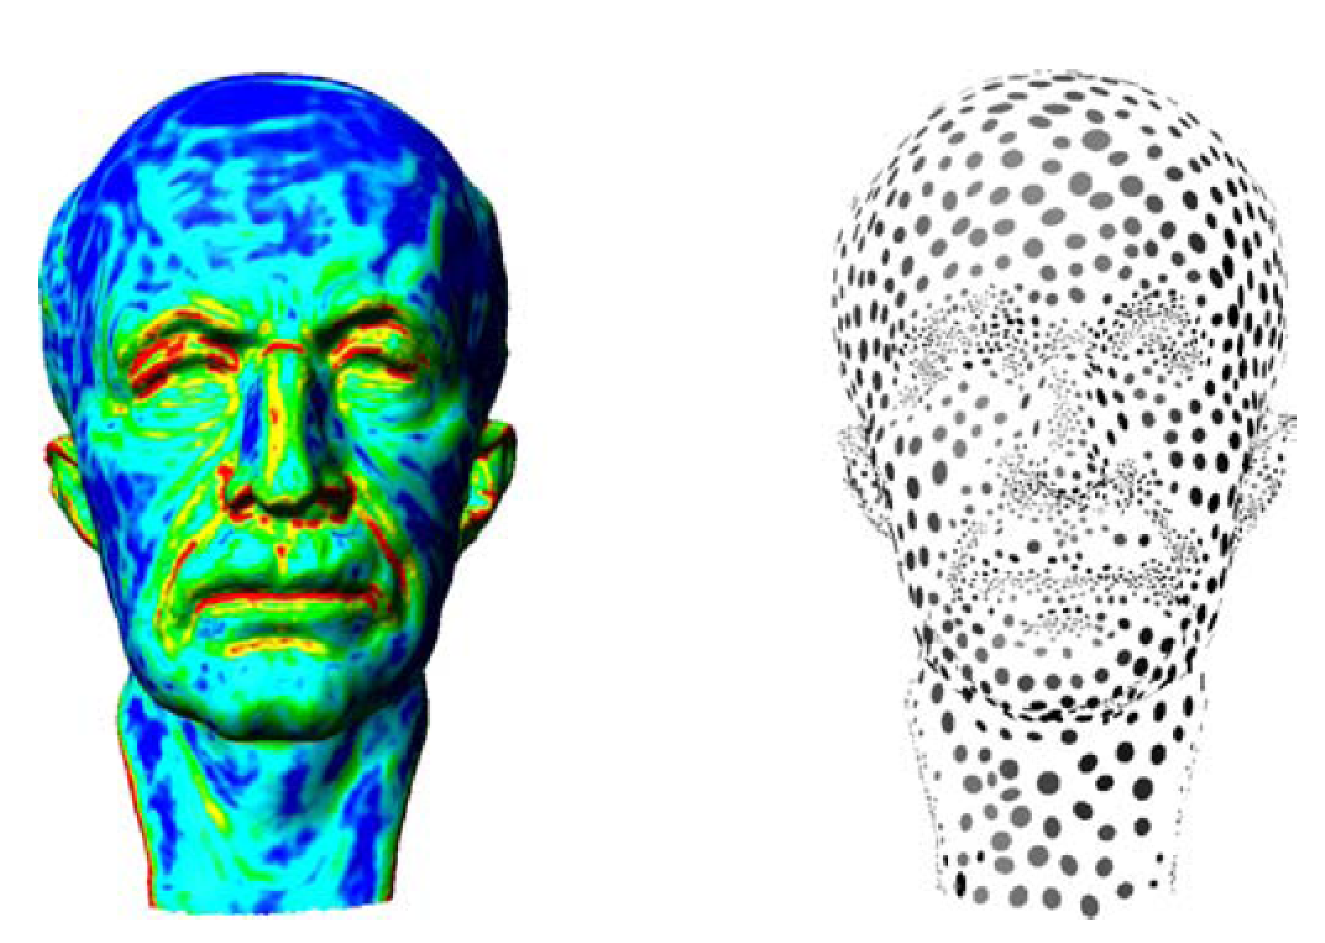
\includegraphics[width=1.00\linewidth]{img/cap04/maxPlanckWinParticulas}\\[0cm]
(c)
  \end{minipage}  
  \hfill
  \centeringmaxPlanckWinCluster
  \begin{minipage}[b]{0.45\linewidth}
    	\centering
       
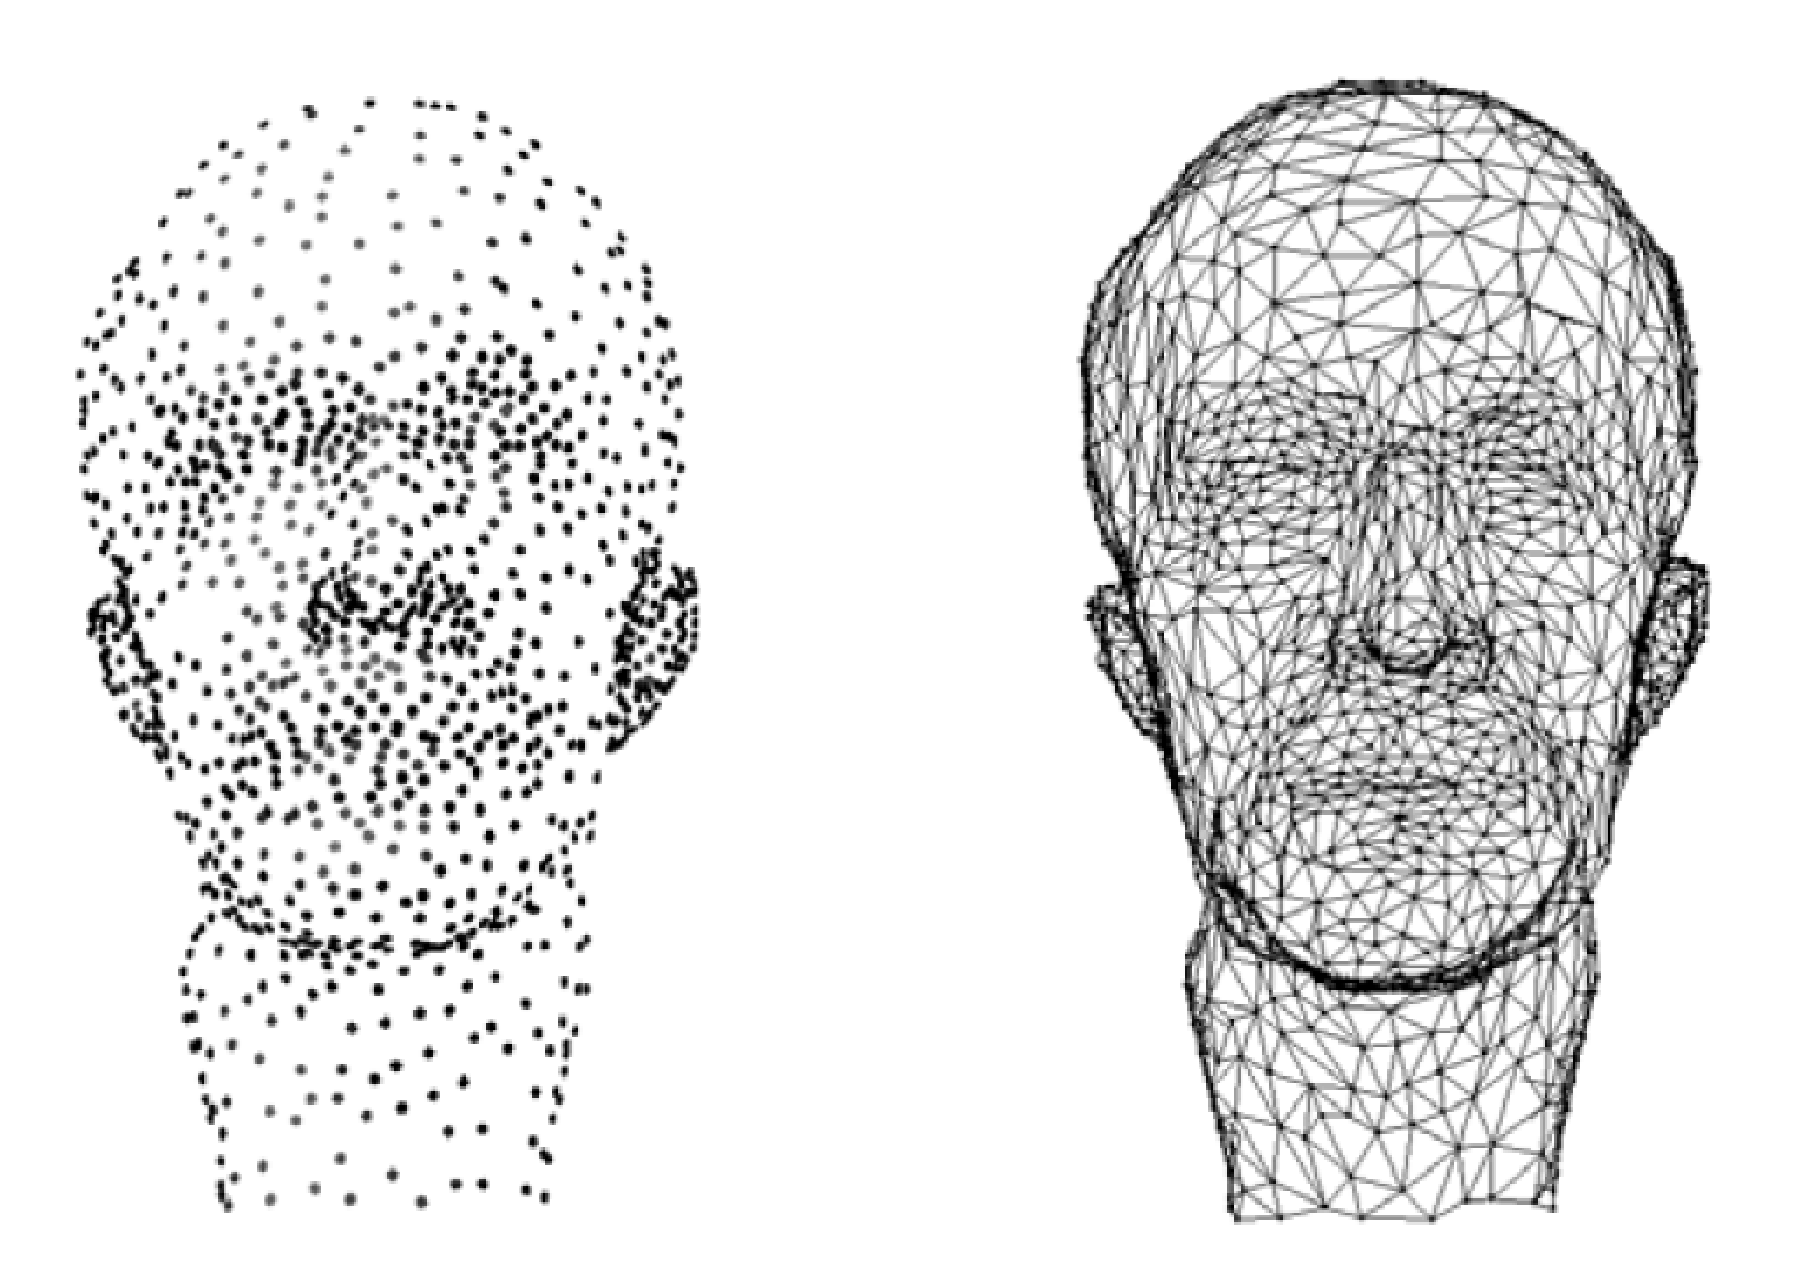
\includegraphics[width=1.00\linewidth]{img/cap04/maxPlanckWinParticulasQEM}\\[
0cm](d)
  \end{minipage}
	
\end{tabular}
\caption{M�todos de simplifica��o propostos por~\cite{Pauly2002}. \textbf{(a)}
Clusteriza��o Incremental. \textbf{(b)} Clusteriza��o Hier�rquica. \textbf{(c)} 
Simula��o de Part�culas. \textbf{(d)} Simplifica��o Interativas.}
\label{fig:pauly}
\end{figure}
 

%Moenning e Dodgson \cite{Moenning03} aplicou um m�todo que usa uma abordagem
%progressiva que come�ando com um ponto escolhido randomicamente, acrescentamos
%a cada passo no conjunto de representantes j� selecionados a partir de amostras
%que mais distancie deles. Esse ponto � sabidamente um v�rtices do driagrama de
%Voronoi (geod�sico) do conjunto de pontos j� selecionados. Como a determina��o
%desse diagrama � custosa ele os autores propoe substitui-lo por uma
%aproxima��o usando \textit{Fast-Marching Farthest Point} que � descrito a
%seguir:
%\begin{enumerate}
%\item Em primeiro lugar se imerge a nuvem de pontos em um grade regular.
%\item A dist�ncia dessa grade ao conjunto de pontos � calculada de forma
%iterativa a partir da dist�ncia dos v�rtices vizinhos que est�o mais pr�ximos
%\item da superf�cie $\mathbf{\mathcal S}$ que ele.
%\item C�lulas contendo v�rtices cujos pontos mais pr�ximos em $\mathbf{\mathcal
%S}$ s�o diferentes, cont�m faces do diagrama de Voronoi. Dentro dessas c�lulas
%essas faces s�o aproximados por um pol�gono planar.
%\end{enumerate} 

%Na verdade s� precisamos tratar as c�lulas adjacentes ao v�rtice mais distante
%de $\mathbf{\mathcal S}$.

%aplicou o princ�pio de \textit{Fast-Marching Farthest
%Point}, introduzida por Eldar et al.\cite{Eldar1997} no contexto de amostragem
%em
%imagens. O m�todo ultiliza um abordagem progressiva que come�a com 
 
 
 %que n�o requer nenhuma reconstru��o de superf�cies a priore. O
 %Algoritmo pode gerar uma representa��o em multiresolu��o e
 %progressiva de forma eficiente.

Os algoritmos citados acima criam uma nuvem de pontos simplificada realizando uma amostragem do modelo, ou seja, definindo um subconjunto da nuvem de pontos original ao remover iterativamente pontos de acordo com uma m�trica de erro.
Enquanto estes m�todos s�o simples e eficientes, suas estrat�gias de
simplifica��o n�o garantem uma distribui��o global uniforme. Al�m disso, os
erros proposto por estes m�todos por vezes n�o produzem um boa estimativa, n�o sendo trivial formular m�tricas mais precisas.

Uma maneira sistem�tica de simplifica��o de pontos foi
proposta por Pauly et al.\cite{Pauly2002}, onde v�rios m�todos de simplifica��o
de pol�gonos foram adaptados para pontos. S�o eles:
\begin{itemize}
  \item{\textit{M�todos de Clusteriza��o:} Onde a nuvem de pontos
  $\mathbf{\mathcal P}$ � dividida em subconjuntos. Os pontos deste subconjunto s�o ent�o substitu�dos por um ponto representativo (geralmente seu centroide). Existem dois tipos de clusteriza��o: incremental, onde clusters
 s�o criados sistematicamente crescendo regi�es atrav�s da agrega��o de pontos
vizinhos; e o hier�rquico, onde clusters s�o criados tomando a nuvem de pontos original e dividindo-a em conjuntos menores.}
  \item{\textit{Simplifica��o Iterativa:} Onde repetidamente seleciona-se pares
  de pontos e junta-os em um s�. Note que para cada jun��o, h� um acr�scimo no
  erro total. No entanto, cria-se uma lista ordenada com todos pares poss�veis, colocando no topo a jun��o que provoca o menor erro. Pares de pontos s�o ent�o aglomerados de forma que o erro seja m�nimo. Para avaliar o
  erro de jun��o dos pares de pontos � usada uma adapta��o do \texit{Quadric
  Error Metric}\abbrev{QEM}{\texit{Quadric Error Metric}} apresentado para
  malhas poligonais em~\cite{Garland1997}.}
  \item{\textit{Simula��o de Part�culas:} Onde h� uma distribui��o aleat�ria
  de um n�mero $\mathbf{n}$ de pontos na superf�cie, tal que
  $|\mathbf{\mathcal{P}^}^\prime| = n$. Ent�o cada ponto � considerado copmo uma
part�cula que aplica for�as de repuls�o �s vizinhas, espalhando-se at� que a
  distribui��o desejada seja alcan�ada.}
\end{itemize}
  
Como discutido em \cite{Pauly2002}, o m�todo de clusteriza��o incremental � o
que possui o maior erro m�dio, seguido pelo m�todo hier�rquico, simula��o de
part�culas e do m�todo iterativo, que possui menor erro. A distribui��o dos
pontos produzida pelos m�todos de clusteriza��o se apro'xima da distribui��o
original, que � desej�vel em alguns caso. Entretanto, simula��o de
part�culas � a alternativa mais vi�vel quando se deseja um densidade uniforme ou
um controle da densidade local da distribui��o. M�todos de clusteriza��o s�o os mais
eficientes devido a sua simplicidade. Clusteriza��o incremental, simplifica��o iterativa e simula��o de part�culas requerem uma capacidade grande de mem�ria por ser linear no n�mero de amostras, enquanto a
clusteriza��o hier�rquica depende apenas do tamanho do modelo simplificado. O autor discute que as tr�s t�cnicas operam diretamente na nuvem de pontos, ao inv�s de reconstruir a superf�cie a priori e s� ent�o aplicar a simplifica��o. A Figura~\ref{fig:pauly} ilustra estes m�todos.

\section{Simplifica��o Baseada em \textit{Splats}}

Como discutido no cap�tulo \ref{cap:02}, para preencher buracos entre os pontos
de forma mais eficiente, representa��es baseadas em pontos s�o frequentemente
estendidas para representa��es baseadas em \textit{Splats}~\cite{Zwicker2001},
onde a superf�cie � aproximada por discos ou elipses. Esta representa��o � de
especial interesse no contexto de renderiza��o, onde os \textit{splats}
facilitam a concep��o de algoritmos eficientes~\cite{Ren2002,BotschW2002,Botsch2003,marroquim07} que gerem imagens de alta qualidade.

Embora a representa��o baseada em \textit{splats} seja bastante utilizada na
pr�tica, muitos esquemas de simplifica��o tomam apenas o centro do \textit{splat} em considera��o (como discutido na se��o anterior).
A ideia � primeiro gerar o conjunto de pontos na qual a densidade se adapta a
curvatura da superf�cie e em um processo posterior, converter os pontos
em \textit{splats} pela analise local de sua vizinhan�a, e assim estimando sua
normal e seu tamanho. Em contraste, t�cnicas de simplifica��o
baseadas em \textit{splat}, exploram toda a geometria do disco ou elipse para
obter o conjunto de \textit{splats} que recobrem a superf�cie. No entanto, estas
t�cnicas s�o computacionalmente mais intensas. 

Wu e Kobbelt~\cite{WuK04} desenvolveram uma t�cnica de simplifica��o
otimizada baseada em \textit{splats} que explora a flexibilidade de modelos de
pontos, ou seja, sem informa��o de topologia. Utilizando um esquema de otimiza��o
global � computada uma
aproxima��o de toda a superf�cie com um conjunto m�nimo de \textit{splats} que
satisfaz um erro global pr�-determinado. 


\begin{figure}[ht]
\centering
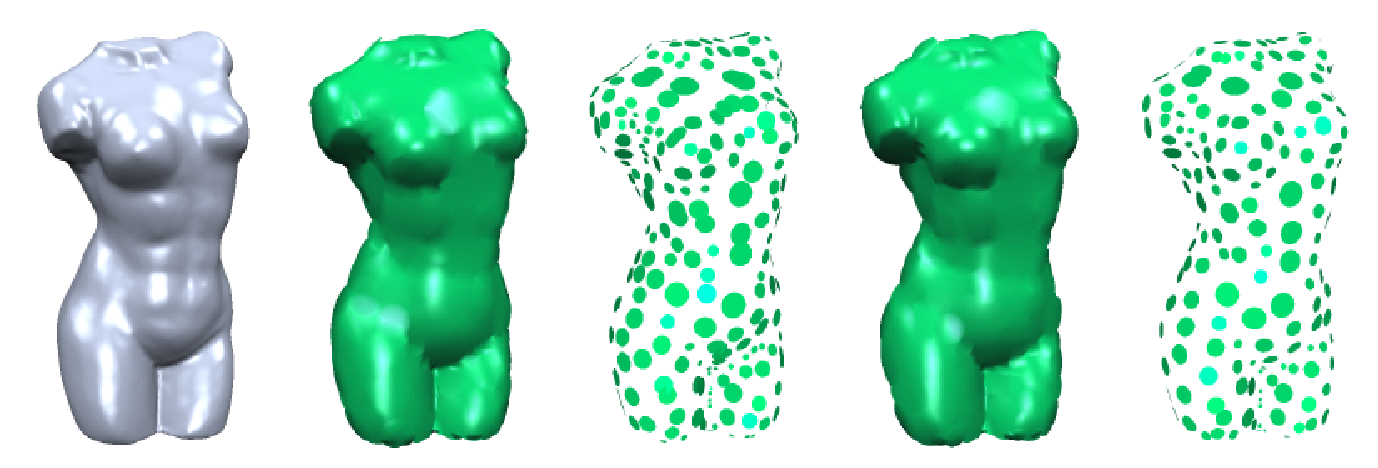
\includegraphics[width=15.0cm]{img/cap04/wu04Iteractive} 
\caption{ \textbf{Esquerda:} Modelo de um torso feminino $171.000$ pontos.
\textbf{Meio:} Modelo aproximado por $422$ \textit{splats} ap�s o segundo passo
(sele��o gulosa). \textbf{Direita:} $333$ \textit{splats} ap�s
finalizado o terceiro passo (otimiza��o global usando sistemas de part�culas)
\textbf{Direita-Meio} e \textbf{Esquerda-Meio} s�o a renderiza��o
dos \textit{splats} usando filtro EWA. Note a melhor distribui��o dos
\textit{splats} ap�s passo de otimiza��o global}
\label{fig:wu04}
\end{figure} 


O objetivo da simplifica��o otimizada � computar um conjunto m�nimo de
\textit{splats} $\mathbf{\mathcal{T}=\{\mathbf{s}_j}\}$ que aproxime o conjunto
original $\mathbf{\mathcal{P}}$ com um erro abaixo de uma toler�ncia
$\mathbf{\varepsilon}$. Para inicializar o algoritmo, em uma fase de pr�-processamento, para cada ponto ${\mathbf{p}_i}$ propriedades locais da superf�cie como vetor normal $\mathbf{n}_i$ e 
densidade $\mathbf{\omega}_i$ s�o calculadas baseados em uma vizinha�a local. Dependendo da
aplica��o, pode-se decidir entre \textit{splats} circulares ou el�pticos. Um
\textit{splat} circular e definido por um centro ${\mathbf{c}_i}$, normal
${\mathbf{n}_i}$ e um raio ${\mathbf{r}_i}$; no caso el�ptico o raio
${\mathbf{r}_i}$ � substitu�do por dois vetores ${\mathbf{t}_i^1}$ e
${\mathbf{t}_i^2}$ que definem os eixos principais da elipse.
Para assegurar o erro $\mathbf{\varepsilon}$ m�ximo, uma nova m�trica de dist�ncia
\textit{splat}-ponto � introduzida: para um ponto
${\mathbf{p}_i}$ a dist�ncia ao \textit{splat} ${\mathbf{\mathcal T}}$ �
definida como sendo a proje��o ortogonal no plano do \textit{splat} ${\mathbf{s}_j}$:
\begin{equation}
 dist(\mathbf{p}_i,\mathbf{\mathcal T}) = dist(\mathbf{p}_i,\mathbf{s}_j) =
 |\mathbf{n}_i^{\mathit T}(\mathbf{p}_i - \mathbf{c}_i)|
\label{eq1}
\end{equation}
\noindent se
\begin{equation}
 || (\mathbf{p}_i - \mathbf{c}_i) - \mathbf{n}_j^{\mathit T}(\mathbf{p}_i -
 \mathbf{c}_i) - \mathbf{n}_j ||^2 \leq \mathbf r_j ^2
\label{eq:circular}
\end{equation}
no caso de um \textit{splat} circular ou
\begin{equation}
 (  \mathbf{t}_j^{1^{\mathit T}}(\mathbf{p}_i - \mathbf{c}_i) )^2  + 
 (\mathbf{t}_j^{2^{\mathit T}}(\mathbf{p}_i - \mathbf{c}_i))^2 \leq 1
\label{eq:eliptico}
\end{equation}
se for um \textit{splat} el�ptico. Se $\mathbf{p}_i$ projetar no interior de v�rios
\textit{splats}, a dist�ncia m�nima � escolhida. Se nenhum $\mathbf{s}_j$ for encontrado pelas equa��es \ref{eq:circular} ou \ref{eq:eliptico}, sua dist�ncia � definida como $dist(\mathbf{p}_i,\mathbf{\mathcal T}) = \infty$.
 
A simplifica��o otimizada segue tr�s passos. No primeiro passo � computado o
\textit{splat} m�ximo para cada ponto ${\mathbf{p}_i}$ cujo erro � limitado por
um $\mathbf{\varepsilon}$. Come�ando por uma semente $\mathbf{p}_i$, 
o \textit{splat} $\mathbf{s}_i$ crescem adicionando os vizinhos
de acordo com sua distancias calculada usando \ref{eq:circular} para
\textit{spalt} circular ou \ref{eq:eliptico} para el�ptico. Este �ltimo
adapta-se melhor a curvatura da superf�cie. Em um segundo passo, para o conjunto
inicial de \textit{splats}, um subconjunto
que cobre a superf�cie sem que haja buracos entre os vizinhos � selecionado
usando um procedimento guloso.
 
Por �ltimo, o procedimento guloso anterior � otimizado usando um procedimento
global. A ideia e iterativamente substituir subconjuntos de \textit{splats}
por um novo subconjunto que tenha mesmo elementos ou um que tenha um melhor
distribui��o, j� que o procedimento anterior � baseado em decis�es locais e
geralmente redundante ou possuindo um distribui��o desigual. A ideia � usar um
sistemas de part�culas como em~\cite{Pauly2002,Tuk}, diferenciando na forma
como as part�culas interagem. A figura~\ref{fig:wu04} mostra o
efeito desta simplifica��o otimiza��o quando o �ltimo passo � finalizado.

Wu el al.~\cite{ProgressiveSplat2005} desenvolveram um algoritmo iterativo com
um abordagem gulosa para criar uma representa��o progressiva de \textit{splats}.
Funciona de forma semelhante ao \textit{Progressive Meshes} de
Hoppe~\cite{Hoppe1996}. Especificamente, data um conjunto de pontos s�o criado
\textit{splats} para cada deles. Em seguida, todas as poss�veis opera��es de
\textit{jun��o de} \texti{splats} s�o organizada em um lista de prioridades de
acordo com uma \textit{m�trica de
erro} que avalia o erro causado pela respectiva opera��o de jun��o com o
elemento com menor erro estando no topo.

\begin{figure}[ht]
\centering
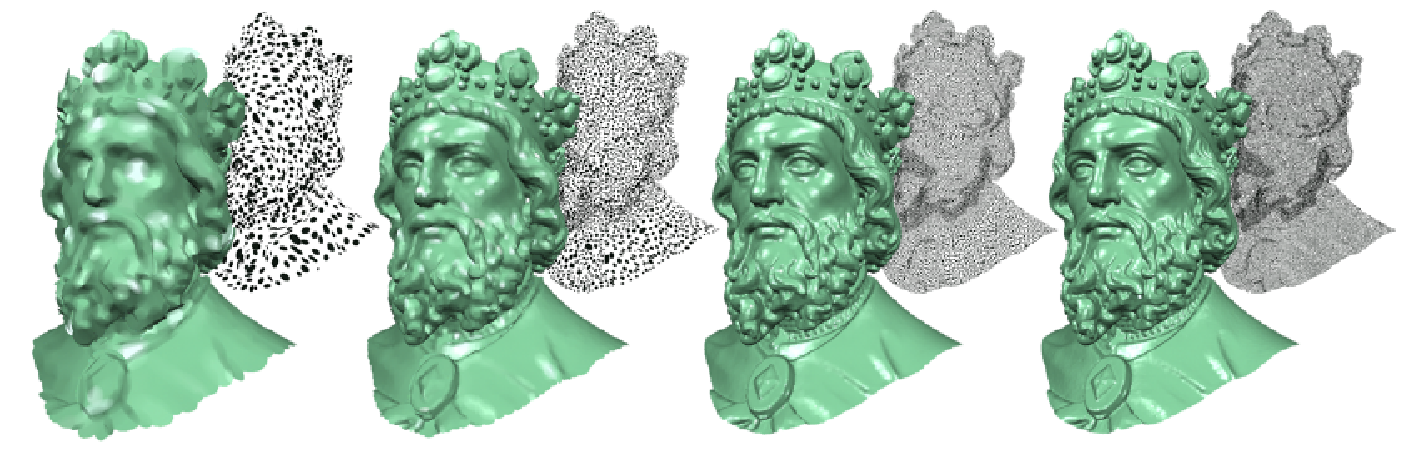
\includegraphics[width=15.0cm]{img/cap04/progressiveSplat} 
\caption{ Representa��o progressiva do modelo de Carlos Magno ($600.000$
 de pontos). Da esquerda para direita, modelos com: $20.00$,
$10.000$, $70.000$ e $600.000$ \textit{splats}}
\label{fig:progressiveSplat}
\end{figure} 

A entrada do algoritmo � um conjunto de pontos $\mathbf{\mathcal P}
= \{\mathbf{1}\ldots\mathbf{p}_i\}$ que s�o transformado em um conjunto
\textit{splats} $\mathbf{\mathcal T  = \{\mathbf{1} \ldots \mathbf{s}_i}\}$ onde
cada \textit{splat} representa um elipse em $3D$ com centro $\mathbf{c}_i$,
normal
$\mathbf{n}_i$ e dois vetores ortogonais $\mathbf{t}_i^1$ e $\mathbf{t}_i^2$

Similar a~ \cite{Pauly2002} e \cite{WuK04} os $k$-vizinhos de $\mathbf{p}_i$, 
$\mathbf{\mathcal{N}}_k(\mathbf{p}_i)$,   
s�o computados de ante m�o, tanto para analisar a superf�cie local 
(computar normal $\mathbf{n}_i$) como para gerar o splat inicial $\mathbf{s}_i$.
Para tanto, um plano $\mathbf{\mathcal{H}}$ � formado para $\mathbf{p}_i$ e
$\mathbf{\mathcal{N}}_k(\mathbf{p}_i)$ definindo $\mathbf{s}_i$ com normal 
$\mathbf{n}_i$ e centro $\mathbf{c}_i = \mathbf{p}_i$. Como os
\textit{splats} iniciais s�o c�rculos, $\mathbf{t}_i^1$ e $\mathbf{t}_i^2$
ser�o dois vetores ortogonais  paralelos a $\mathbf{\mathcal{H}}$ com mesmo
tamanho $\mathbf{r}_i$,

\begin{equation}
 \mathbf{r}_i  = \max_j || (\mathbf{p}_j - \mathbf{c}_i) - \mathbf{n}_i^{\mathit
 T}(\mathbf{p}_j - \mathbf{c}_i) - \mathbf{n}_i || ,
\label{eq:circular}
\end{equation}

\noindent para todo  $\mathbf{p}_j$ $\in$
$\mathbf{\mathcal{N}}_k(\mathbf{p}_i)$. Assim como feito por
\cite{Pauly2002}, $\mathbf{\mathcal{N}}_k(\mathbf{p}_i)$ ser� usado para criar
uma topologia din�mica para auxiliar o processo de jun��o de \textit{splats}.
Sendo assim, � criado um grafo
$\mathbf{\mathcal{G}}(\mathbf{\mathcal{P}},\mathit{E})$ onde uma aresta $(i,j)$ 
pertence a $\mathit{E}$ se $\mathbf{p}_j \in
\mathbf{\mathcal{N}}_k(\mathbf{p}_i)$.
Ent�o um opera��o de jun��o de \textit{splat} $\Phi$ juntar� dois
\textit{splats} $\mathbf{s}_a$ e $\mathbf{s}_b$ associados a dois pontos
$\mathbf{p}_a$ e $\mathbf{p}_b$ de um aresta $\mathbf{e} \in \mathit{E}$
em um \textit{splat} $\mathbf{s}_m$. Assim,  a lista de prioridades conter�
todos as
poss�veis opera��es de jun��o de todas as arestas pertencentes � $\mathit{E}$.  
Para avaliar a opera��o de jun��o dois \texit{splats}, dois erros foram
entendidos. Um que mede o erro pela dist�ncia ($\mathbf{\mathit{L}}^2$) e
outro pelo desvio da normal ($\mathbf{\mathit{L}}^{2,1}$).

\subsubsection{M�trica $\mathbf{\mathit{L}}^2$}

A m�trica $\mathbf{\mathit{L}}^2$ � baseada na dist�ncia Euclidiana. Para
computar o erro causado pela opera��o de jun��o de \textit{splats} $\Phi$
respectivo ao conjunto de pontos originais, uma lista adicional de �ndices
$\{f_i\}$ dos pontos originais � mantida para cada \textit{splat} $\mathbf{s}_i$
onde um �ndice ${i}$ refere a um ponto $\mathbf{p}_i$. 

\begin{figure}[ht]
\centering
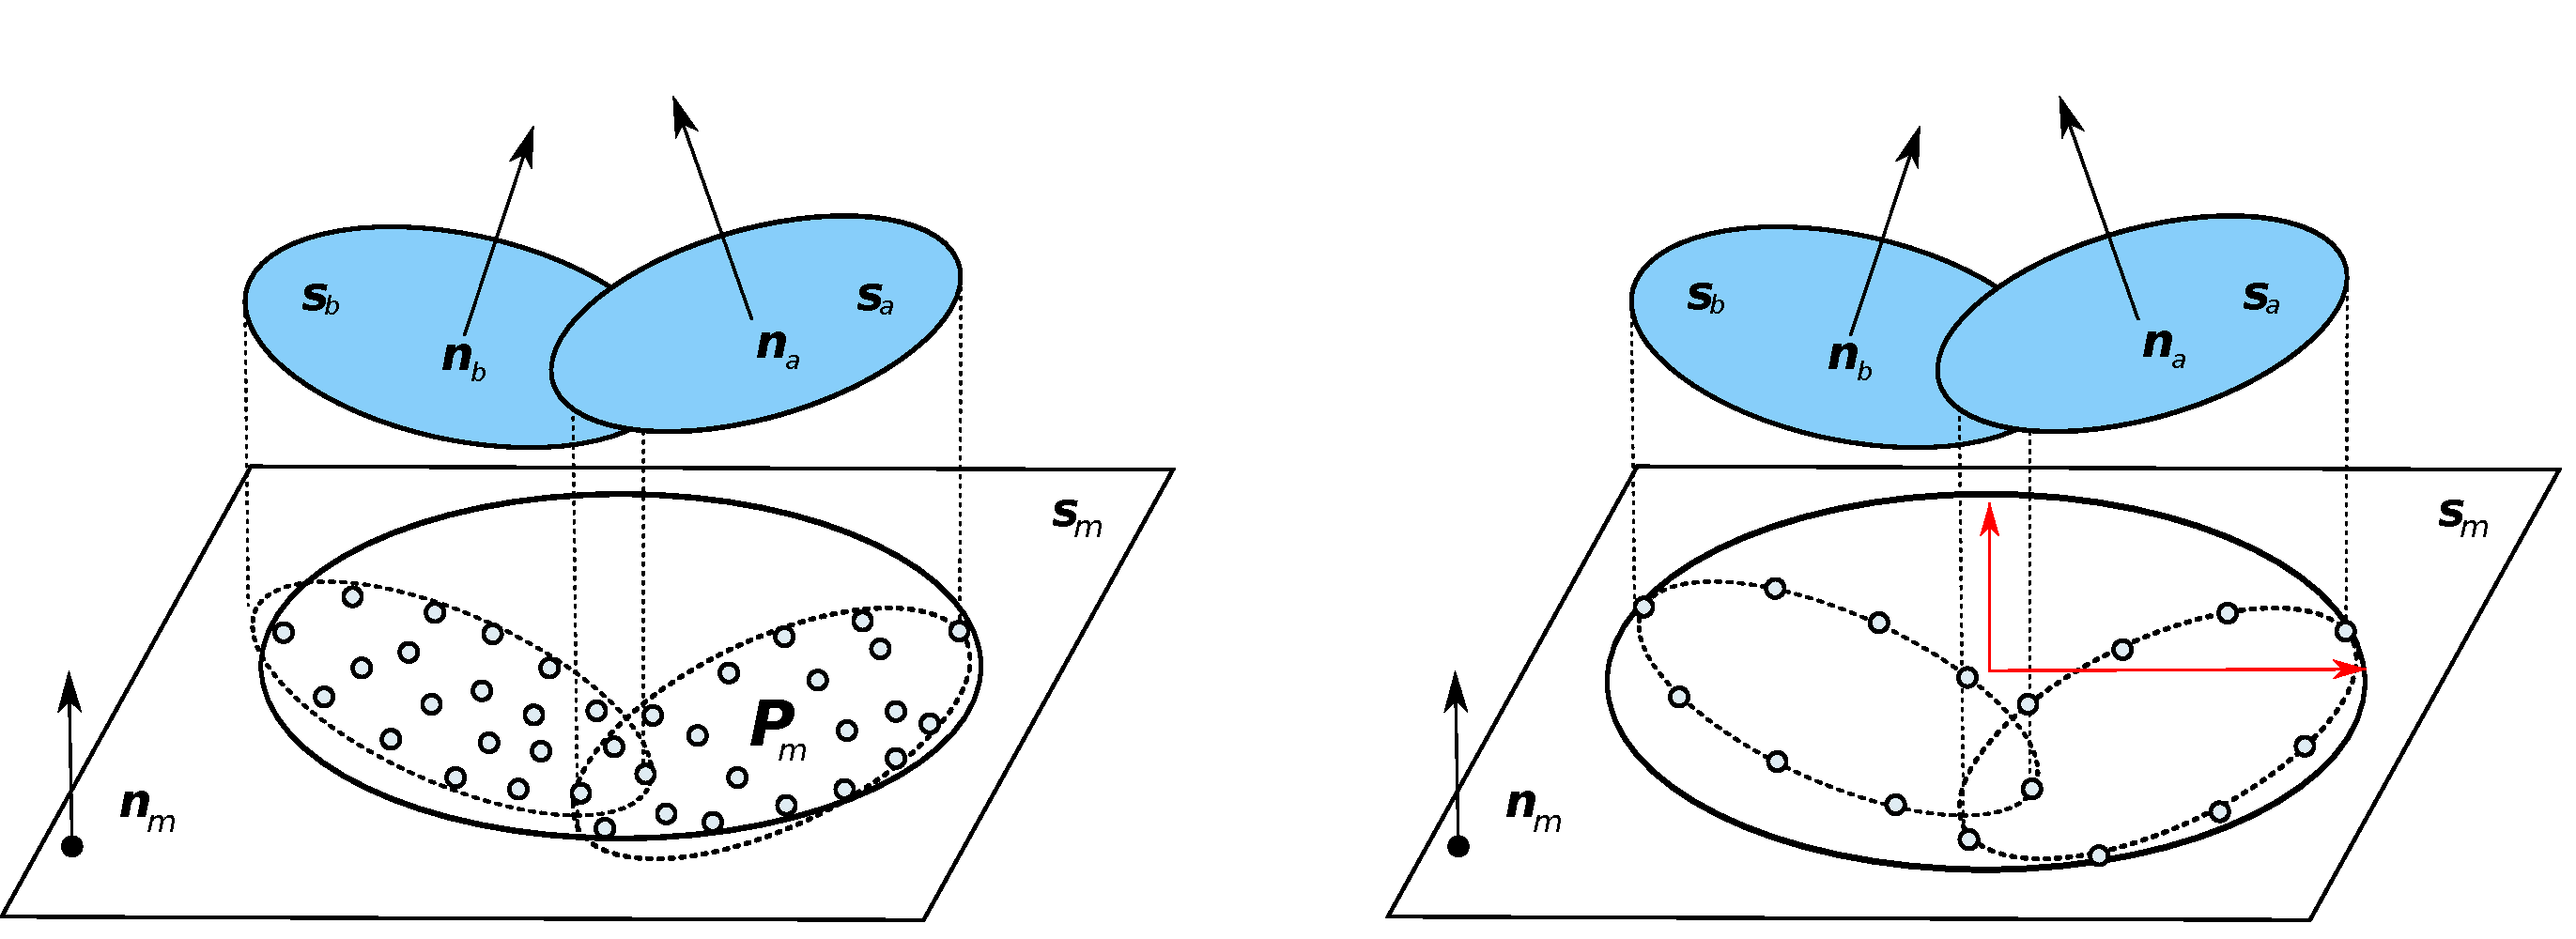
\includegraphics[width=15.0cm]{img/cap04/PosterProgressiveThese} 
\caption{Jun��o dos \textit{splats} de acordo com a m�trica
$\mathbf{\mathit{L}}^2$ (esquerda) e $\mathbf{\mathit{L}}^{2,1}$ (direita) }
\label{fig:merge}
\end{figure}  

Ent�o o erro da jun��o
de dois \textit{splats} $\mathbf{s}_a$ e $\mathbf{s}_b$ em um novo
\textit{splats} $\mathbf{s}_m$ � definido como:
\begin{equation}
 \mathbf{\varepsilon}_{\Phi}  =  ||e||\cdot\mathbf{\sum}_{f \in \{f_m\}}
 |dist(\mathbf{p}_f,\mathbf{s}_m)|^2 ,  \{f_m\} = {f_a} + {f_b}. 
\label{eq:l2}
\end{equation}
Note que o erro � ponderado pela tamanho da aresta, afim de penalizar a jun��o
de \textit{splats} muito distantes
 
Dado a m�trica de erro~\ref{eq:l2} e dois \textit{splats}
$\mathbf{s}_a$ e $\mathbf{s}_b$ para a jun��o, $\mathbf{s}_m$ � determinado
aplicando-se \textit{PCA} no conjunto de pontos $\mathbf{\mathcal{P}}_m =
\{\mathbf{p}_f\}$ diretamente
em $3D$. Assim , teremos o ponto m�dio $\bar{\mathbf{p}}$ e tr�s autovalores
$\lambda_1 \geq \lambda_2 \geq \lambda_3$ e seus autovetores correspondentes
$\mathbf{v}_1$, $\mathbf{v}_2$, $\mathbf{v}_3$.

Assim, $\mathbf{s}_m$ ser�
determinado com centro $\mathbf{c}_m = \bar{\mathbf{p}}$, normal $\mathbf{n}_m
= \mathbf{v}_3$ e os dois eixos $\mathbf{t}_m^1$ e $\mathbf{t}_m^2$ com
dire��es de ter�o as $\mathbf{v}_1$ e $\mathbf{v}_2$ com tamanho respectivo h�
$\sqrt{\lambda_1/\lambda_2}$. Ent�o os tamanho dos eixos ser�o ajustados de
forma que a \textit{splat} englobe todo os pontos $\mathbf{\mathcal{P}}_m$
quando projetados em $2D$ no plano definido por  $\mathbf{s}_m$~\ref{fig:merge}.
 

\subsubsection{M�trica $\mathbf{\mathit{L}}^{2,1}$}
A m�trica de erro $\mathbf{\mathit{L}}^{2,1}$ mede o desvio na dire��o da
normal e foi entendida da m�trica original proposta em~\cite{Cohen2004}. Neste
caso o computo � simples e n�o h� necessidade da lista de �ndices. Dada a
opera��o de jun��o $\Phi$ e dois \textit{splats} $\mathbf{s}_a$ e
$\mathbf{s}_b$, com suas respectivas �reas $|\mathbf{s}_a|$ e
$|\mathbf{s}_b|$, similar a~\ref{eq:l2}, o erro ponderado pelo tamanho da
aresta � definido como:
\begin{equation}
 \mathbf{\varepsilon}_{\Phi}  =  ||e||\cdot|\mathbf{s}_a| +
 |\mathbf{s}_b|\cdot|| \mathbf{n}_a - \mathbf{n}_b ||^2.
\label{eq:l21}
\end{equation}

De acordo com a m�trica  $\mathbf{\mathit{L}}^{2,1}$ o centro do novo
\textit{splat} $\mathbf{s}_m$ � definido como:
\begin{equation}
 \mathbf{c}_{m}  =  \frac{|\mathbf{s}_a|\cdot\mathbf{c}_{a}  +
 |\mathbf{s}_b|\cdot\mathbf{c}_{b}}{|\mathbf{s}_a|+|\mathbf{s}_b|} 
\label{eq:l21c}
\end{equation}
e normal
\begin{equation}
 \mathbf{n}_{m}  =  \frac{|\mathbf{s}_a|\cdot\mathbf{n}_{a} +  
 |\mathbf{s}_b|\cdot\mathbf{n}_{b}}{|\mathbf{s}_a|+|\mathbf{s}_b|} 
\label{eq:l21n}
\end{equation}

Os vetores $\mathbf{t}_m^1$ e $\mathbf{t}_m^2$ s�o calculados da mesma forma
que $\mathbf{\mathit{L}}^{2}$, s� que ao inv�s de projetos o conjunto de pontos
$\mathbf{\mathcal{P}}_m$(que n�o � mais mantido), $n$ pontos ($8$ � o
suficiente) s�o calculados na borda dos \textit{splats} $|\mathbf{s}_a|$ e
$|\mathbf{s}_b|$ e projetados no
plano definido por $|\mathbf{s}_m|$. S� ent�o aplica-se \textit{PCA} e
computa-se os tamanhos de $\mathbf{t}_m^1$ e $\mathbf{t}_m^2$.

Com as duas m�tricas de erro a sequ�ncia de opera��es de jun��o de
\textit{splats} ${\Phi_i}$ e sua opera��o inversa, opera��o de divis�o do
\textit{splat}, podem ser criadas durante o processo de simplifica��o. Esse
procedimento � similar ao proposto para malhas poligonais~\cite{Hoppe1996} com a
grande diferen�a de n�o manter informa��o de topologia.

\section{Discuss�o}
  \chapter{Simplifica��o de Superf�cies baseadas em \textit{Splats}}
Neste cap�tulo apresentaremos um algoritmo para simplifica��o de superf�cies
representada por \textit{splats}. Utilizamos uma abordagem incremental, onde clusters
s�o criados sistematicamente ao crescer regi�es atrav�s da agrega��o de
\textit{splats} vizinhos. Este crescimento � guiado por dois erros: o
\textit{erro perpendicular}, que mede a varia��o dos \textit{splats} na dire��o
da normal; e o \textit{erro tangencial}, que nos fornece uma medida de
cobertura. Partiremos da suposi��o de que o modelo j� possui um representa��o
em \textit{splats} e que inicialmente todos s�o \textit{splats} circulares.

\section{Motiva��o}
Como mencionado no cap�tulo~\ref{cap04}, modelos baseados em pontos
s�o complexos devido � grande quantidade de amostras necess�rias para
represent�-lo, tornando opera��es de simplifica��o uma ferramenta necess�ria para
que seja poss�vel alcan�ar taxas interativas de processamento e visualiza��o;
\texit{splats} s�o muitos usados no contexto de renderiza��o quando se deseja qualidade e efici�ncia (se��o~\ref{cap02:sec:splat}).
Embora a representa��o de superf�cies baseadas em \textit{splats} seja comum na
pr�tica, muitos algoritmos de simplifica��o usa apenas o centro em
considera��o;
a ideia � em um primeiro momento gerar uma superf�cie com uma densidade de
pontos que se ajuste a curvatura da superf�cie e em um processamento posterior,
converter estes pontos em \texit{splats} circulares ou el�pticos. Em
contraste a esta abordagem, simplifica��o de superf�cies baseada em \textit{splats}
levam em considera��o toda a geometria do \textit{splat}.
 
Muitos algoritmos de simplifica��o~\cite{Rusinkiewicz2000,BotschW2002,EfficenteLOD2003} s�o baseados em
estruturas hier�rquicas. Os pontos s�o organizados em uma estrutura de parti��o
espacial (cap�tulo~\ref{cap03}) e os \textit{splats} criados pela
an�lise local da superf�cie. Estas t�cnicas s�o simples e r�pidas, mas como n�o
h� uma estrat�gias de otimiza��o mais elaborada, os resultados geralmente s�o
conservativos e tendem a produzir uma quantidade significativa de \textit{splats} redundantes.
A fim de produzir amostras com maior qualidade, usaremos uma abordagem gulosa
e incremental para renderiza��o eficiente usando \textit{splats}, onde clusters s�o
criados adicionando vizinhos de acordo com m�tricas de erro definidas a diante (se��es~\ref{cap05:sec:perpendicular}
e~\ref{cap05:sec:tangencial}).
 
\section{Clusteriza��o Incremental}
Um cluster $\mathit{C_0}$ � constru�do adicionando-se 
sucessivamente os vizinhos mais pr�ximos de $\mathbf{s}_j$ a partir de uma semente $\mathbf{s}_j \in \mathbf{\mathcal T}$  escolhida randomicamente. Este crescimento
incremental p�ra quando um limitante $\varphi_p$ (para erro perpendicular) e 
$\varphi_t$ (para o erro tangencial) � alcan�ado. O pr�ximo cluster
$\mathit{C_1}$ � ent�o constru�do seguindo o mesmo processo, com uma nova
semente escolhida na vizinhan�a de $\mathit{C_0}$.
Inicialmente, cada vizinho que possui erro perpendicular abaixo de $\varphi_p$ �
utilizado como poss�vel candidato a membro do cluster. Com isso, o novo
centro $\mathbf{c}_m$ e normal $\mathbf{n}_m$ do \textit{splat}
$\mathbf{s}_m$ que representa o cluster s�o atualizados
(ver~\ref{cap05:sec:centroNormal}). Com $\mathbf{c}_m$ e $\mathbf{n}_m$,
podemos atualizar as extens�es do \textit{splat} $\mathbf{s}_m$
(ver~\ref{cap05:sec:eixos}) e, consequentemente, computar o novo erro tangencial
$\mathbf{e}_t$. Caso este erro esteja acima de $\varphi_t$, a
configura��o do �ltimo vizinho adicionado � estabelecida como o cluster final.
O processo continua at� que todos os \textit{splats} de $\mathbf{\mathcal T}$
perte�am a algum cluster $\mathit C_i$.

\subsection{Centro e Normal}
\label{cap05:sec:centroNormal}
Para calcular o novo centro $\mathbf{c}_m$ e normal $\mathbf{n}_m$, utilizamos uma
soma ponderada pela �rea dos \textit{splat} de acordo com a
equa��o~\ref{eq:l21c} e~\ref{eq:l21n} (m�trica $\mathbf{\mathit{L}}^2$). Assim, dado um conjunto
de \textit{splats}, o centro $\mathbf{c}_m$ e a normal $\mathbf{n}_m$ do novo
\textit{splat} podem ser definidos respectivamente como :

\begin{equation}
 \mathbf{c}_{m}  =  \frac{
 \sum_i{|\mathbf{s}_i|\cdot\mathbf{c}_i}}{\sum_i|\mathbf{s}_m|},
\end{equation}
\begin{equation}
 \mathbf{n}_{m}  =  \frac{
 \sum_i{|\mathbf{s}_i|\cdot\mathbf{n}_i}}{\sum_i|\mathbf{s}_m|}.
\end{equation}

\subsection{Eixos da Elipse}
\label{cap05:sec:eixos}
Similar ao m�todo apresentado na Se��o~\ref{cap04:sec:splats:l21}, a fim de obter os eixos da elipse
$\mathbf{s}_m$, projetamos $8$ pontos da borda das elipses $\mathbf{s}_i$ no
plano definido por $\mathbf{c}_m$ e $\mathbf{n}_m$. Aplicamos \textit{PCA} no
conjunto de pontos projetados $C^\prime $ para obter os autovalores $\lambda_1 \geq \lambda_2 \geq \lambda_3$ 
e autovetores unit�rios $v_1,v_2,v_3$. A dire��o dos eixos da elipse 
$\mathbf{s}_m$ � ent�o definida pelos vetores $v_1$ e $v_2$.
Assumindo que a excentricidade da elipse � dada
por $\sqrt{ \frac{\lambda_1}{\lambda_2}}$, pode-se computar as dimens�es dos eixos
principais como:
\begin{equation}
|t_m^1| = \sqrt{\lambda_1} \cdot \bar{\mathbf{e}},
\end{equation}
 \begin{equation}
|t_m^2| = \sqrt{\lambda_2} \cdot \bar{\mathbf{e}},
\end{equation}
onde
\begin{equation}
\bar{\mathbf{e}}  =  \frac{\max_{q \in C^\prime } \{
(\langle q,v_1 \rangle^2)\cdot\lambda_1 + (\langle q,v_2
\rangle^2)\cdot\lambda_2 \} }{\lambda_1\cdot\lambda_2}.
\end{equation}

\section{Erro Perpendicular}
\label{cap05:sec:perpendicular}

\begin{figure}[ht]
\centering
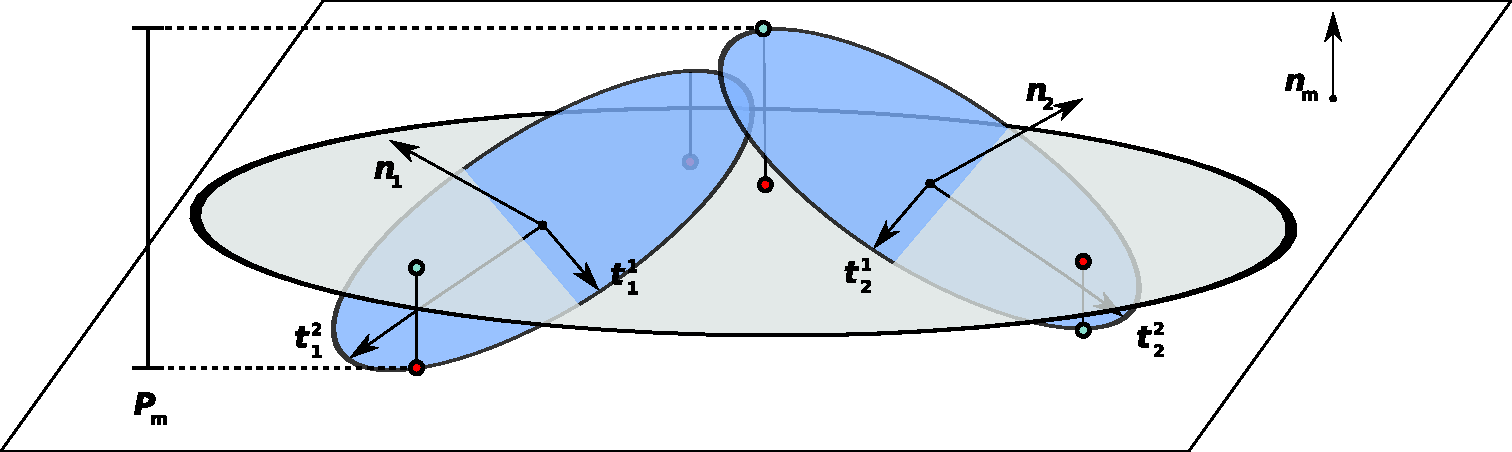
\includegraphics[width=15.0cm]{img/cap05/perpendicular2} 
\caption{O erro perpendicular mede a dist�ncia m�xima dos \textit{splats}
$\mathbf{s}_i$ na dire��o perpendicular ao plano $\mathbf{P}_m$ definido por
pelo \textit{splat} $\mathbf{s}_m$}
\label{fig:merge_splats}
\end{figure}  

O problema de determinar a dist�ncia m�xima de uma elipse
$\mathbf{s}_i$, do conjunto que est� sendo agregado, ao plano da elipse
$\mathbf{s}_m$ (que passa a representar esse conjunto), n�o � t�o imediato como no caso circular. Para
calcular a chamada dist�ncia perpendicular entre $\mathbf{s}_i$ e
$\mathbf{s}_m$, que notaremos como $\mathbf{\mathcal D}(i,m)$, precisamos executar o
seguinte processo. Seja:
\begin{equation}
v(\alpha) = t_{i}^{1} \cos(\alpha) + t_{i}^{2} \sin(\alpha) + c_{i},
\end{equation}
a representa��o param�trica do contorno da elipse $\mathbf{s}_i$ e
${n}_m$ a normal ao plano $P_{m}$ da elipse $\mathbf{s}_m$. Para
maximizar em $\alpha$ a dist�ncia entre $v(\alpha)$ e $P_{m}$ precisamos 
resolver o seguinte problema de otimiza��o:
\begin{equation}
\max_{\alpha \in [0,2\pi]}\langle v(\alpha)-c_{m},{n}_m\rangle = \langle t_{i}^{1},{n}_m \rangle
\cos(\alpha) + \langle t_{i}^{2},{n}_m \rangle \sin(\alpha) + \langle c_{i}-
c_{m},{n}_m \rangle.
\end{equation}
Para  resolver esse problema come�amos igualando a zero a derivada da fun��o
objetiva, o que determina que a solu��o procurada $\alpha_{max}$ deve satisfazer a:
\begin{equation}
\langle t_{i}^{2},{n}_m\rangle \cos(\alpha_{max}) - \langle t_{i}^{1},{n}_m
\rangle \sin(\alpha_{max}) &=& 0  \Longrightarrow \frac{\langle t_{i}^{2},{n}_m
\rangle}{\langle t_{i}^{1},{n}_m \rangle} &=& \tan(\alpha_{max}),
\end{equation}
onde:
\begin{align}
cos(\alpha_{max}) &= \pm \frac{ \langle t_{i}^{1},{n}_m
\rangle}{\sqrt{\langle t_{i}^{1},{n}_m \rangle^{2} + \langle t_{i}^{2},{n}_m
\rangle^{2}}} \\ \nonumber sin(\alpha_{max}) &= \pm
\frac{\langle t_{i}^{2},{n}_m\rangle}{\sqrt{\langle t_{i}^{1},{n}_m\rangle^{2} +
\langle t_{i}^{2},{n}_m\rangle^{2}}} \nonumber.
\end{align}

Para identificar inteiramente $\alpha_{max}$ resta apenas decidir acerca dos
sinais que aparecem nas express�es acima, o que significa distinguir  os casos 
de dist�ncia m�xima e dist�ncia m�nima a $P_{m}$. Isto � feito observando que os 
resultados acima nos permitem escrever $\mathbf{\mathcal D}(i,m)$ da seguinte
forma:
\begin{eqnarray*}
\mathbf{\mathcal D}(i,m) &=& \max_{sign \in \{-1,1\}}{|sign \cdot
\frac{\langle t_{i}^{1},{n}_m\rangle^{2} + \langle
t_{i}^{2},{n}_m\rangle^{2}}{\sqrt{ \langle t_{i}^{1},{n}_m\rangle^{2}
+\langle t_{i}^{2},{n}_m\rangle^{2}}}+\langle c_{i}- c_{m},{n}_m\rangle|} && \\
\mathbf{\mathcal D}(i,m) &=& \sqrt{\langle t_{i}^{1},{n}_m\rangle^{2} +
\langle t_{i}^{2},{n}_m\rangle^{2}}+|\langle c_{i}- c_{m},{n}_m\rangle|.\\
\end{eqnarray*}
Podemos ent�o utilizar $\max_{i}\{\mathbf{\mathcal D}(i,m)\}$ como medida do erro
perpendicular. Alternativamente, podemos estender a defini��o de erro
perpendicular dada na se��o~\ref{sec:SPT} para o caso circular, meramente
substituindo na equa��o~\ref{perpendicular:Circular}, $d_i$ por
$\sqrt{\langle t_{i}^{1},{n}_m\rangle^{2} +\langle
t_{i}^{2},{n}_m\rangle^{2}}$, o que nos permitir� obter:
\begin{eqnarray*}
\mathbf{e}_p  &=&  \max\{\langle c_i-c,n\rangle+ \sqrt{
\langle t_{i}^{1},{n}_m\rangle^{2} +\langle t_{i}^{2},{n}_m\rangle^{2}} \} -\\ 
&& \min\{\langle c_i-c,n\rangle - \sqrt{\langle t_{i}^{1},{n}_m\rangle^{2}
+\langle t_{i}^{2},{n}_m\rangle^{2}}
\}.
\end{eqnarray*}

\section{Erro Tangencial}
\label{cap05:sec:tangencial}
O erro tangencial mede a  diferen�a entre a elipse que representa o cluster
($\mathbf{s}_{m}$) e o conjunto ($\Gamma$) formado pelas proje��es das elipses
que fazem parte do cluster sobre o plano de $\mathbf{s}_{m}$. H� duas maneiras
naturais de avaliar a diferen�a entre dois conjuntos planares. 
A primeira � dada pela �rea da diferen�a sim�trica entre os conjuntos. 
No caso, como $\mathbf{s}_{m}$ contem $\Gamma$, essa diferen�a � simplesmente
$\mathbf{s}_{m}-\Gamma$. A segunda pela maior dist�ncia de um ponto de um
conjunto a outro. Como $\Gamma \subseteq \mathbf{s}_{m}$, podemos nos restringir 
a encontrar o ponto $q$ em $\mathbf{s}_{m}$ mais afastado de $\Gamma$. 
Para obter computacionalmente a �rea de $\mathbf{s}_{m}
-\Gamma$ ($\mathbf{\mathcal A}(\mathbf{s}_{m}-\Gamma$)), pensamos em duas
estrat�gias :

\begin{figure}[ht]
\centering
\begin{tabular}{cc}
\begin{minipage}[b]{0.4\linewidth}
  	\centering
	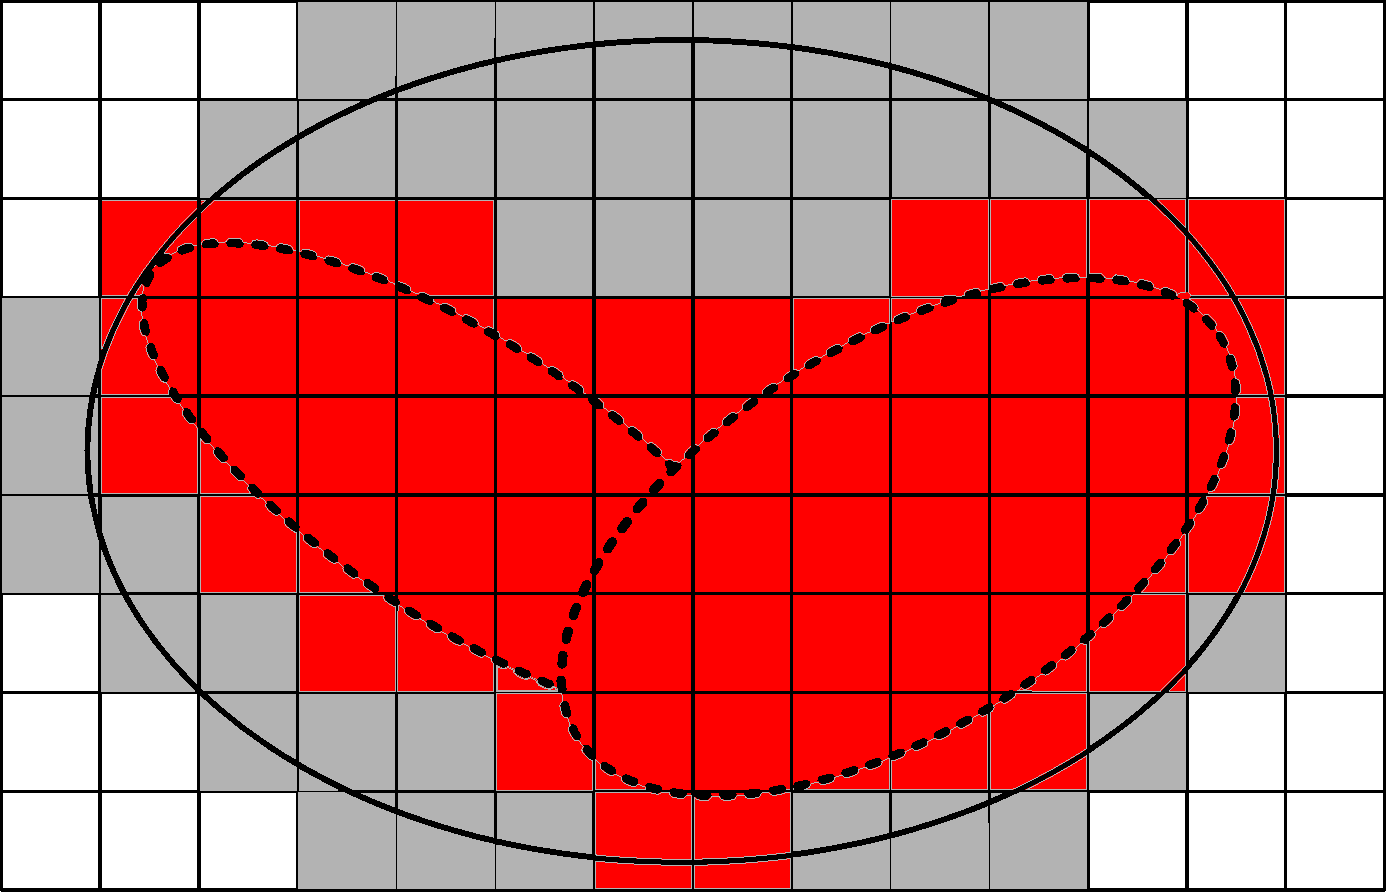
\includegraphics[width=1.00\linewidth]{img/cap05/grade4}\\[0cm](a)
\end{minipage}
\end{tabular}
\caption{}
\label{fig:raia}
\end{figure}
\begin{enumerate}
 \item {A primeira visa obter essa �rea de forma exata. De fato, identificando
 os pontos extremos de cada elipse em rela��o a uma das coordenadas e os ordenando segundo ela, 
 podemos por um algoritmo de varredura de linhas identificar as interse��es dos contornos das 
 elipses de $\Gamma$ e, a partir delas $\mathbf{\mathcal
 A}(\mathbf{s}_{m}-\Gamma$). Esse procedimento, entretanto, tem uma
 complexidade que torna impratic�vel a sua utiliza��o para nossos prop�sitos.
 Para concluir isso, basta considerar que ele � $O(n_{x} \log{n_{x}})$, onde $
 n_{x}$ � o n�mero de interse��es entre elipses de $\Gamma$, o qual j� � quadr�tico
 no n�mero dessas elipses. Al�m disso, o simples c�mputo de uma interse��o entre duas elipses em posi��o gen�rica j� envolve 
 a resolu��o de uma equa��o do quarto grau. Assim, pretender encontrar o valor exato de 
$\mathbf{\mathcal A}(\mathbf{s}_{m}-\Gamma$) � uma tarefa impratic�vel. }

 \item { A segunda forma busca uma solu��o aproximada ao imergir as elipses envolvidas numa malha regular e determinar a
 situa��o de pertin�ncia em rela��o a $\mathbf{s}_{m}$ e $\Gamma$ do centro de cada
 c�lula. Uma c�lula cujo centro pertence a $\mathbf{s}_{m}$ e n�o a $\Gamma$, contribui
 com sua �rea para o c�mputo de $\mathbf{\mathcal A}(\mathbf{s}_{m}-\Gamma$). A
 determina��o da pertin�ncia com rela��o a todas as elipses de $\Gamma$, precisando ser efetuada para um
 n�mero de pontos quadr�tico na resolu��o da malha, prejudica a performance
 dessa alternativa. Isto obriga que se empregue uma malha muito grosseira ou
 que se limite o n�mero de elipses sendo agregadas, tornando, portanto, esta op��o
 tamb�m n�o inteiramente satisfat�ria.}
\end{enumerate}

Tendo em vista as dificuldades apontadas acima na obten��o da �rea de
$\mathbf{s}_{m}-\Gamma$ nos concentramos em obter o erro tangencial via uma
aproxima��o computacionalmente vi�vel da $dist(\mathbf{s}_{m},\Gamma$), a dist�ncia a
$\Gamma$ do ponto de $s_{m}$ mais afastado dele. A determina��o de
$dist(\mathbf{s}_{m},\Gamma$) fica facilitada se assumirmos que o ponto de $\mathbf{s}_{m}$ mais
distante de $\Gamma$ estiver na sua borda. Isso certamente � verdade se o
n�mero de elipses em $\Gamma$ for igual a $2$ e em casos reais, devido a
pr�pria limita��o do tamanho do cluster e do fato do pr�prio processo de
expans�o que gera os clusters n�o fazer curvas acentuadas. Notamos que essa suposi��o n�o
causou distor��es acentuadas no c�lculo do erro tangencial. Se podemos limitar
a busca do ponto mais distante de $\Gamma$ a borda de $\mathbf{s}_{m}$,
podemos aproximar $dist(\mathbf{s}_{m},\Gamma$) de forma aceit�vel e com custo
computacional adequado, da seguinte forma:

\begin{itemize}
\item {O contorno da elipse $\mathbf{s}_m$ que
representa o cluster � discretizado num conjunto, $\mathbf{\mathcal C} =
\{p_1,\ldots,p_8\}$, contendo $8$ de seus pontos. Especificamente,
s�o aqueles que definem com o centro da elipse raias que fazem com o eixo maior um �ngulo m�ltiplo de $45^{o}$.  }
\item {Seja $\mathbf{s}_i$ uma elipse do conjunto $\mathbf{\mathcal T} =
\{\mathbf{s}_1, \ldots,\mathbf{s}_n\}$, que est� sendo condensado, e $\mathbf{s}_i^\prime$ uma
elipse do conjunto $\mathbf{\mathcal T}^\prime = \{\mathbf{s}_i^\prime,
\ldots,\mathbf{s}_n^\prime\}$\ de elipses projetadas sobre o plano definido
por $\mathbf{s}_m$. A dist�ncia de cada um dos pontos ($p_{k} \in $ $\mathbf{\mathcal C}$) em que se discretiza 
$\mathbf{s}_m$ a $\mathbf{s}_i^\prime$  $-$ que notaremos por
$dist(p_{k},\mathbf{s}_i^\prime)$ $-$ � obtida de forma aproximada da forma
indicada abaixo. Os elementos referidos no texto a seguir est�o representados
na Figura~\ref{fig:merge_splats}.}
\end{itemize}
\begin{figure}[ht]
\centering
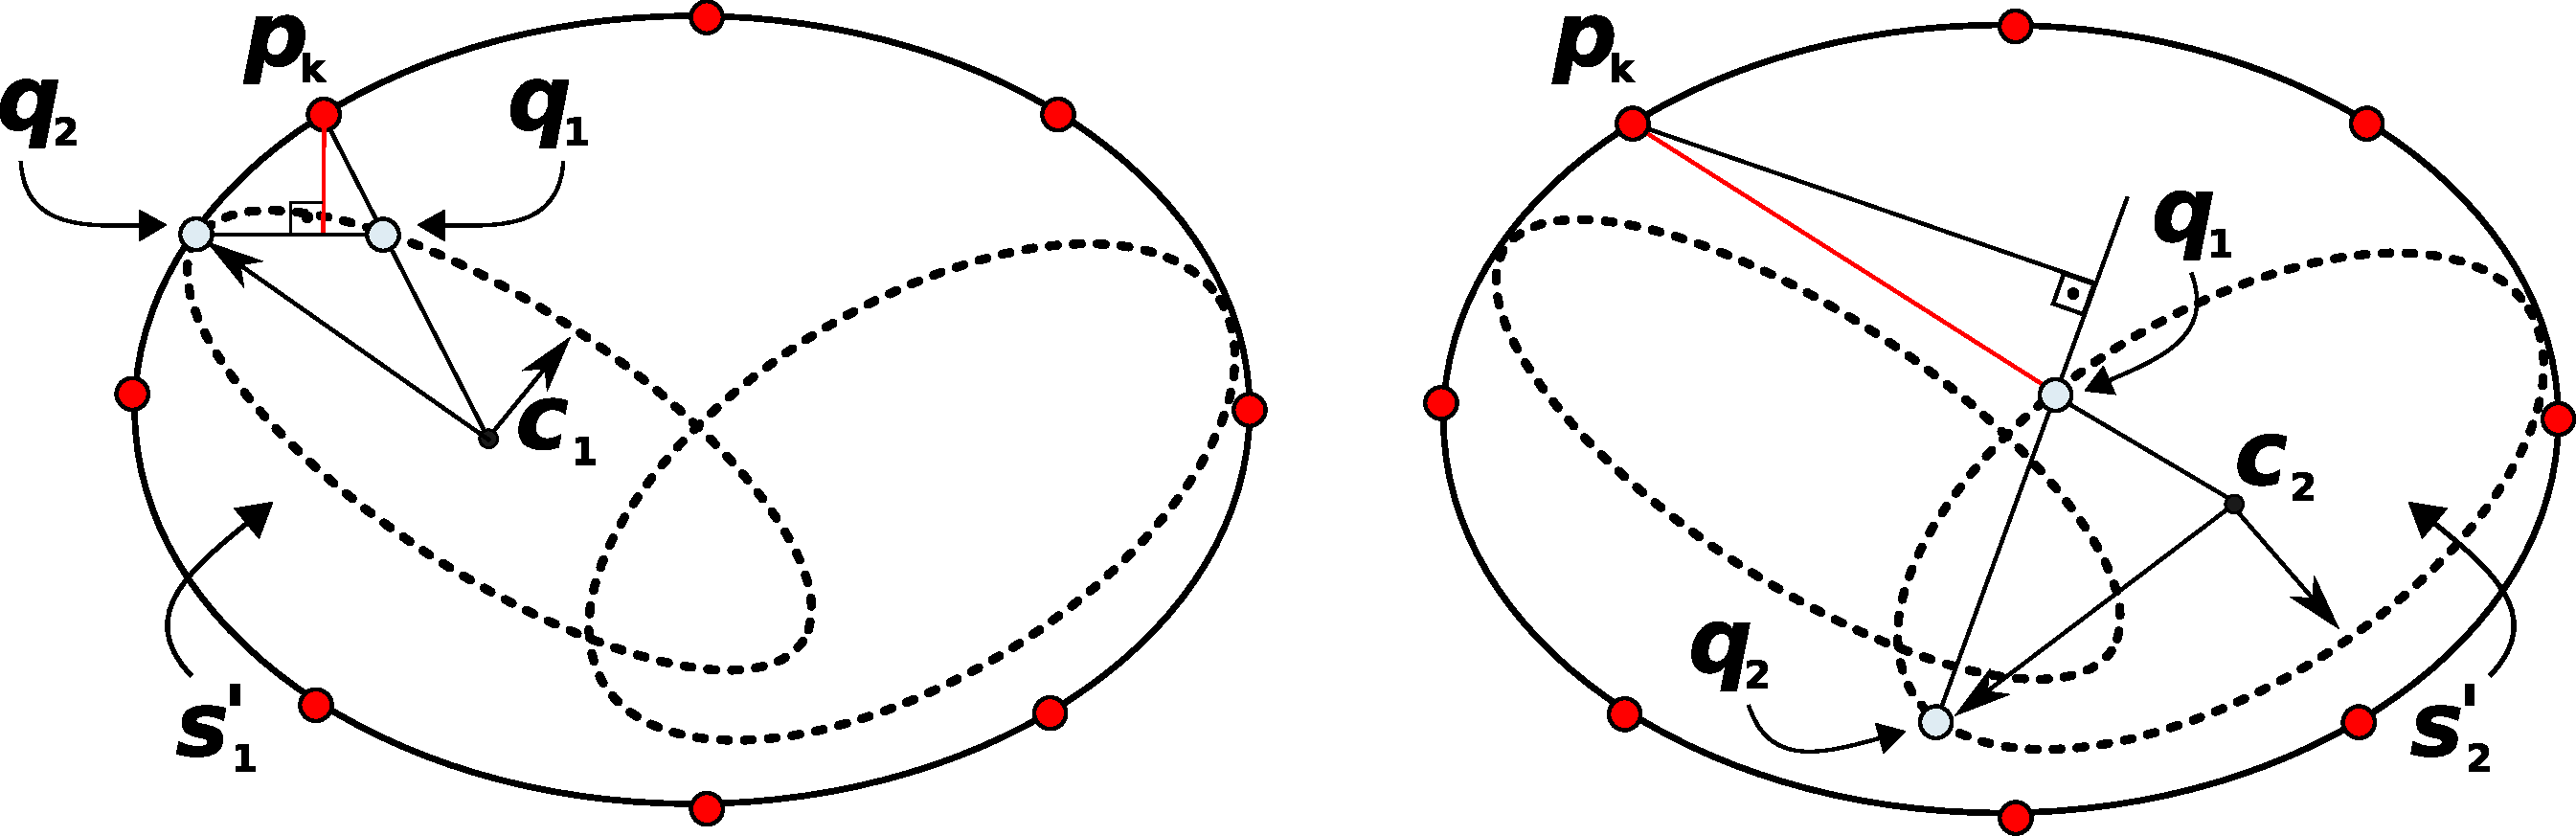
\includegraphics[width=15.0cm]{img/cap05/tangencial}
\centering
\begin{tabular}{cc}
\begin{minipage}[b]{0.4\linewidth}
  	\centering
	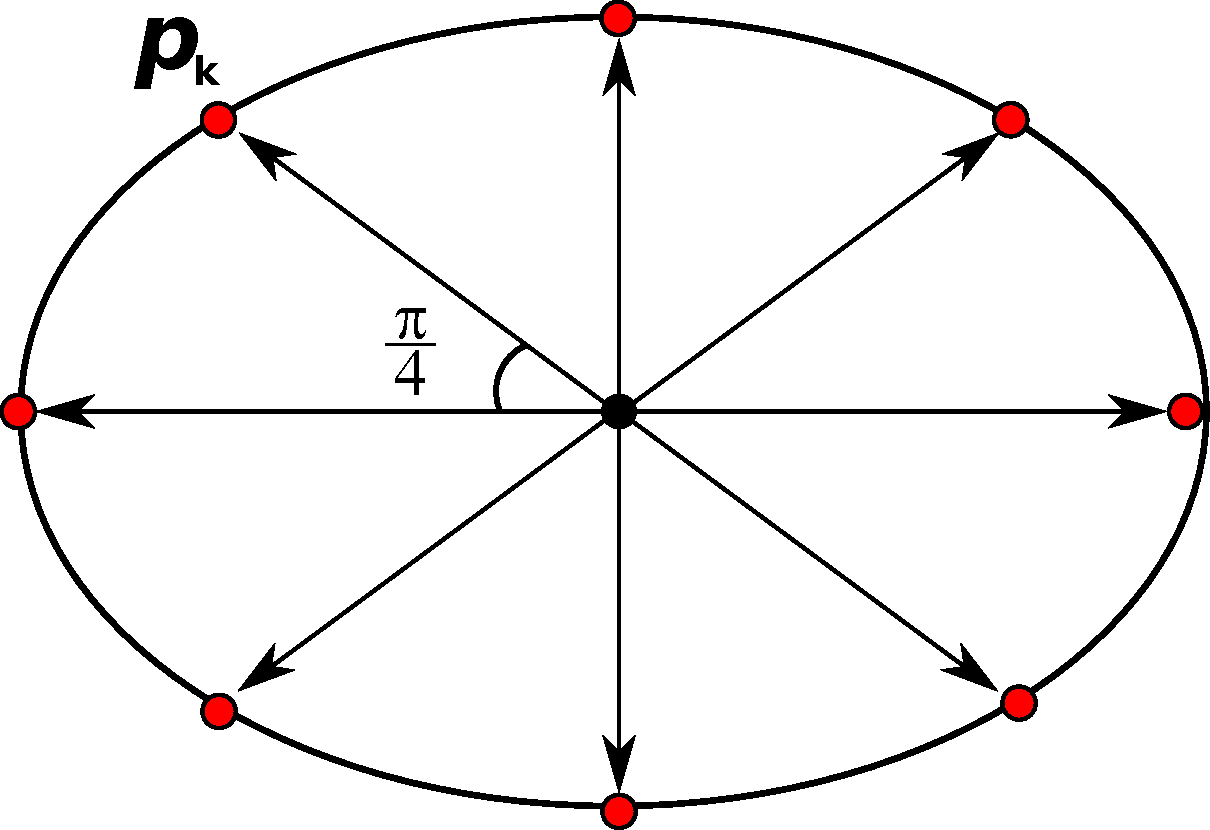
\includegraphics[width=1.00\linewidth]{img/cap05/raias}\\[0cm]
\end{minipage}
\end{tabular}
\caption{}
\label{fig:raia}
\caption{ Dist�ncia aproximada de uma elipse $\mathbf{s}_i^\prime$ do conjunto
das elipses projetadas $\mathbf{\mathcal T}^\prime$ ao contorno de $\mathbf{s}_m$
discretizado em $8$ pontos. O segmento em vermelho representa o erro tangencial.}
\label{fig:merge_splats}
\end{figure}  
\begin{enumerate}
\item {No caso �bvio em que $p_{k} \in  \mathbf{s}_i^\prime$, teremos
$dist(p_{k}, \mathbf{s}_i^\prime) = 0 $.}

\item {Caso contr�rio, considere o segmento de reta delimitado pelo ponto $q_{1}$,  
onde a raia $[ c_{i}, p_{k}]$ corta a elipse  $\mathbf{s}_i^\prime$, e $q_{2}$ sendo a extremidade do eixo 
maior de $\mathbf{s}_i^\prime$  que est� mais pr�xima de $p_{k}$.}

\item {Computa-se a dist�ncia de  $p_{k}$ a $[q_{1}, q_{2}]$ e usa-se essa dist�ncia como 
aproxima��o de $dist(p_{k}, \mathbf{s}_i^\prime))$.}
\end{enumerate}

Utilizando a dist�ncia aproximada definida acima, se obt�m para cada $p_{k}$
sua dist�ncia ao conjunto de elipses $\mathbf{\mathcal T}^\prime$ $-$ dado por
$ \min_{ \mathbf{s}_i^\prime \in  \mathbf{\mathcal T}^\prime}
(dist_{p_k \in \mathbf{\mathcal C}}(p_{k}, \mathbf{s}_i^\prime))$. O erro
tangencial ser� finalmente obtido tomando-se a maior dessas dist�ncias. Ele pode, ent�o, ser expresso por:


\begin{eqnarray}
e_t &=& \displaystyle\max  \{ \min_{ \mathbf{s}_i^\prime \in  \mathbf{\mathcal T}^\prime}
(dist_{p_k \in \mathbf{\mathcal C}}(p_{k}, \mathbf{s}_i^\prime)) \}\\\nonumber 
\end{eqnarray}

\section{Resultados}
A Tabela~\ref{cap05:tabelasimplificacao} exp�e os resultados das simplifica��es de $3$ modelos. O
limitante para erro perpendicular $\varphi_p$ foi tomado como sendo o dobro da
dist�ncia do vizinho mais pr�ximo � semente: $2 \cdot \min_{p \in \mathbf{\mathcal{N}}_k(\mathbf{s}_{seed})}dist(\mathbf{s}_{seed},p)\quad$. 
O limitante tangencial $\varphi_t$ foi
tomado como sendo a dimens�o do eixo menor da semente $||\mathbf{t}_{seed}^1||$.
\begin{table}[ht]
\begin{center}
\begin{tabular}{lcc}
\hline
Modelo  & N� \textit{Splats} Originais &
N� \textit{Splats} Simplifica��o
\\
\hline
\textit{Bunny} 	   & $139990$ & $11258$\\
\hline
\textit{Armadillo} & $172974$ & $11964$\\
\hline
\textit{Dragon}    & $437645$ & $37959$\\
\hline
\end{tabular}
\end{center}
\caption{N�mero de \textit{splats} ap�s simplifica��o usando nosso
algoritmo.}
\label{cap05:tabelasimplificacao}
\end{table}

\begin{figure}[ht]
\centering
\begin{tabular}{cc}
\begin{minipage}[b]{0.4\linewidth}
  	\centering
	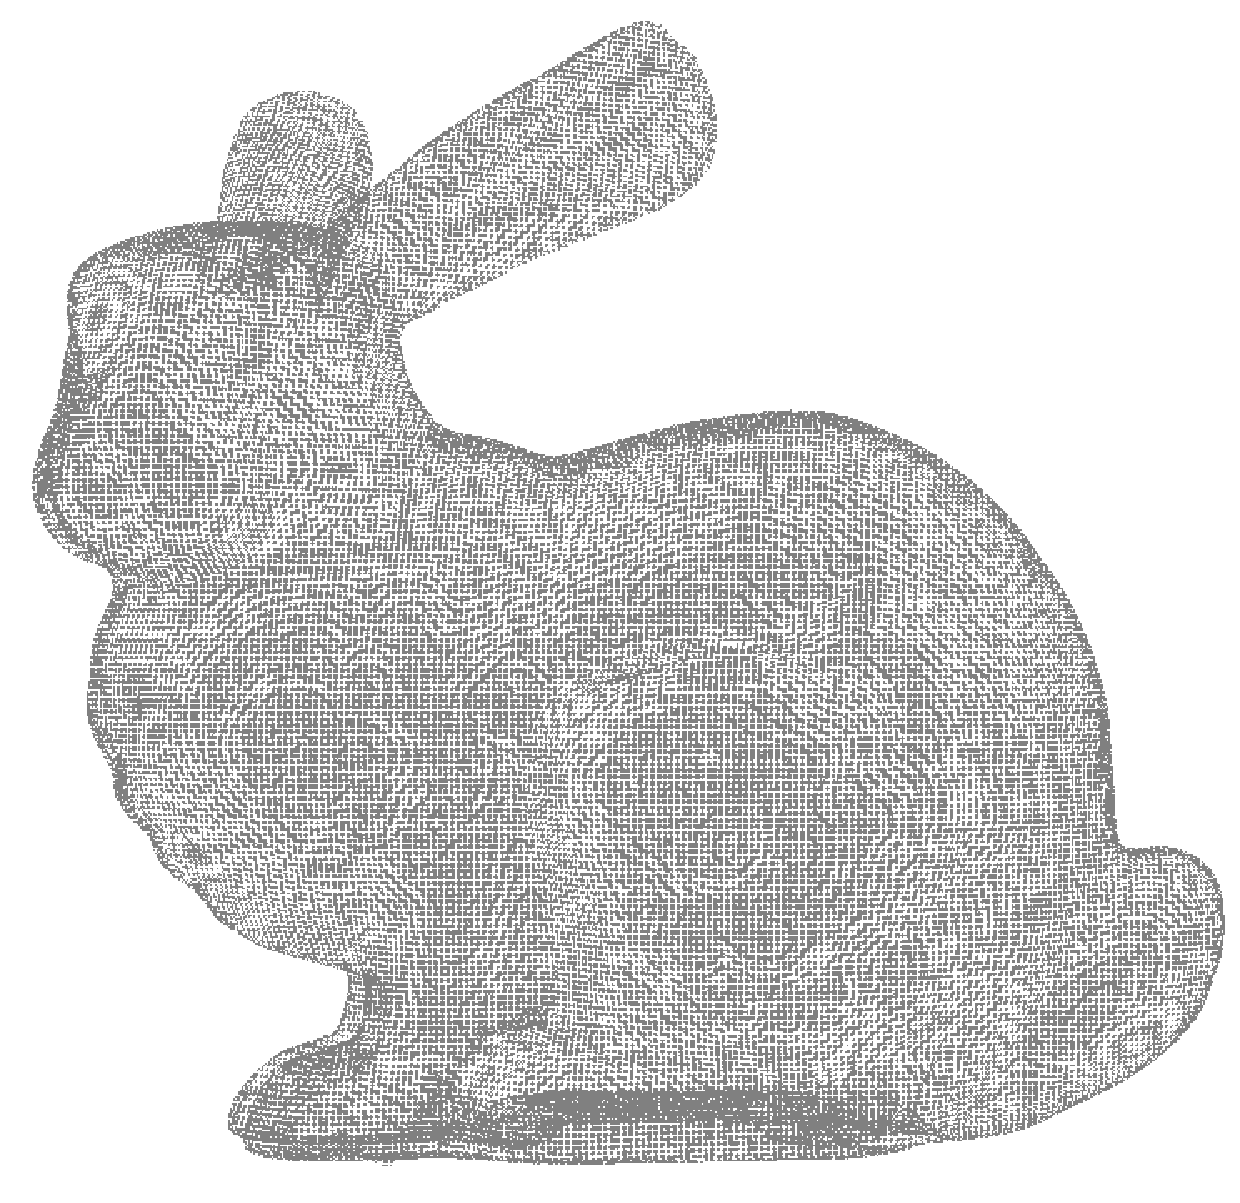
\includegraphics[width=1.00\linewidth]{img/cap05/bunnyTotalpdf}\\[0cm](a)
\end{minipage}
   \hfill
&\begin{minipage}[b]{0.4\linewidth}
   	\centering
	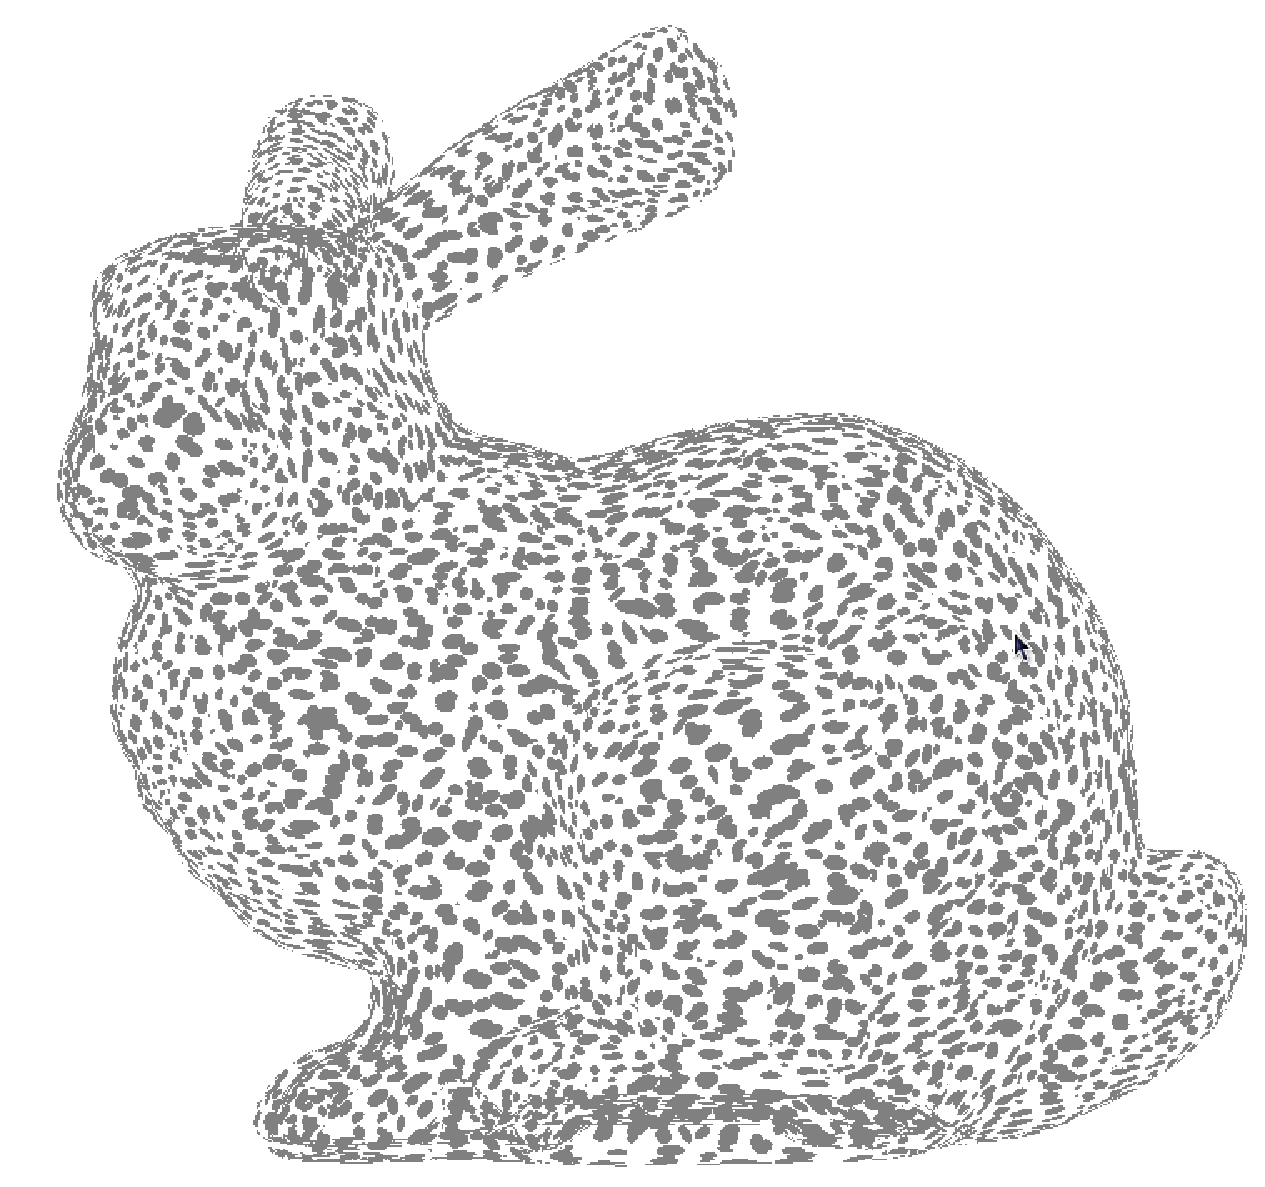
\includegraphics[width=1.00\linewidth]{img/cap05/bunnySpdf}\\[0cm](b)
\end{minipage}
\\
\begin{minipage}[b]{0.4\linewidth}
	\centering
	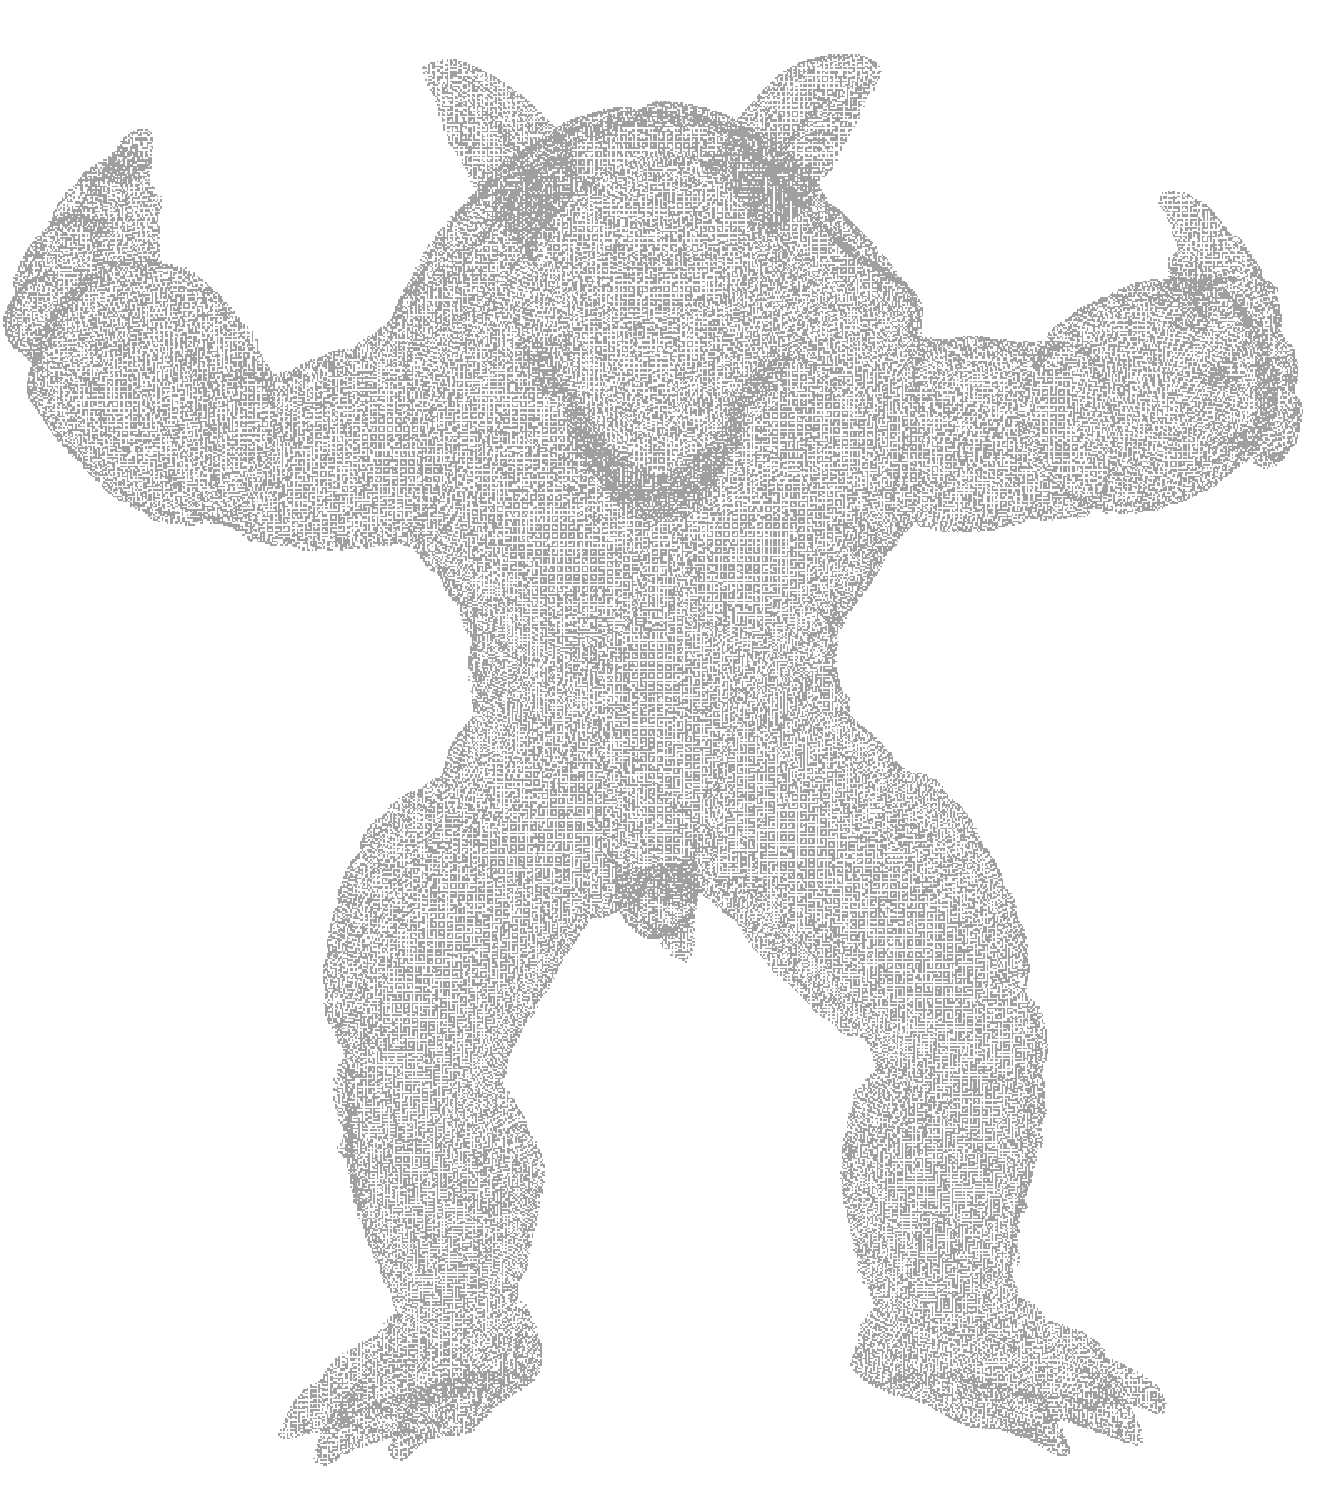
\includegraphics[width=1.00\linewidth]{img/cap05/ArmadilhoTotal}\\[0cm](c)
\end{minipage}  
  \hfill
\centering
&\begin{minipage}[b]{0.4\linewidth}
    \centering
    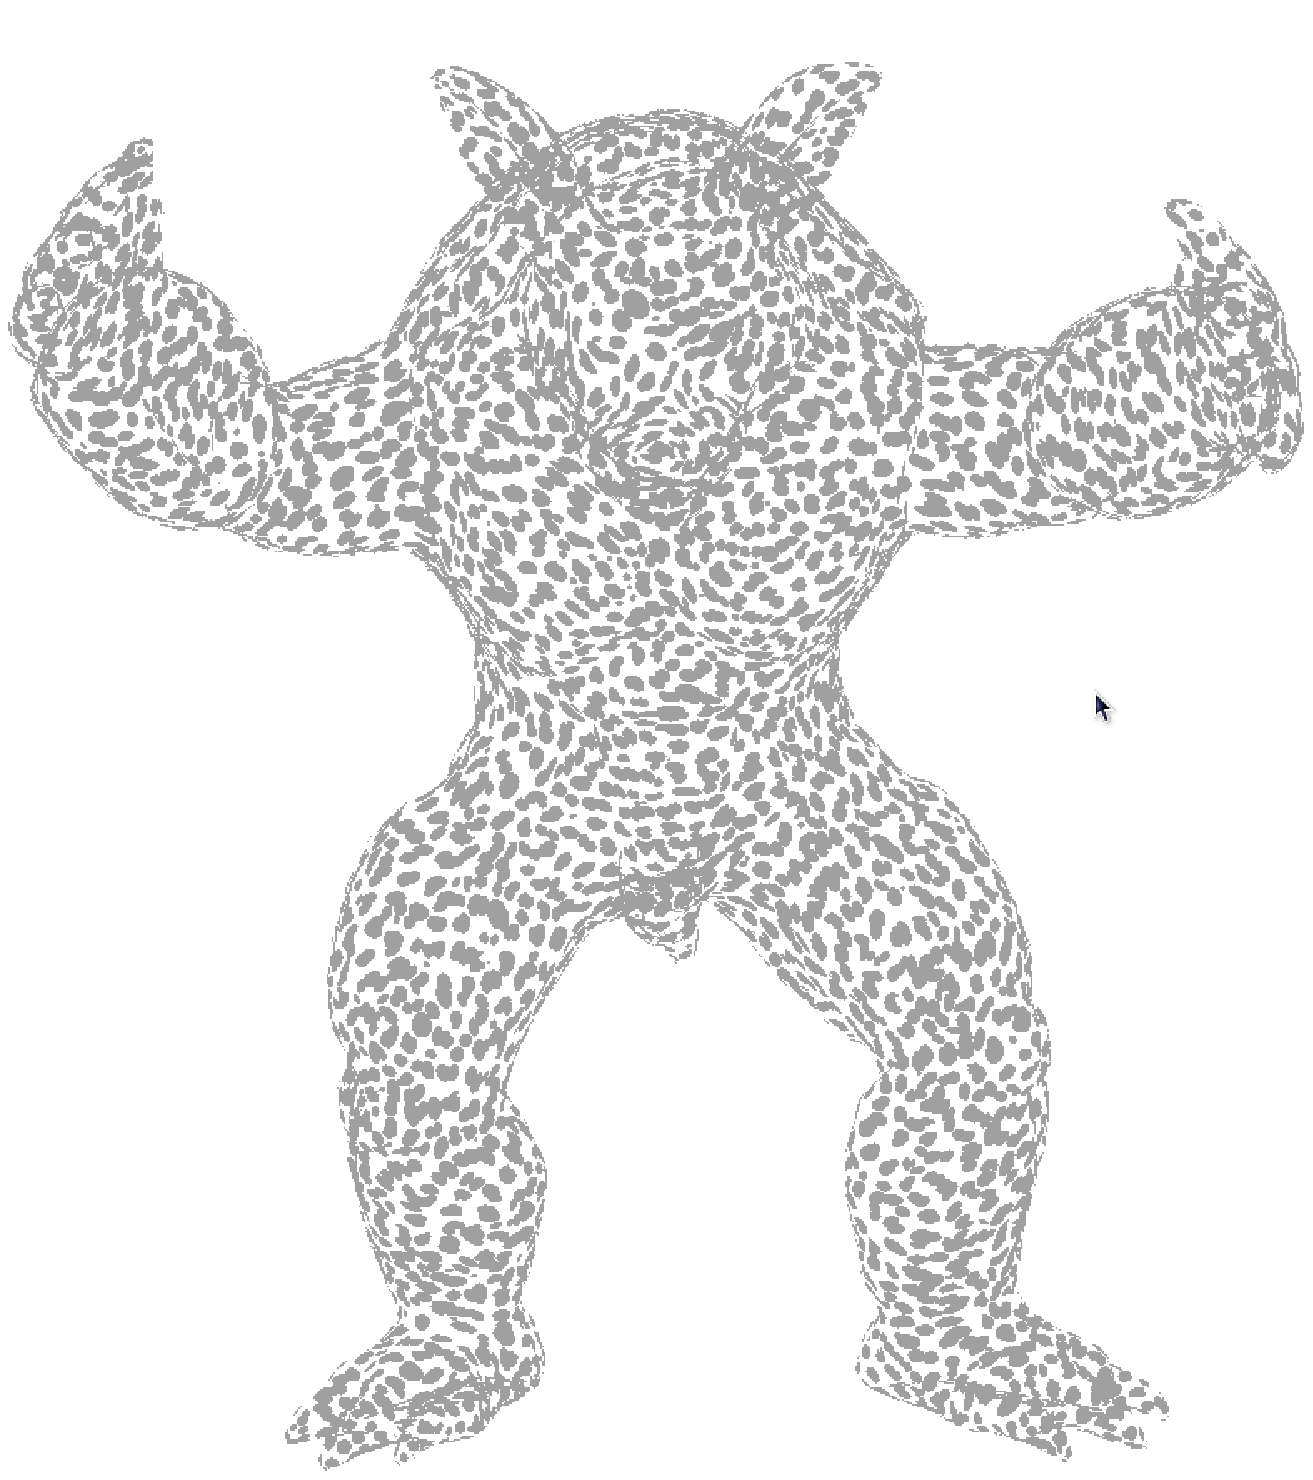
\includegraphics[width=1.00\linewidth]{img/cap05/ArmadilhoS}\\[0cm](d)
\end{minipage}
\\
\begin{minipage}[b]{0.4\linewidth}
	\centering
	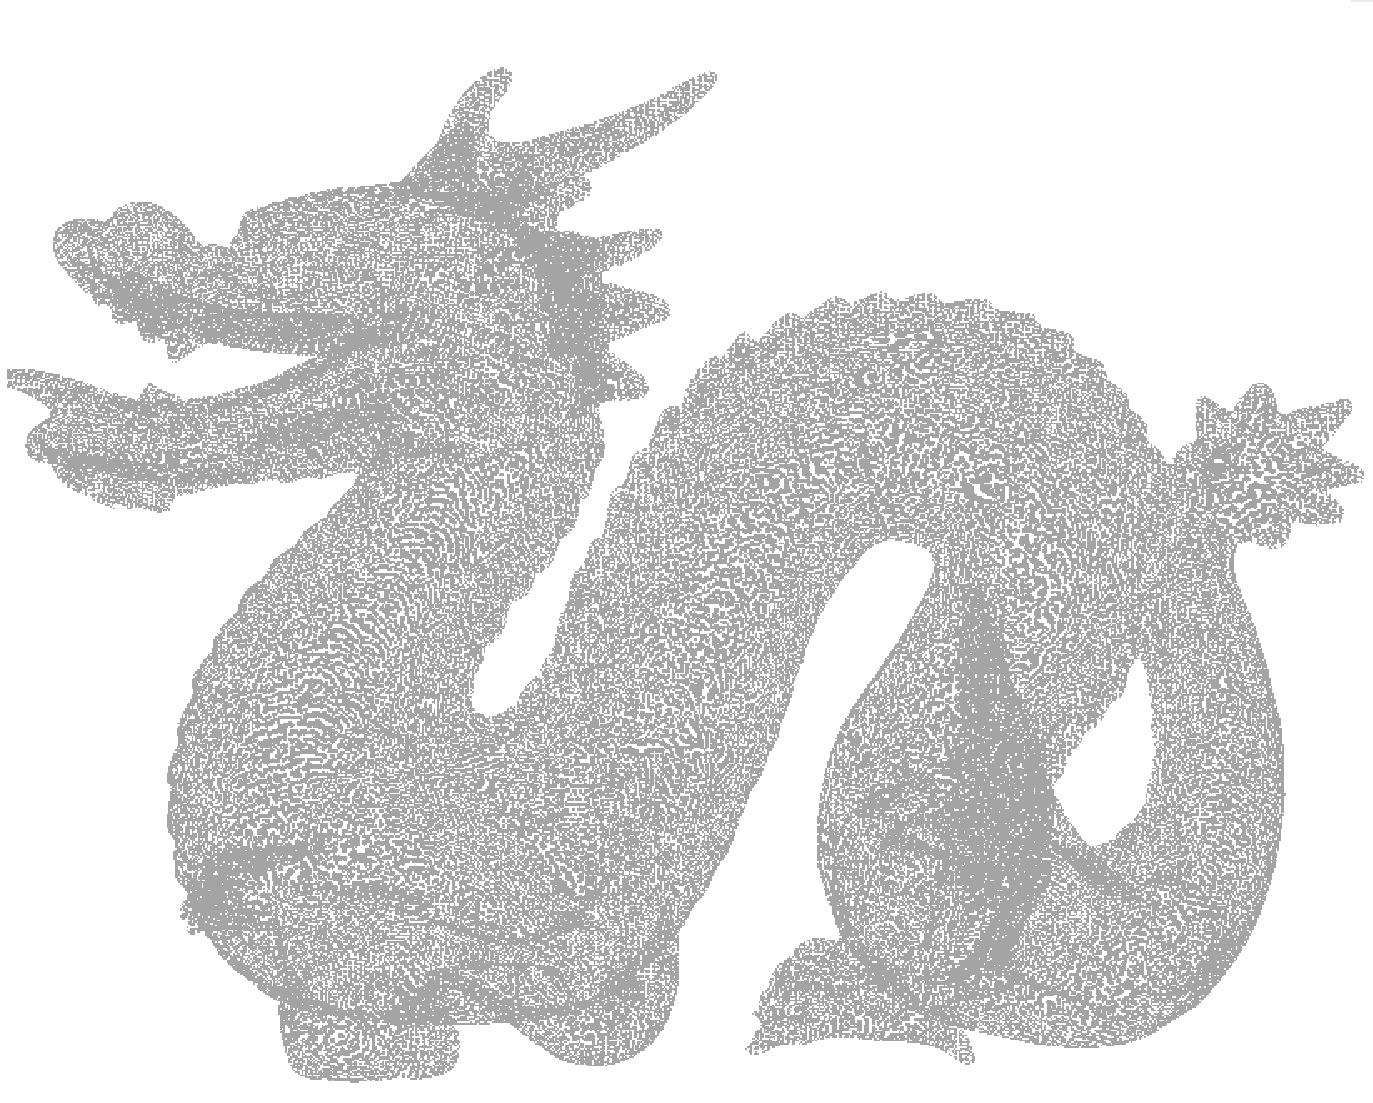
\includegraphics[width=1.00\linewidth]{img/cap05/dragontotal}\\[0cm](e)
\end{minipage}  
  \hfill
\centering
&\begin{minipage}[b]{0.4\linewidth}
    \centering
    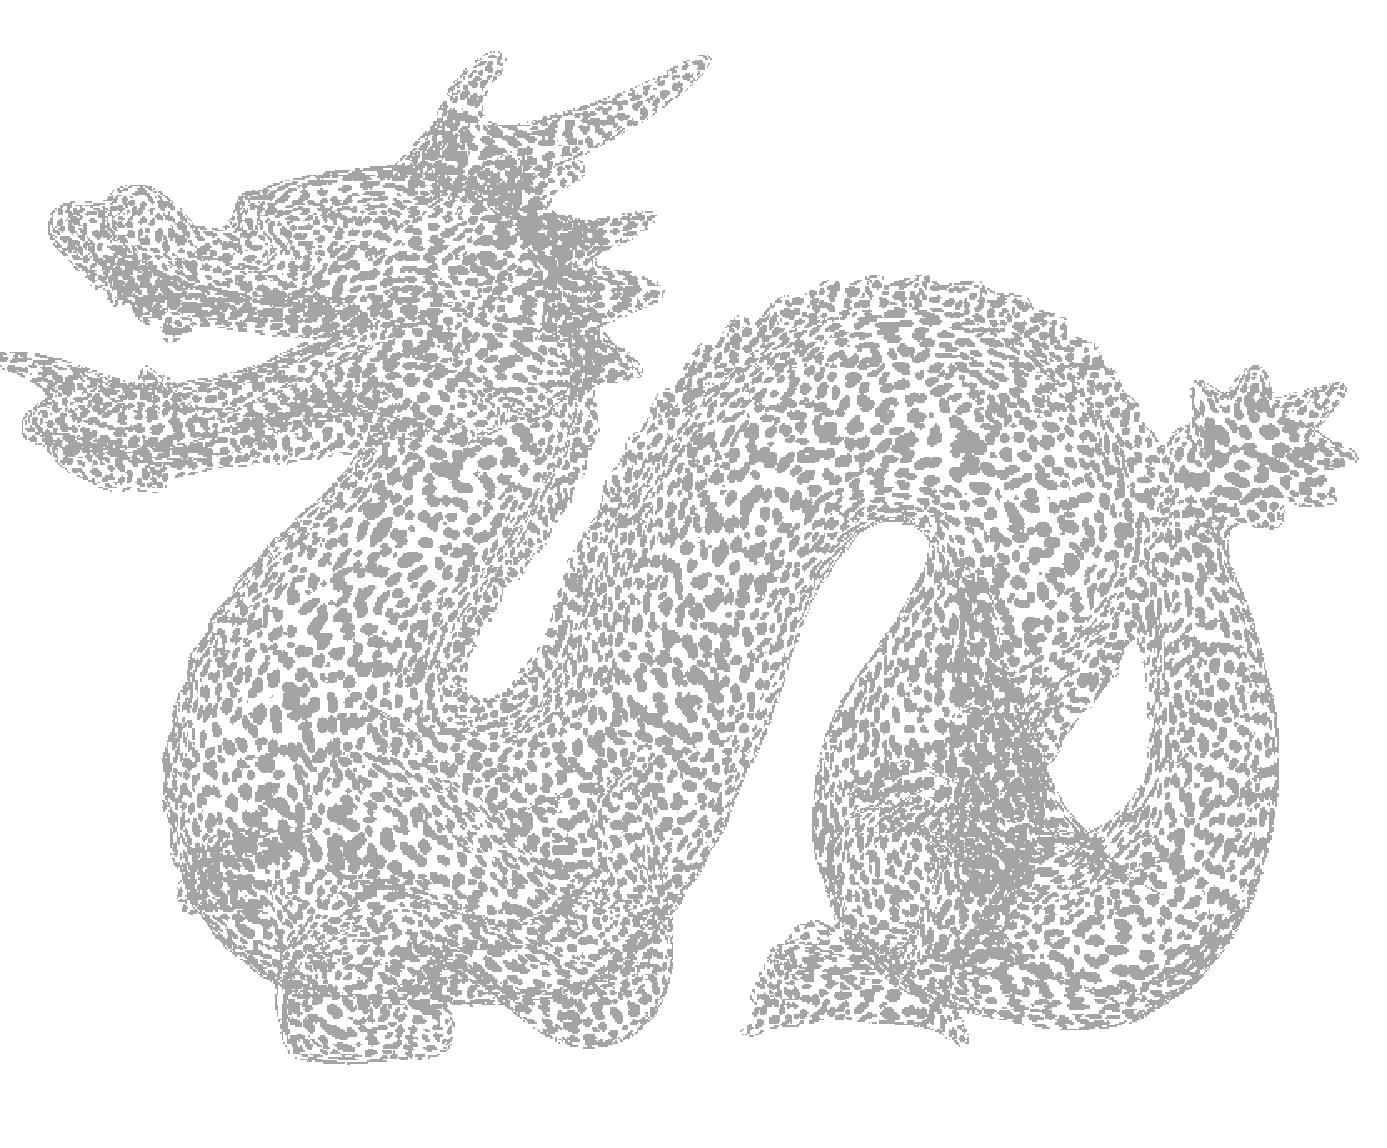
\includegraphics[width=1.00\linewidth]{img/cap05/dragonS}\\[0cm](f)
\end{minipage}
\end{tabular}
\caption{Modelos aprensetados na
tabela~\ref{cap05:tabelasimplificacao}.\textbf{(a)} Modelo \textit{Bunny}
original: $139990$. \textbf{(b)} \textit{Bunny} simplificado: $11258$. \textbf{(c)} Modelo \textit{Armadillo} original: $172974$. \textbf{(d)} Modelo simplificado: $11964$.\textbf{(e)} Modelo \textit{Dragon} original: $437645$
\textbf{(f)} Modelo simplificado $37959$.}
\label{fig:pauly}
\end{figure}

Foi usada uma \textit{K-D Tree} para computar os $k-$vizinhos mais pr�ximos da
semente. Foram usados $32$ vizinhos mais pr�ximos, mas este n�mero � dependendente
da densidade do modelo; sendo assim, o tamanho do cluster fica limitado ao m�ximo de
$32$.

\section{Discuss�o}
Este cap�tulo apresentou um algoritmo de simplifica��o baseado em
\textit{splats} bem como duas extens�es de m�tricas de erro para o caso
el�ptico, o erro perpendicular e o tangencial. O erro perpendicular fornece uma
medida de vari�ncia na dire��o da normal, permitindo distinguir regi�es com
curvatura acentuada de regi�es planares. O erro tangencial nos fornece uma
medida de cobertura, evitando que os cluster cres�am de forma descontrolada e, consequentemente,
cubram �reas desnecess�rias.



  \backmatter
  \nocite{*}
  \bibliographystyle{coppe-unsrt}
  \bibliography{thesis}
  \appendix
  \chapter{C�digo Fonte}

\end{document}
